% =====================================================================
%  Unattended-luggage detection: dataset, detector study, pipeline
%  Two-column, IEEE-like layout built on stock `article` so it compiles
%  anywhere. Swap the preamble for \documentclass{ieeeaccess} on submission.
% =====================================================================
\documentclass[10pt,twocolumn,a4paper]{article}

\usepackage[margin=0.72in,columnsep=0.26in]{geometry}
\usepackage{mathptmx}
\usepackage[T1]{fontenc}
\usepackage[utf8]{inputenc}
\usepackage{amsmath,amssymb}
\usepackage{nicefrac}
\usepackage{graphicx}
\usepackage{booktabs}
\usepackage{multirow}
\usepackage{array}
\usepackage{xcolor}
\usepackage{caption}
\usepackage{titlesec}
\usepackage{enumitem}
\usepackage{microtype}
\usepackage{balance}
\usepackage{cite}
\usepackage{stfloats}
\usepackage[hidelinks]{hyperref}
\usepackage{tikz}
\usetikzlibrary{arrows,positioning,calc,shapes.geometric,fit,backgrounds}

% --- print-safe muted palette for the pipeline figure -------------------
\definecolor{cTeal}{RGB}{ 61,154,139}
\definecolor{cTealBg}{RGB}{228,242,239}
\definecolor{cPurp}{RGB}{106, 79,191}
\definecolor{cPurpBg}{RGB}{234,230,248}
\definecolor{cAmb}{RGB}{191,134, 42}
\definecolor{cAmbBg}{RGB}{250,240,222}
\definecolor{cCor}{RGB}{200, 84, 57}
\definecolor{cCorBg}{RGB}{250,231,225}
\definecolor{cBlu}{RGB}{ 40,105,170}
\definecolor{cBluBg}{RGB}{226,237,247}
\definecolor{cGry}{RGB}{110,115,122}
\definecolor{cGryBg}{RGB}{240,241,243}

\tikzset{
  blk/.style   ={draw=cGry,fill=cGryBg,rounded corners=2.2pt,inner sep=3.4pt,
                 align=center,font=\scriptsize,minimum height=8.2mm},
  teal/.style  ={blk,draw=cTeal,fill=cTealBg},
  purp/.style  ={blk,draw=cPurp,fill=cPurpBg},
  amb/.style   ={blk,draw=cAmb, fill=cAmbBg},
  cor/.style   ={blk,draw=cCor, fill=cCorBg},
  blu/.style   ={blk,draw=cBlu, fill=cBluBg},
  fl/.style    ={->,>=stealth,draw=cGry,line width=0.45pt},
  flb/.style   ={->,>=stealth,draw=cGry,line width=0.45pt,dashed},
  lbl/.style   ={font=\scriptsize\itshape,text=cGry,align=center},
}

% ---------------------------------------------------------------------
% FIGURE SOURCE SWITCH
%   \figpngfalse  -> figures drawn inline as TikZ (vector; use for submission)
%   \figpngtrue   -> figures included from fig1.png / fig2.png
% Regenerate the PNGs with:  make_figs.sh
% ---------------------------------------------------------------------
\newif\iffigpng
\figpngfalse

\captionsetup[table]{font=small,labelfont=bf,skip=4pt}
\captionsetup[figure]{font=small,labelfont=bf,skip=4pt}
\titleformat{\section}{\normalfont\large\bfseries}{\Roman{section}.}{0.6em}{}
\titleformat{\subsection}{\normalfont\normalsize\bfseries}{\Alph{subsection}.}{0.6em}{}
\renewcommand{\thesection}{\Roman{section}}
\renewcommand{\thesubsection}{\Alph{subsection}}
\setlength{\parskip}{0pt}
\setlength{\textfloatsep}{10pt}
\newcommand{\ie}{i.e.,\ }
\newcommand{\eg}{e.g.,\ }

% ---------------------------------------------------------------------
\begin{document}

\twocolumn[
\begin{@twocolumnfalse}
\begin{center}
{\LARGE\bfseries Small-Object Luggage Detection with YOLOv12 and YOLO26:\\[2pt]
A New Annotated Benchmark and Detector-Specific\\[2pt]
Loss and Architecture Improvements\par}
\vspace{10pt}
{\large Constantin Catargiu\par}
\vspace{4pt}
{\small Faculty of Electronics, Telecommunications and Information Technology,\\
Gheorghe Asachi Technical University of Ia\c{s}i, 700506 Ia\c{s}i, Romania\\
\texttt{constantin.catargiu95@gmail.com}\par}
\vspace{14pt}
\end{center}

\begin{abstract}
\noindent\small
Unattended-luggage detection in public spaces is limited less by event logic than
by the detector underneath it: in bird's-eye surveillance imagery almost every
piece of luggage is a small object. Progress on this bottleneck is hard to
measure because the field's benchmarks are small, unannotated, or no longer
distributable. We address this on three fronts. First, we introduce
\textbf{LuggageDataset~v6i}, a fully annotated detection benchmark of
\textbf{12{,}184 images and 57{,}814 luggage instances} across three classes
(backpack, bag, trolley), which provides roughly \textbf{21$\times$ the luggage
annotations} of the largest previously available annotated in-domain set. Second,
we improve both detectors, each along a loss axis and an architectural axis
developed for it: a curriculum area-weighted regression loss and a
level-specialised four-scale head for YOLOv12, and a flattened task-alignment
exponent with a reallocated three-scale head for YOLO26. Against a measured seed
noise floor measured separately for each detector ($0.34$ and $0.25$~mAP,
$\mathrm{df}=8$), \textbf{every reported configuration is trained at three
seeds}. The two axes combined gain \textbf{$+$3.44\%} small-object mAP$_{50}$ on
YOLO26 and \textbf{$+$2.85\%} on YOLOv12 over their baselines, with F1 up
$3.82\%$ and $3.39\%$ --- gains of $9.5$ and $11.0$ standard errors. These come from a controlled study of \textbf{226 training runs} in
which every mechanism is verified live at training time and every
pretrained-weight transfer is measured rather than presumed. Third, we compare
the two detectors directly by applying each one's winning mechanisms to the
other on identical data, and find that \emph{nothing transfers in either
direction}: all four cross-model transfers are nulls on the primary metric, and
both the depth optimum and the ``vestigial coarse level'' finding invert. We
trace each failure to an implementation detail the configuration surface hides
--- the presence of a distributional box loss, the presence of NMS, and whether
a deepened branch propagates or terminates --- and show that the two axes are
additionally \textbf{sub-additive}, delivering only $46$--$81\%$ of the sum of
their separate effects. A diagnostic decomposition explains the ceiling: across all runs
$\mathrm{AR}_{50}^{small}\!\approx\!0.95$ while $\mathrm{R}_{50}^{small}\!\approx\!0.70$,
and true proposal failure is only \textbf{2.7--5.5\%}. The correct detections
exist and are ranked too low, so the binding constraint is \emph{confidence
ranking}, not proposal generation or anchor assignment---a conclusion we support
with an anchor-footprint analysis showing that standard task-aligned assignment
already converts \textbf{60\% of a small object's entire candidate pool} into
positives, against 1.5\% for a large object. Finally, we describe an
unattended-luggage pipeline that pairs each luggage track with an owner using
scale-normalised ground-plane proximity and raises an alarm when the owner
remains outside a distance threshold beyond a dwell time. We release the dataset,
the training and evaluation code, and the complete run log.
\end{abstract}

\vspace{6pt}
\noindent\small\textbf{Index Terms}---abandoned luggage, unattended object
detection, small-object detection, video surveillance, YOLO, label assignment,
benchmark dataset.
\vspace{16pt}
\end{@twocolumnfalse}
]

% =====================================================================
\section{Introduction}
% =====================================================================

\noindent
An item of luggage left unattended in an airport concourse, a railway station, or
a metro platform is both a security concern and an operational one. Manual
monitoring does not scale: an operator watching dozens of feeds cannot sustain
the attention that reliable detection requires, and the literature has pursued
automation of this task for two decades \cite{pets2006overview}.

The problem is conventionally decomposed into three stages: detect candidate
luggage, associate each item with an owner, and decide when the separation
between them constitutes abandonment. The third stage has been standardised since
the PETS~2006 challenge, which defined luggage as \emph{unattended} once its
owner passes a distance $b$ from it, and \emph{abandoned} after $t$ consecutive
seconds without re-attendance \cite{pets2006overview}. Twenty years later the
majority of published systems still use that rule with only minor edits.

What has \emph{not} been solved is the first stage. In fixed-camera surveillance
footage the camera is mounted high and looks down, so luggage occupies a small
fraction of the frame. Vr\v{s}alovi\'{c} et al.\ report that their bird's-eye CCTV
corpus contains \emph{zero} large objects under the COCO size convention
\cite{vrsalovic2025sensors}, and that COCO-pretrained detectors collapse to
1.1--4.2\% mAP@0.5 on such imagery before fine-tuning. Every downstream stage
inherits this: an ownership rule cannot associate a bag that was never detected,
and a dwell timer cannot run on a track that does not exist.

Three obstacles have made this bottleneck hard to attack.

\textbf{The benchmarks are inadequate.} PETS~2006 and i-LIDS AVSS~2007 comprise
seven and three sequences respectively and are no longer reliably distributable.
ABODA, the de facto modern benchmark, ships \emph{without annotations}, so every
paper evaluates against labels it produced itself and cross-paper comparison is
indicative at best. IITP20 is larger but provides no frame-level ground truth and
has documented semantic labelling errors \cite{vrsalovic2025picom}. The largest
annotated in-domain set we are aware of contains 2{,}760 luggage annotations
derived from roughly 300 distinct source images.

\textbf{The evaluation practice is fragmented.} Reported metrics across the
literature include event-level true/false positives, alarm-time error in seconds,
frame-level and pixel-level precision/recall, and unqualified ``accuracy''. Alarm
thresholds range from 5~s to 60~s and IoU thresholds from 0.2 to 0.5. Detection
area is sometimes silently restricted to a sub-region of the scene.

\textbf{Improvements are reported without a noise floor.} To our knowledge exactly
one study in this literature reports run-to-run variance \cite{smith2006pets}. In
a field where recent claimed gains are frequently below one mAP point, an
unreported variance of comparable magnitude makes many published rankings
unfalsifiable. One representative modern system reports 85.7\% precision for its
selected model while its own random-grouping study spans 71--75\% across
retrainings \cite{zhou2024sao}.

\subsection{Contributions}

\begin{enumerate}[leftmargin=1.2em,itemsep=2pt,topsep=3pt]
\item \textbf{LuggageDataset~v6i} \cite{luggagedataset}, a fully annotated
luggage-detection benchmark:
12{,}184 images, 57{,}814 instances, three classes, a fixed 75/15/10 split, and a
complete statistical characterisation (Section~\ref{sec:dataset}). It provides
approximately 21$\times$ the luggage annotations of the largest annotated
in-domain alternative, at finer class granularity.

\item \textbf{A controlled detector study of 226 runs} across YOLOv12 and YOLO26,
covering fourteen loss and label-assignment mechanisms and a systematic
architectural sweep, each with its mechanism verified live at training time
rather than assumed from configuration, and each pretrained-weight transfer
measured rather than presumed.

\item \textbf{A per-detector noise floor} measured from three seeds on every
reported configuration ($\sigma = 0.34$ on YOLO26, $0.25$ on YOLOv12,
$\mathrm{df}=8$), together with a \textbf{selection bias of $-0.55$} across
seven repeated round maxima from the exploratory phase. Scored against these,
the architectural axis clears the floor on both detectors while the loss axis
clears it on one and not the other. We report the null as a result.

\item \textbf{A decomposition of the two axes.} The loss axis is a precision
mechanism that trades localisation for detection ($-0.35\%$ and $-0.37\%$
mAP$_{50\text{-}95}$ on the two detectors) while the architecture axis improves
both ($+3.12\%$ and $+3.04\%$).
The two are \emph{sub-additive}, delivering $46$--$81\%$ of the sum of their
separate effects, which bounds what stacking mechanisms can achieve on this task.

\item \textbf{A bidirectional transfer test.} We apply each detector's winning
mechanisms to the other on identical data. Neither transfers: the YOLOv12
mechanism is a null on YOLO26, and the YOLO26 configuration loses $20$ of $24$
matched-batch comparisons on YOLOv12, with the depth optimum and the
vestigial-level finding both inverting. Mechanism \emph{signatures} transfer;
net benefits do not.

\item \textbf{A diagnosis of the small-object bottleneck.} Recall at the operating
threshold trails achievable recall by roughly 25 percentage points while true
proposal failure remains at 2.7--5.5\%. An anchor-footprint analysis shows that a
large object commands 51$\times$ the candidate-anchor supply of a small one, and
that standard assignment already converts 60\% of a small object's pool into
positives---so the mechanism family that dominates recent small-object work has
very little headroom left to exploit.

\item \textbf{An unattended-luggage pipeline} built on the fine-tuned detector,
using a scale-normalised ownership radius, windowed owner assignment, and an
occlusion-aware dwell timer.
\end{enumerate}

The remainder of the paper is organised as follows. Section~\ref{sec:related}
reviews the literature by methodological era and catalogues the available public
datasets. Section~\ref{sec:dataset} presents LuggageDataset~v6i.
Section~\ref{sec:method} describes the detector study and the unattended-luggage
pipeline. Sections~\ref{sec:results} and \ref{sec:discussion} report and discuss
results.

% =====================================================================
\section{Related Work}
\label{sec:related}
% =====================================================================

\noindent
We organise two decades of work into five methodological eras, then summarise the
public datasets and the failure modes that recur throughout.

\subsection{Era 1: Geometry and Tracking (2006)}

The PETS~2006 workshop established both the benchmark and the operational
definition still in use \cite{pets2006overview}. Seven multi-camera sequences were
recorded at Victoria Station, London, with Tsai calibration and XML ground truth
specifying warning and alarm trigger frames. The accompanying rule set defines
ownership by physical contact, an \emph{unattended} state beyond $b=3$~m, and an
\emph{abandoned} state after $t=30$~s.

The eight workshop papers explored complementary strategies that later work
repeatedly rediscovers. Auvinet et al.\ \cite{auvinet2006} fused four camera views into a ground
orthoimage by direct homography and detected an object separating from a person as
a spatio-temporal fork. Smith et al.\ applied trans-dimensional RJMCMC
tracking and are, to our knowledge, the only group of the era to report multi-run
means \cite{smith2006pets}. Lv et al.\ \cite{lv2006} combined a blob tracker with a boosted
edgelet human detector and performed event recognition by Bayesian inference over
trajectories; their ablation on the contextual rule showed that removing drop-off
filtering floods the system with false alarms.

\subsection{Era 2: Classical Maturity (2008--2017)}

This period refined the low-level machinery. Liao et al.\ \cite{liao2008} and Chang et al.\ \cite{chang2010}
introduced foreground-mask sampling---intersecting six masks over 30~s---which is
appearance-free and therefore indifferent to object shape, colour, and viewing
angle.
Beleznai et al.\ \cite{beleznai2013} used trinocular stereo depth, obtaining recall
of 1.00 on all six of their sequences and demonstrating that depth removes the
shadow and illumination failure modes outright, a robustness that the monocular line cannot match but that the deployed CCTV
estate cannot supply. Dahi et al.\ moved background modelling from
intensities to \emph{edges}, arguing that contours rarely overlap between moving
objects and that hysteresis thresholding tolerates partial occlusion; they report
$P=R=F_1=1.0$ on both PETS~2006 and AVSS~2007 over the whole scene at 18--108~fps
\cite{dahi2017}.

\subsection{Era 3: Deep Learning Arrives (2018--2020)}

Early deep methods bolted a CNN onto an unchanged background-subtraction front
end. Altunay et al.\ \cite{altunay2018} passed
dual-foreground proposals to Faster R-CNN. Smeureanu
and Ionescu used a cascade of two GoogLeNets and, notably, generated
\emph{scene-specific synthetic training samples} by superimposing template luggage
onto the estimated background of the target scene---worth approximately
$+10$~$F_1$ over internet-sourced training data \cite{smeureanu2018}. Dogariu et
al.\ \cite{dogariu2020} shared Mask R-CNN features across detection and person
re-identification, the first treatment in the corpus of ownership as a learned
association rather than a distance threshold.

\subsection{Era 4: Purpose-Built Architectures (2022--2024)}

Kim et al.\ \cite{kim2022hldnet} reframed the task as \emph{hand-luggage} detection, fusing OpenPose
keypoints with SSD through Gaussian confidence reweighting and replacing metric
calibration with an owner-width-relative distance rule. Zhou and Xu proposed
SAO-YOLO, whose feature pyramid moves the detection heads down two octaves and
truncates the backbone \cite{zhou2024sao}. Their ablation is directly relevant to
our own architectural results: replacing the stride-32 head with a stride-4 head
yields $+4.9$~mAP@0.5, a further shift down yields $+2.6$, and the subsequent
pruning contributes $+0.7$ while removing 5.6~M parameters. The reduction in model
size is therefore a consequence of shifting the pyramid, not the source of the
accuracy gain. Chen et al.\
\cite{chen2024airport} report the only deployed airport system in the corpus,
pairing machine vision with edge computing and a blockchain audit trail --- a
reminder that the operational bottleneck in practice is provenance and latency,
not mAP.

\subsection{Era 5: Domain Adaptation and Foundation Models (2025--2026)}

The most actionable recent result is quantified domain shift.
Vr\v{s}alovi\'{c} et al.\ measured COCO-pretrained YOLOv8 and YOLOv11 variants at
1.1--4.2\% mAP@0.5 on bird's-eye CCTV, rising to 86.4\% after fine-tuning on
roughly 470 in-domain images \cite{vrsalovic2025sensors}. Two secondary findings
matter for detector selection: the \emph{small} variant outperformed every larger
one on small objects, and DETR trailed the fine-tuned YOLO models by approximately
40~mAP points at a quarter of the speed. A companion paper audited IITP20, found
systematic semantic errors---luggage placed in designated storage areas labelled
as abandoned, and group-separation scenarios treated as abandonment---re-derived
the ground truth, and replaced the fixed pixel radius with a monocular metric
depth estimate \cite{vrsalovic2025picom}. Open-vocabulary approaches have been
evaluated but degrade asymmetrically: Soontornnapar \cite{soontornnapar2025}
reports Grounding DINO achieving near-perfect $F_1$ on the \texttt{person} prompt
and 30--58\% on \texttt{bag}, which is the same class-dependent weakness our
per-class analysis finds in Section~\ref{sec:results:perclass}.

The remainder of the recent literature has converged on YOLOv9 and later
backbones with a classical differencing stage retained. Song et al.\
\cite{song2025yolov9} combine YOLOv9 with background differencing; Shah et al.\
\cite{shah2026} add a spatiotemporal CNN in a two-stage arrangement. Pastukh and Deineko \cite{pastukh2026} compare
rule-based and learned pipelines directly and conclude that the learned detector
is now the accurate component and the event logic the fragile one --- an
inversion of the situation in Era~1, and the reason this paper concentrates on
the detector rather than the rule set.

\subsection{Public Datasets}

Table~\ref{tab:datasets} summarises the benchmarks used across this literature.
The pattern is consistent: the historically standard sets are small and now
difficult to obtain, the largest modern set lacks frame-level ground truth, and
the best-annotated in-domain set is small and contains no large objects.

\begin{table*}[t]
\centering
\caption{Public datasets used in the unattended-luggage literature.
$\checkmark$ = public and obtainable; $\triangle$ = public but degraded or hard to
obtain. ``Events'' indicates frame-level abandonment ground truth.}
\label{tab:datasets}
\footnotesize
\setlength{\tabcolsep}{5pt}
\begin{tabular}{@{}l l r l c l@{}}
\toprule
\textbf{Dataset} & \textbf{Content} & \textbf{Size} & \textbf{Annotations} & \textbf{Events} & \textbf{Availability} \\
\midrule
PETS 2006 & Railway station, 4 views & 7 seq. & Trigger frames + calibration & yes & $\triangle$ host dead \\
i-LIDS AVSS 2007 & Metro platform, 1 view & 3 seq. & One event per sequence & yes & $\triangle$ 3 of 8 clips \\
PETS 2007 & Airport, loitering/theft & 2 scen. & Trigger frames & yes & $\checkmark$ partial \\
ABODA & Indoor/outdoor/night/light-switch & 11 vid. & \textbf{none} & yes & $\checkmark$ GitHub \\
IITP20 & 58 videos, 3 difficulty tiers & 58 vid. & Folder-level only & no & $\checkmark$ label errors \\
CCTV-KD & Airport + walkway, bird's-eye & $\sim$300 img. & 2{,}760 luggage / 6{,}414 person & no & $\checkmark$ GitHub+Roboflow \\
\midrule
\textbf{LuggageDataset v6i (ours)} & Fixed-camera public spaces & \textbf{12{,}184 img.} & \textbf{57{,}814 luggage, 3 classes} & no & $\checkmark$ released \\
\bottomrule
\end{tabular}
\end{table*}

\subsection{Recurring Failure Modes and Open Gaps}

Four failure modes recur across all five eras. \emph{Crowding} is universal and
explicitly unsolved. \emph{Long-duration stationary people} generate false alarms
that motivated dedicated staticness and motion-history cues. \emph{Small objects}
are the dominant modern bottleneck. \emph{Owner misidentification} is named as the
missing piece by three independent groups.

The gaps most relevant to this work are the absence of a large properly annotated
public benchmark---described in recent work as the field's single biggest
gap---and the absence of a standardised evaluation protocol. Our dataset addresses
the former directly; our reporting of a measured noise floor is a partial response
to the latter.

% =====================================================================
\section{The LuggageDataset v6i Benchmark}
\label{sec:dataset}
% =====================================================================

\subsection{Composition}

LuggageDataset~v6i contains \textbf{12{,}184 images} and \textbf{57{,}814
annotated luggage instances} in three classes: \texttt{backpack}, \texttt{bag},
and \texttt{trolley}. The data is partitioned into fixed training, validation, and
test splits of 9{,}138 / 1{,}827 / 1{,}219 images (Table~\ref{tab:splits}). Every
image is labelled; there are no background-only images and no missing label files.

\begin{table}[t]
\centering
\caption{Split composition. Instance share differs slightly from image share
because scene density varies across splits.}
\label{tab:splits}
\small
\begin{tabular}{@{}lrrrrr@{}}
\toprule
\textbf{Split} & \textbf{Images} & \textbf{\%} & \textbf{Instances} & \textbf{\%} & \textbf{Boxes/img} \\
\midrule
Train & 9{,}138 & 75.0 & 41{,}823 & 72.3 & 4.58 \\
Valid & 1{,}827 & 15.0 & 9{,}819  & 17.0 & 5.37 \\
Test  & 1{,}219 & 10.0 & 6{,}172  & 10.7 & 5.06 \\
\midrule
Total & 12{,}184 & 100 & 57{,}814 & 100 & 4.75 \\
\bottomrule
\end{tabular}
\end{table}

Class frequencies are stable across splits: \texttt{trolley} accounts for 50.7\%
of training instances, \texttt{backpack} 27.1\%, and \texttt{bag} 22.2\%, with all
three within 1.9 percentage points across the three splits. The dominant image
resolution is $640\times360$ (7{,}350 of 9{,}138 training images, 80.4\%),
reflecting fixed-camera surveillance framing rather than a photographic mixture.

% =====================================================================
% Dataset sample grid. Source: annotated frames from LuggageDataset v6i,
% as presented in our EUSIPCO submission; reproduced here WITHOUT the
% augmentation pipeline used there.
% =====================================================================
\begin{figure}[t]
\centering
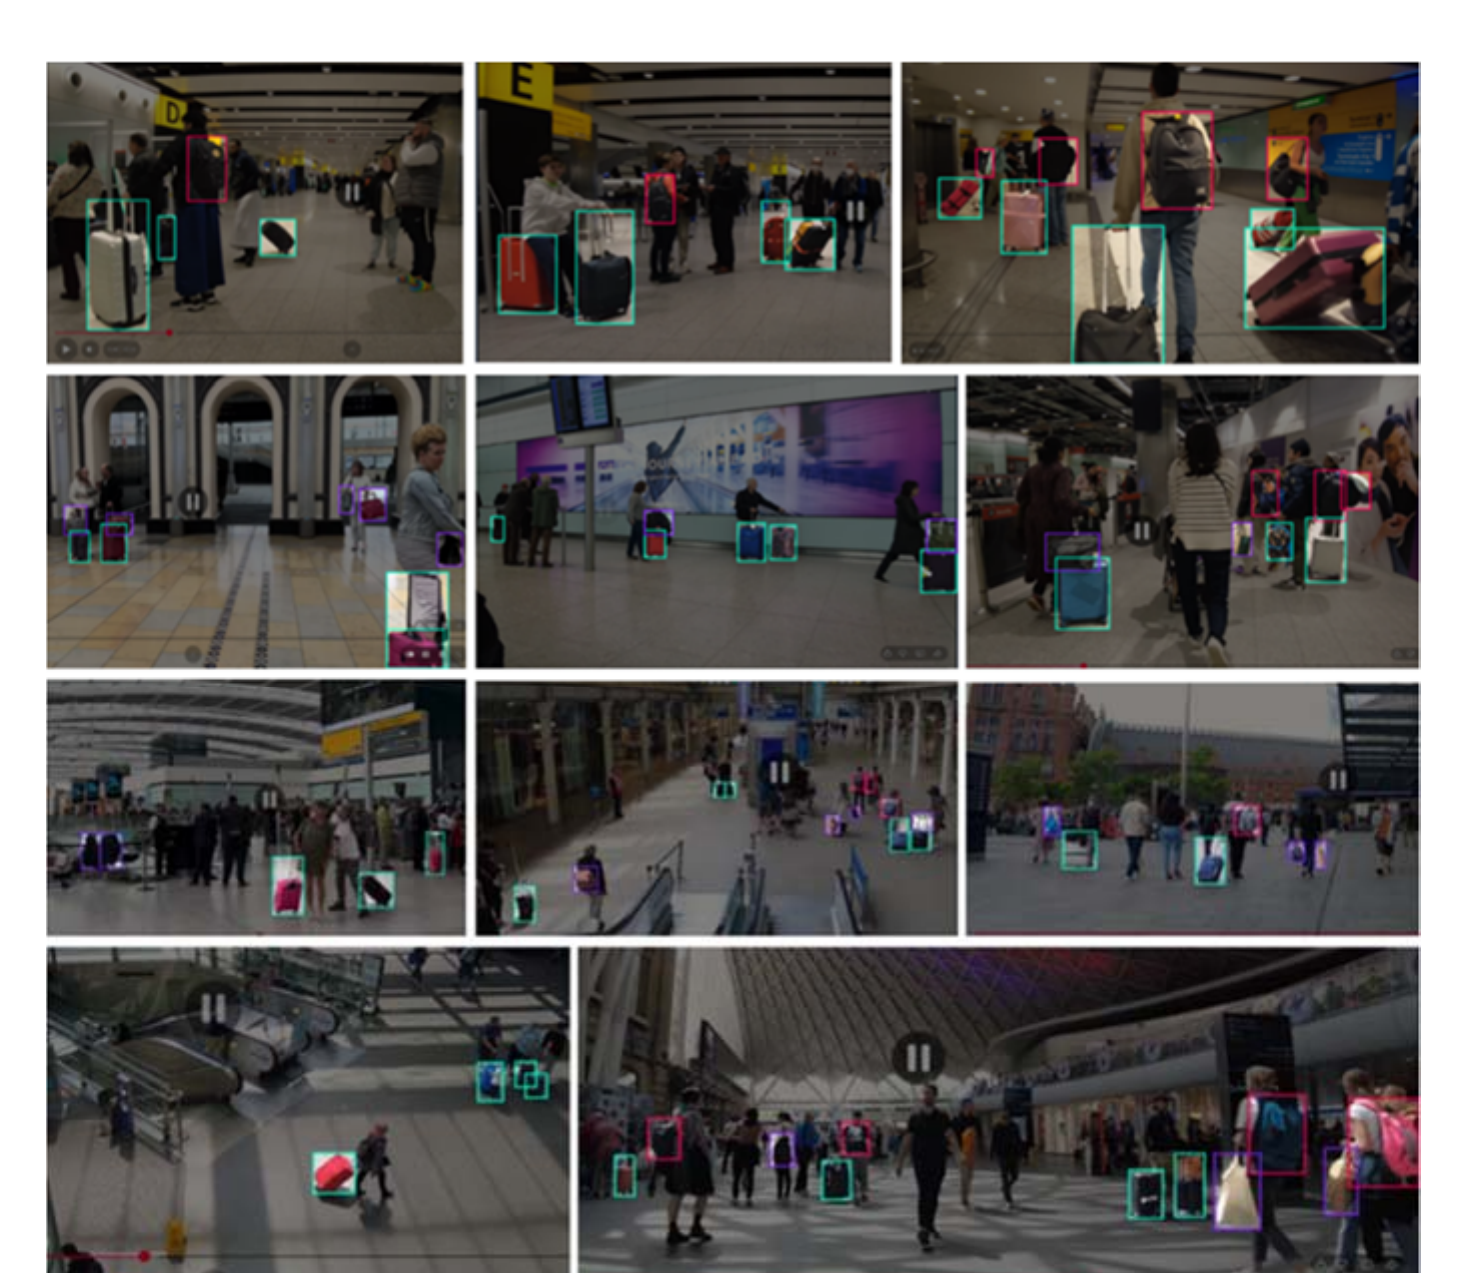
\includegraphics[width=\linewidth]{fig_samples.png}
\caption{Representative annotated frames from LuggageDataset~v6i. The images are
drawn from fixed or quasi-static surveillance cameras in transport hubs and
indoor public space, and illustrate the conditions the benchmark is built to
capture: elevated, oblique viewpoints in which luggage occupies a small fraction
of the frame; dense pedestrian traffic with frequent partial occlusion of the
bag by its own owner; wide variation in illumination, from daylit concourses to
artificially lit interiors and screen-lit walls; and all three classes
co-occurring at very different apparent scales within a single frame. The
annotations shown are the released ground truth. Note that these are the raw
frames: unlike our earlier presentation of this corpus, no augmentation is
applied anywhere in this paper, so every number reported in
Section~\ref{sec:results} is obtained on unmodified imagery.}
\label{fig:samples}
\end{figure}


\subsection{This Is a Small-Object Benchmark}

The mean annotated box measures $39\times55$~px in a 640-px frame, occupying
0.53\% of the image area. Table~\ref{tab:sizes} reports the size distribution
under two max-side conventions.

\begin{table}[t]
\centering
\caption{Object-size distribution, maximum bounding-box side, $32$ / $64$~px
edges. Counts are instances; percentages are row-wise, i.e.\ of that split or of
that class. The per-class rows cover the training split and sum to the Train
row; per-class totals are in Table~\ref{tab:shape}.}
\label{tab:sizes}
\small
\begin{tabular}{@{}lrrrrrr@{}}
\toprule
& \multicolumn{2}{c}{\textbf{Small} ($<$32)} & \multicolumn{2}{c}{\textbf{Medium} (32--64)} & \multicolumn{2}{c}{\textbf{Large} ($>$64)} \\
\cmidrule(lr){2-3}\cmidrule(lr){4-5}\cmidrule(lr){6-7}
 & $n$ & \% & $n$ & \% & $n$ & \% \\
\midrule
\multicolumn{7}{@{}l}{\textit{By split}}\\
Train & 14{,}959 & \textbf{35.8} & 16{,}398 & 39.2 & 10{,}466 & 25.0 \\
Valid & 3{,}669  & \textbf{37.4} & 4{,}034  & 41.1 & 2{,}116  & 21.6 \\
Test  & 2{,}175  & \textbf{35.2} & 2{,}510  & 40.7 & 1{,}487  & 24.1 \\
\addlinespace
\multicolumn{7}{@{}l}{\textit{By class, training split}}\\
backpack & 3{,}699 & 32.6 & 4{,}600 & \textbf{40.6} & 3{,}039 & 26.8 \\
bag      & 3{,}499 & \textbf{37.8} & 3{,}267 & \textbf{35.3} & 2{,}502 & \textbf{27.0} \\
trolley  & 7{,}761 & 36.6 & 8{,}531 & 40.2 & 4{,}925 & \textbf{23.2} \\
\bottomrule
\end{tabular}
\end{table}

Under this convention $35.8\%$ of training instances are small and a further
$39.2\%$ are medium. The choice
of \emph{maximum side} rather than area is deliberate: it is the side length, not
the area, that determines how many stride-8 feature cells a box spans, and
therefore how many anchors the label assigner can allocate to it---a quantity that
becomes central in Section~\ref{sec:method}.

\subsubsection*{Side length for the dataset, area for the metrics}

One clarification is needed before Section~\ref{sec:results}. The dataset
statistics above and every assignment diagnostic bin objects by \emph{maximum
side} at $32$ / $64$~px, because it is side length that determines anchor
supply. The reported detection metrics bin by \emph{area} at the COCO \cite{lin2014coco} edges
$1024$ / $9216$~px$^2$ --- equivalently $32^2$ / $96^2$ --- because that is what
the evaluator computes. Both are anchored at $32$~px, but they are not the same
partition: a $25\times100$ trolley has a maximum side of $100$~px yet an area of
only $2{,}500$~px$^2$, so it is large by side and medium by area. With $70.6\%$
of boxes taller than wide this is not a corner case, and we therefore state the
basis on every table and never compare a count against an AP across the two.

Unlike the closest comparable public set, v6i is not devoid of large objects:
10{,}466 training instances ($25.0\%$) exceed $64$~px on their longest side. This
matters because a benchmark with no large objects cannot measure whether a
small-object mechanism achieves its gains by sacrificing large ones---a trade-off
we observe repeatedly in Section~\ref{sec:results}.

\subsection{Boxes Are Tall, and the Classes Differ Sharply}

Across all splits, \textbf{70.6\%} of boxes are taller than wide
($h/w>1.25$), with a mean aspect ratio of 1.55 and only 6.0\% wide boxes. The
per-class breakdown in Table~\ref{tab:shape} shows that this aggregate conceals a
large difference between classes.

\begin{table}[t]
\centering
\caption{Per-class shape structure (training split). Size structure is in
Table~\ref{tab:sizes}; \texttt{bag} is the outlier on both.}
\label{tab:shape}
\footnotesize
\setlength{\tabcolsep}{3.5pt}
\begin{tabular}{@{}lrrrrr@{}}
\toprule
\textbf{Class} & \textbf{$n$} & \textbf{$h/w$} & \textbf{Wide} & \textbf{Square} & \textbf{Tall} \\
\midrule
backpack & 11{,}338 & 1.47 & 1.2\% & 23.8\% & \textbf{74.9\%} \\
bag      & 9{,}268  & \textbf{1.33} & \textbf{13.2\%} & \textbf{36.0\%} & 50.8\% \\
trolley  & 21{,}217 & \textbf{1.68} & 5.5\% & 17.6\% & \textbf{76.9\%} \\
\bottomrule
\end{tabular}
\end{table}

\texttt{trolley} is visually canonical: 76.9\% tall, mean ratio 1.68.
\texttt{bag}, by contrast, holds \textbf{48.5\% of every wide box in the dataset}
while representing only 22.2\% of instances, and is the only class whose three
shape bins are anywhere near balanced. Table~\ref{tab:sizes} shows it is also
the only class with a depleted size middle---simultaneously the highest large
share ($27.0\%$) and the lowest medium share ($35.3\%$), against a
\texttt{trolley} that is the most size-concentrated of the three. A class that
is at once the widest, the most balanced in shape and the most bimodal in size
is the one a single-scale prior fits worst, which is what
Section~\ref{sec:results:perclass} observes: \texttt{bag} is the hardest class
at every size on both detectors.

This heterogeneity is not incidental. \texttt{bag} is the weakest class by a wide
margin (AP$_{50\text{--}95}$ 0.4666 against \texttt{trolley}'s 0.6185, a 15.2-point
gap), and Section~\ref{sec:results} shows that this gap is attributable neither to
class frequency nor to assignment geometry nor to proposal failure. The category
is semantically loose---handbags, duffel bags, shopping bags, plastic bags---and
the residual gap is consistent with that looseness rather than with any
optimisation deficiency.

\subsection{A Leakage-Free Split}
\label{sec:dataset:leakage}

% =====================================================================
% The leakage-free splitting procedure. This is the original diagram from
% our weapon-detection paper (Catargiu & Ciocoiu, IEEE Access 2026),
% extracted from the published PDF. The procedure shown is the one applied
% unchanged to LuggageDataset v6i; the illustrative counts printed inside
% the panels are from the weapon corpus and are restated for v6i in the
% caption and in the accompanying text.
% =====================================================================
\begin{figure*}[t]
\centering
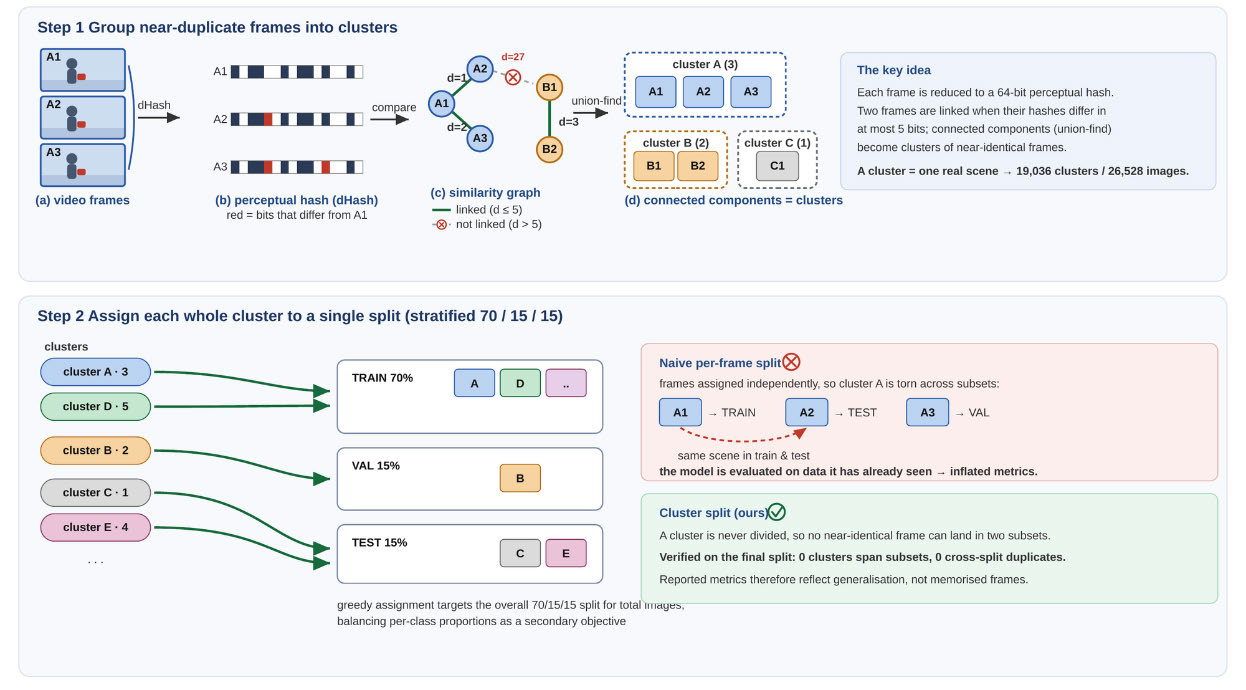
\includegraphics[width=\linewidth]{fig_leakage.png}
\caption{The leakage-free splitting procedure. \textbf{Step 1:} each frame is
reduced to a 64-bit perceptual (difference) hash; any two frames whose hashes
differ in at most five bits are linked, and connected components extracted by
union-find group mutually near-identical frames into clusters, so that one
cluster corresponds to one real scene. \textbf{Step 2:} each whole cluster,
never an individual frame, is assigned to a single split by a stratified greedy
procedure, so no near-duplicate frame can cross a split boundary by
construction. The panels illustrate the method with the counts from the
weapon-detection corpus in which it was first validated
\cite{catargiu2026weapon}; applied unchanged to LuggageDataset~v6i at the same
Hamming threshold of five, it produces the $75/15/10$ partition of
Table~\ref{tab:splits} and a cross-split audit of that partition returns
\textbf{zero} clusters spanning subsets and \textbf{zero} near-duplicate pairs
between any two subsets.}
\label{fig:leakage}
\end{figure*}


The corpus is assembled from surveillance video, and that single fact governs how
the split must be built. Consecutive frames of the same clip are near-identical:
the camera is fixed, the scene changes over seconds rather than frames, and the
same suitcase appears in hundreds of images that differ only by pedestrian
motion. A split that assigns \emph{frames} independently will therefore place the
same physical scene in both training and test, and the reported accuracy will
partly measure memorisation. This failure is invisible in the usual sanity
checks --- class proportions, image counts and size distributions all look
correct --- which is what makes it dangerous.

We therefore group before we split, following the procedure validated in our
earlier work on weapon detection \cite{catargiu2026weapon} and applied here
unchanged. Each image is reduced to a 64-bit difference hash. Any two images
whose hashes lie within a Hamming distance of $5$ are linked, and connected
components extracted by union-find collapse mutually near-identical frames into
clusters, so that \textbf{one cluster corresponds to one real scene}. The
threshold of $5$ follows common practice for difference-hash near-duplicate
detection: small enough to avoid merging visually distinct scenes, large enough
to capture frames that differ only by compression noise and small motion. Whole
clusters are then assigned to splits by a stratified greedy procedure that
targets the $75/15/10$ ratio on total image count and on each class
simultaneously. Because no cluster is ever divided, no near-duplicate frame can
cross a split boundary by construction.

A cross-split audit of the final partition confirms the guarantee holds in
practice: \textbf{zero clusters span more than one subset, and zero
near-duplicate pairs occur between any pair of subsets}. The evaluation is
therefore leakage-free, and the metrics in Section~\ref{sec:results} reflect
generalisation to unseen scenes rather than recall of frames the model has
already been trained on. Figure~\ref{fig:leakage} illustrates both steps and contrasts them with the
naive alternative; the counts printed inside its panels are those of the weapon
corpus in which the procedure was first validated, and the v6i figures are given
in Table~\ref{tab:splits}.

This matters for interpreting the size of our gains. The improvements reported in
this paper are $2$--$3\%$ relative. Had the split been built per frame, the
baseline itself would have scored higher --- and every mechanism would have
appeared to help less, because a memorising baseline leaves less headroom. A
leakage-free split is what makes a $+3.44\%$ gain meaningful rather than an
artefact of how the data was partitioned.

\subsection{Annotation Quality}

Automated label validation reports no out-of-range coordinates and no missing
label files. Two caveats are recorded for completeness. Two training images carry
labels that mix segmentation and detection rows and are rejected by the data
loader. Three duplicate labels are removed at load time (two in training, one in
validation), which is why the validation split yields 9{,}818 rather than 9{,}819
loaded instances.

\subsection{A Documented Split Drift}

Class proportions agree across splits to within 1.9 points and shape
distributions to within 0.8 points. One drift is material and we state it
explicitly: \textbf{the validation split under-represents large objects and
contains systematically smaller boxes than the test split}
(Table~\ref{tab:drift}).

\begin{table}[t]
\centering
\caption{Validation-split drift. Any threshold or hyperparameter tuned on
validation is tuned on a distribution with smaller objects than test.}
\label{tab:drift}
\small
\begin{tabular}{@{}lrrrr@{}}
\toprule
\textbf{Quantity} & \textbf{Train} & \textbf{Valid} & \textbf{Test} & \textbf{V vs T} \\
\midrule
Large share ($>$64 px) & 25.0\% & \textbf{21.6\%} & 24.1\% & $-$2.5 pt \\
Large count            & 10{,}466 & \textbf{2{,}116} & 1{,}487 & --- \\
Mean W $\times$ H (px) & 39$\times$55 & \textbf{35$\times$49} & 40$\times$56 & $-$23\% area \\
Boxes per image     & 4.58 & 5.37 & 5.06 & $+$6\% \\
\bottomrule
\end{tabular}
\end{table}

Validation boxes are approximately 23\% smaller in area than test boxes. Two
consequences follow. First, confidence thresholds tuned on validation are tuned
on a slightly harder, smaller-object distribution; we verify in
Section~\ref{sec:results} that the tuned operating point transfers to test intact,
but the drift bounds how far such tuning should be trusted. Second, any
large-object claim derived from validation alone rests on 758 instances against a
measured seed-to-seed spread of 2.11 points in the large bucket---we therefore
report all large-object results on test only.

\subsection{Comparison with Existing Benchmarks}

Against CCTV-KD, the largest annotated in-domain alternative
\cite{vrsalovic2025sensors}, v6i provides approximately \textbf{21$\times$ the
luggage annotations} (57{,}814 vs 2{,}760) from roughly \textbf{40$\times$ the
distinct source images} ($12{,}184$ vs $\sim$300 before augmentation), at three
class labels rather than one. Two differences favour CCTV-KD and we note them
plainly: it provides \texttt{person} annotations, which v6i does not, and its
scenes are considerably denser (approximately 20 annotated objects per image
against our 4.75). The absence of a person class means the ownership stage of our
pipeline must source person detections from a separate model, with the
domain-shift consequences discussed in Section~\ref{sec:method}.

Neither dataset contains abandonment events; both are detection benchmarks. v6i
is therefore complementary to ABODA and IITP20 rather than a replacement: it is
intended to train and evaluate the detector on which an event-level system is
built.

% =====================================================================
\section{Method}
\label{sec:method}

\begin{figure*}[t]
\centering
\iffigpng
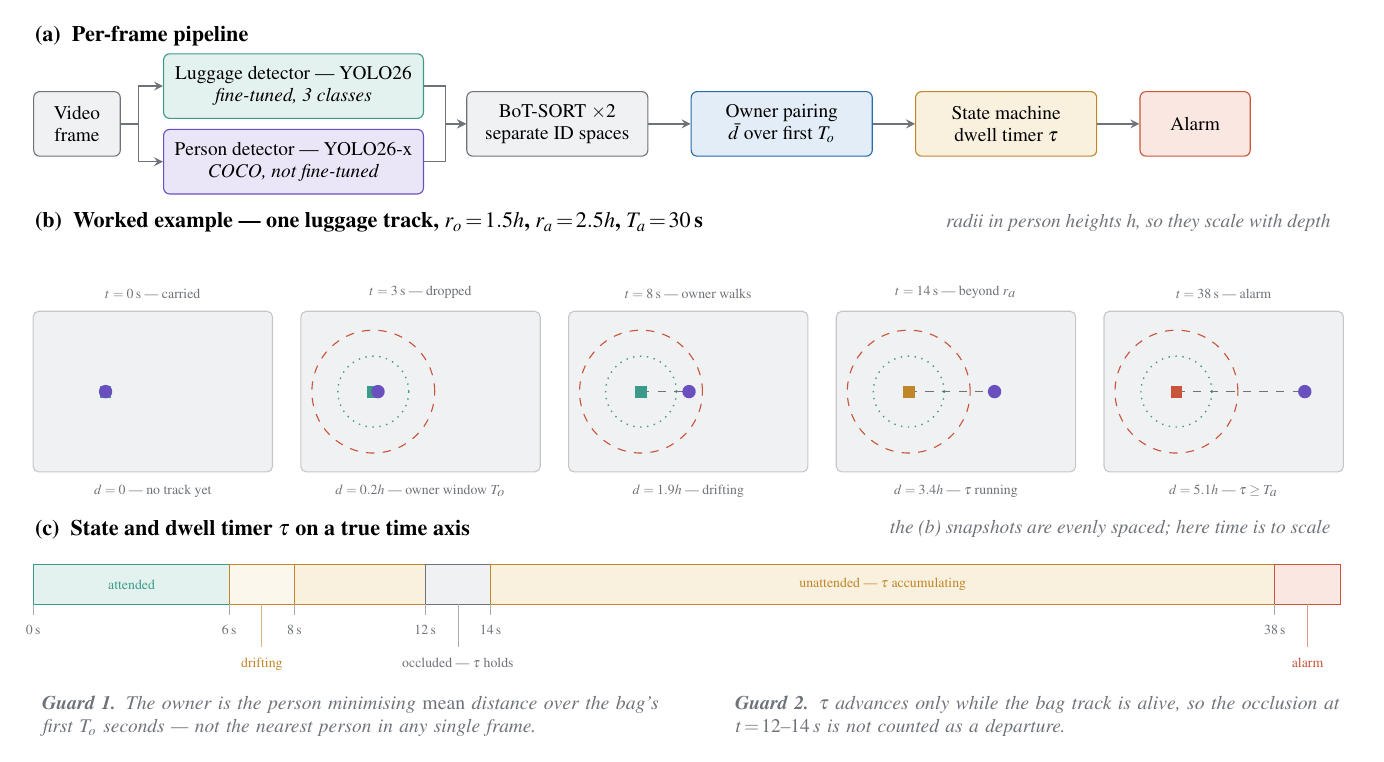
\includegraphics[width=\linewidth]{fig1.png}
\else
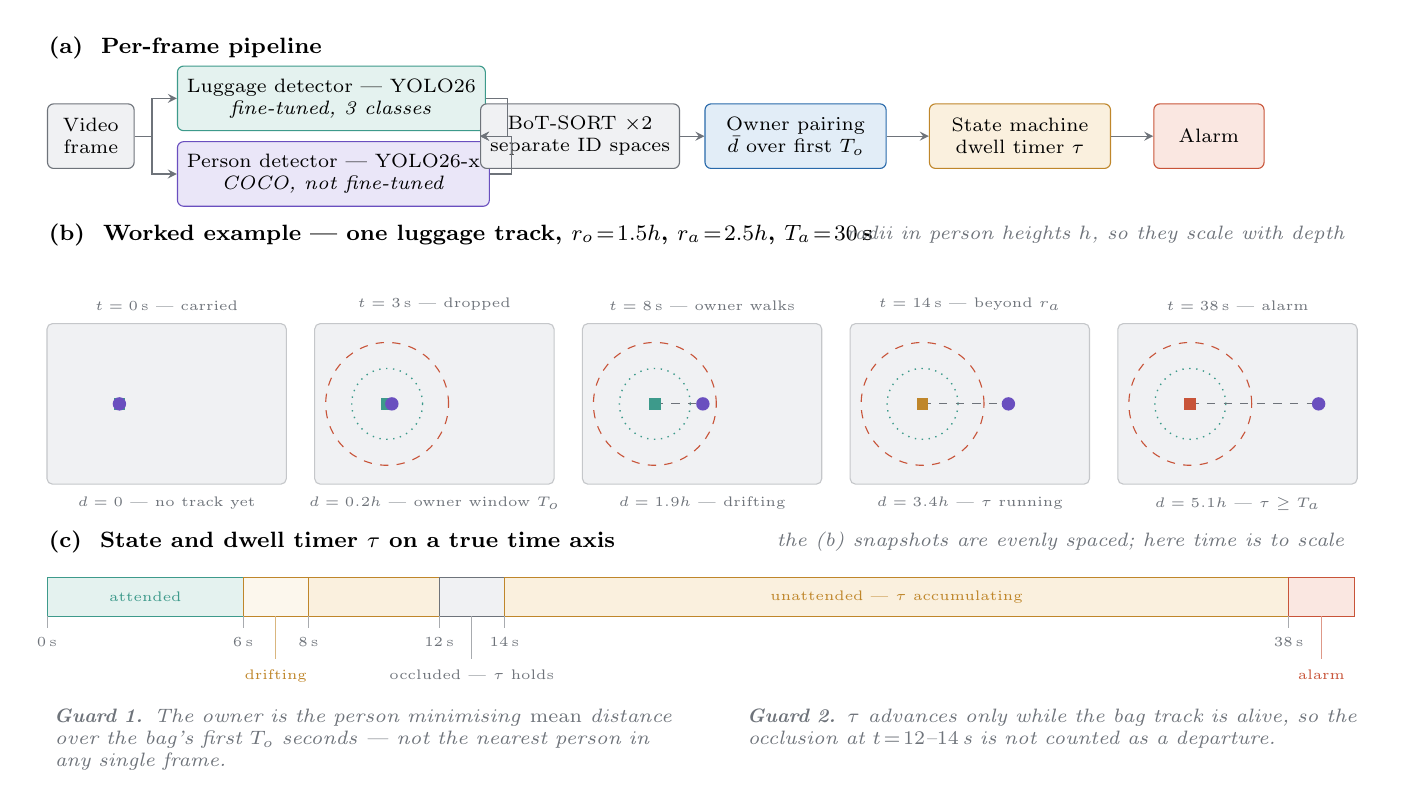
\begin{tikzpicture}[x=1cm,y=1cm]

%% ================= (a) pipeline =========================================
% Node widths are measured, not guessed: at \scriptsize the two detector
% boxes are 3.26 cm wide, so they must start far enough left of the tracker
% box that (dl.east) stays to the LEFT of (tr.west) -- otherwise the
% "-- ++(0.28,0) |- (tr.west)" connector doubles back on itself and draws a
% hook over the tracker box. Slots below are laid out with a 0.55 cm gap.
\node[font=\footnotesize\bfseries,anchor=west] at (0,2.22) {(a)~~Per-frame pipeline};

\node[blk,minimum width=11mm,anchor=west]  (fr) at (0.10,1.10) {Video\\frame};
\node[teal,minimum width=33mm,anchor=west] (dl) at (1.75,1.58) {Luggage detector \textemdash{} YOLO26\\\textit{fine-tuned, 3 classes}};
\node[purp,minimum width=33mm,anchor=west] (dp) at (1.75,0.62) {Person detector \textemdash{} YOLO26-x\\\textit{COCO, not fine-tuned}};
\node[blk,minimum width=23mm,anchor=west]  (tr) at (5.60,1.10) {BoT-SORT $\times2$\\separate ID spaces};
\node[blu,minimum width=23mm,anchor=west]  (op) at (8.45,1.10) {Owner pairing\\$\bar d$ over first $T_o$};
\node[amb,minimum width=23mm,anchor=west]  (sm) at (11.30,1.10) {State machine\\dwell timer $\tau$};
\node[cor,minimum width=14mm,anchor=west]  (al) at (14.15,1.10) {Alarm};

\draw[fl] (fr.east) -- ++(0.22,0) |- (dl.west);
\draw[fl] (fr.east) -- ++(0.22,0) |- (dp.west);
\draw[fl] (dl.east) -- ++(0.27,0) |- (tr.west);
\draw[fl] (dp.east) -- ++(0.27,0) |- (tr.west);
\draw[fl] (tr.east) -- (op.west);
\draw[fl] (op.east) -- (sm.west);
\draw[fl] (sm.east) -- (al.west);

%% ================= (b) worked example ===================================
\node[font=\footnotesize\bfseries,anchor=west] at (0,-0.15) {(b)~~Worked example \textemdash{} one luggage track, $r_o\!=\!1.5h$, $r_a\!=\!2.5h$, $T_a\!=\!30$\,s};
\node[lbl,anchor=east] at (16.70,-0.15) {radii in person heights $h$, so they scale with depth};

\def\sc#1#2#3#4#5#6{%
  \begin{scope}[shift={(#1,-2.30)}]
    \draw[draw=cGry!40,fill=cGryBg,rounded corners=2pt] (-1.52,-1.02) rectangle (1.52,1.02);
    \ifnum#6>0
      \draw[draw=cCor,dashed,line width=0.4pt] (-0.60,0) circle (0.78);
      \draw[draw=cTeal,dotted,line width=0.5pt] (-0.60,0) circle (0.45);
    \fi
    \ifnum#6>0 \draw[draw=cGry,line width=0.4pt,dashed] (-0.60,0) -- (#2,0); \fi
    \fill[#5] (-0.675,-0.075) rectangle (-0.525,0.075);
    \fill[cPurp] (#2,0) circle (0.085);
    \node[font=\tiny,text=cGry,anchor=south] at (0.0,1.06) {#3};
    \node[font=\tiny,text=cGry,anchor=north] at (0.0,-1.06) {#4};
  \end{scope}}

\sc{1.62}{-0.60}{$t=0$\,s \textemdash{} carried}{$d=0$ \textemdash{} no track yet}{cTeal}{0}
\sc{5.02}{-0.54}{$t=3$\,s \textemdash{} dropped}{$d=0.2h$ \textemdash{} owner window $T_o$}{cTeal}{1}
\sc{8.42}{0.01}{$t=8$\,s \textemdash{} owner walks}{$d=1.9h$ \textemdash{} drifting}{cTeal}{1}
\sc{11.82}{0.49}{$t=14$\,s \textemdash{} beyond $r_a$}{$d=3.4h$ \textemdash{} $\tau$ running}{cAmb}{1}
\sc{15.22}{1.03}{$t=38$\,s \textemdash{} alarm}{$d=5.1h$ \textemdash{} $\tau\ge T_a$}{cCor}{1}


%% ================= (c) timeline =========================================
% Time axis: x = 0.10 + 0.415*t, so 0 s -> 0.10, 6 -> 2.59, 8 -> 3.42,
% 12 -> 5.08, 14 -> 5.91, 38 -> 15.87, 40 -> 16.70.
% The bar is 0.50 cm tall (was 0.36) so the two inline labels sit clear of
% the rules, and ALL labels below it live on exactly two levels: timestamps
% at -5.16, segment names at -5.56. The vertical droplines that used to run
% down from the (b) snapshots are gone: the snapshots are evenly spaced but
% time is not, so those lines landed nowhere near their own timestamps.
\node[font=\footnotesize\bfseries,anchor=west] at (0,-4.05) {(c)~~State and dwell timer $\tau$ on a true time axis};
\node[lbl,anchor=east] at (16.70,-4.05) {the (b) snapshots are evenly spaced; here time is to scale};

\fill[cTealBg,draw=cTeal,line width=0.3pt]  (0.10,-5.00) rectangle (2.59,-4.50);
\fill[cAmbBg!55,draw=cAmb,line width=0.3pt] (2.59,-5.00) rectangle (3.42,-4.50);
\fill[cAmbBg,draw=cAmb,line width=0.3pt]    (3.42,-5.00) rectangle (5.08,-4.50);
\fill[cGryBg,draw=cGry,line width=0.3pt]    (5.08,-5.00) rectangle (5.91,-4.50);
\fill[cAmbBg,draw=cAmb,line width=0.3pt]    (5.91,-5.00) rectangle (15.87,-4.50);
\fill[cCorBg,draw=cCor,line width=0.3pt]    (15.87,-5.00) rectangle (16.70,-4.50);

\node[font=\tiny,text=cTeal] at (1.35,-4.75) {attended};
\node[font=\tiny,text=cAmb]  at (10.89,-4.75) {unattended \textemdash{} $\tau$ accumulating};

% level 1 -- timestamps, every event on one line
\foreach \x/\t in {0.10/0\,s, 2.59/6\,s, 3.42/8\,s, 5.08/12\,s, 5.91/14\,s, 15.87/38\,s}{
  \draw[draw=cGry!60,line width=0.3pt] (\x,-5.00) -- (\x,-5.14);
  \node[font=\tiny,text=cGry,anchor=north] at (\x,-5.14) {\t};}

% level 2 -- names of the segments too narrow to label inline
\draw[draw=cAmb!60,line width=0.3pt] (3.005,-5.00) -- (3.005,-5.54);
\node[font=\tiny,text=cAmb,anchor=north] at (3.005,-5.56) {drifting};
\draw[draw=cGry!60,line width=0.3pt] (5.495,-5.00) -- (5.495,-5.54);
\node[font=\tiny,text=cGry,anchor=north] at (5.495,-5.56) {occluded \textemdash{} $\tau$ holds};
\draw[draw=cCor!60,line width=0.3pt] (16.285,-5.00) -- (16.285,-5.54);
\node[font=\tiny,text=cCor,anchor=north] at (16.285,-5.56) {alarm};

%% ================= guards ==============================================
\node[lbl,anchor=north west,align=left,text width=79mm] at (0.10,-6.05)
 {\textbf{Guard 1.} The owner is the person minimising \emph{mean} distance over the
  bag's first $T_o$ seconds \textemdash{} not the nearest person in any single frame.};
\node[lbl,anchor=north west,align=left,text width=79mm] at (8.90,-6.05)
 {\textbf{Guard 2.} $\tau$ advances only while the bag track is alive, so the
  occlusion at $t\!=\!12$--$14$\,s is not counted as a departure.};

\end{tikzpicture}
\fi
\caption{The unattended-luggage pipeline and a worked example.
(a)~Two detectors run in parallel on every frame and are tracked independently,
so luggage and person identities never share an ID space. Only the luggage
detector is fine-tuned on our data; the person detector is a COCO model, which is
the weakest link in the chain (Section~\ref{sec:method}).
(b)~Top-down snapshots of a single track. The dotted inner circle is the
ownership radius $r_o$ and the dashed outer circle the alarm radius $r_a$, both
expressed in person heights $h$ so they scale with depth; the square is the bag
and the disc its assigned owner. The bag changes colour as the state advances.
(c)~The same episode on a time axis. The owner crosses $r_o$ at $6$\,s and $r_a$
at $8$\,s, at which point the dwell timer $\tau$ starts; it holds through the
occlusion at $12$--$14$\,s and reaches $T_a$ at $38$\,s.}
\label{fig:pipeline}
\end{figure*}

% =====================================================================
\subsection{Overview and Design Principle}
\label{sec:method:overview}

We modify two detectors --- YOLOv12s \cite{tian2025yolov12} and YOLO26s, both in
the Ultralytics implementation \cite{ultralytics} --- along two orthogonal axes. The \emph{loss axis} changes
how ground truth is assigned to anchors and how each assignment is weighted; the
\emph{architecture axis} changes which feature levels exist and how much capacity
each receives. Every modification obeys one rule: \textbf{at initialisation the
modified network must reproduce the pretrained baseline exactly}. Architectural
blocks are appended as residual branches with a zero-initialised gate, and loss
modifications reduce to the stock objective at their default parameter values.
This makes every comparison a controlled one---the pretrained weights transfer
without loss, and any difference in the final metric is attributable to the
mechanism rather than to a different initialisation.

The two detectors receive \emph{different} treatments, and this is a result
rather than an oversight. Superficially their objectives are the same: both use
BCE classification, CIoU \cite{zheng2020ciou} box regression, a task-aligned assigner with
$\alpha=0.5$ and $\beta=6$, and identical loss gains
($\mathrm{box}=7.5$, $\mathrm{cls}=0.5$, $\mathrm{dfl}=1.5$). Underneath they
differ in three respects that Table~\ref{tab:implsdiff} sets out and
Section~\ref{sec:disc:why} shows to be decisive: YOLOv12 regresses boxes as a
$16$-bin distribution and removes duplicates with NMS, whereas YOLO26 regresses
offsets directly ($\mathrm{reg\_max}=1$, with the third loss term becoming an
image-normalised $\ell_1$), runs \emph{two} assigners --- one-to-many and
one-to-one --- under a schedule that shifts weight from the former to the latter
across training, and emits a single prediction per object without NMS. As
Section~\ref{sec:results} shows, the mechanism that works on one does not work on
the other, in either direction.

% ---------------------------------------------------------------------
\subsection{Small-Object--Aware Loss and Assignment}
\label{sec:method:loss}

\subsubsection{Curriculum Area Weighting (YOLOv12)}

\emph{The problem.} After assignment, the regression loss sums over positives
with each weighted by its target score. Two things then work against small
objects at once. First, a large box collects far more positives than a small one
--- $9.79$ against $7.73$ on this dataset, from a candidate pool $51\times$
larger --- so it contributes more terms to the sum. Second, and more importantly,
the IoU term of a large box is smoothly informative: a few pixels of error
change its IoU very little, so its gradient is stable and well-scaled. For a
$12\times18$\,px bag the same few pixels can move IoU by tens of points. The
optimiser sees a loud, noisy signal from small objects and a quiet, reliable one
from large objects, and it does what any optimiser does --- it fits the reliable
signal first and treats the small objects as noise to be averaged out.

\emph{The intervention.} We restore the balance by weighting each positive by
the \emph{inverse linear scale} of its box, and we do so on a schedule rather
than permanently. Early in training, when the representation is still forming and
the small objects would otherwise never get a foothold, the weighting is
area-dominant; by the end it has decayed back to the standard score weighting,
so the final epochs optimise the objective the model is actually evaluated on.
This is the dynamic curriculum weighting introduced in our earlier work on
weapon detection \cite{catargiu2026weapon}. For each positive assignment $j$,

\begin{equation}
w_j^{(t)} = \alpha(t)\,\hat{a}_j + \bigl(1-\alpha(t)\bigr)\,s_j ,
\label{eq:swa}
\end{equation}

\noindent where $s_j$ is the summed target score of positive $j$ and $\hat a_j$
is a normalised, boosted inverse-scale term. Writing $A_j$ for the assigned box
area \emph{in feature units} at the level to which the anchor belongs, i.e.\
after division by that level's stride $\sigma_j$,

\begin{equation}
a_j = A_j^{-1/2},
\qquad
\hat a_j = \frac{a_j}{\max_{k \in \mathcal{P}} a_k}\; \cdot \; b_j ,
\label{eq:invarea}
\end{equation}

\noindent with $\mathcal{P}$ the set of positives in the batch. The exponent
$-\tfrac12$ makes the term scale with linear object size rather than with area;
a pure inverse-area weighting ($a_j = A_j^{-1}$) was also implemented and was
inferior on this dataset. The factor $b_j$ is a threshold boost applied after
normalisation,

\begin{equation}
b_j =
\begin{cases}
\rho, & \sqrt{A_j}\,\sigma_j < p_{\text{small}} \\
1, & \text{otherwise,}
\end{cases}
\label{eq:boost}
\end{equation}

\noindent which multiplies the weight of any positive whose box is smaller than
$p_{\text{small}}$ pixels on a side. The mixing coefficient follows a linear
curriculum over the $T$ training epochs, clipped to a fixed interval,

\begin{equation}
\alpha(t) = \mathrm{clip}\left(
\alpha_{\text{s}} \left(1 - t/T\right) + \alpha_{\text{e}}\, t/T,
\;\alpha_{\min},\; \alpha_{\max} \right),
\label{eq:curriculum}
\end{equation}

\noindent so optimisation begins scale-dominant, favouring small objects while
the representation is still forming, and ends score-balanced. The weight
$w_j^{(t)}$ multiplies the CIoU and DFL terms; the classification term is
untouched. With $\alpha_{\text{s}} = \alpha_{\text{e}} = 0$ the expression
reduces exactly to the stock per-positive weight $s_j$, which is the identity
property required in Section~\ref{sec:method:overview}. A grid search on the
validation split over $\alpha_{\text{s}} \in [0.6,0.9]$, $\alpha_{\text{e}} \in
[0.3,0.4]$, $p_{\text{small}} \in [36,48]$\,px and $\rho \in [1.0,2.5]$ selected
$\alpha_{\text{s}} = 0.7$, $\alpha_{\text{e}} = 0.3$, $p_{\text{small}} = 48$\,px
and $\rho = 2.0$; the full intervals are in Table~\ref{tab:search}.

Two design choices deserve comment. The exponent is $-\tfrac12$ rather than $-1$
because pure inverse-\emph{area} weighting is too aggressive on this data: with
boxes spanning three orders of magnitude in area, $A^{-1}$ makes the smallest
instances dominate the batch entirely and destabilises training, whereas
$A^{-1/2}$ scales with linear size and keeps the ratio bounded. Both were
implemented and the square root was better. The threshold boost of
Equation~\eqref{eq:boost} is then a blunt instrument layered on top: the
continuous term already up-weights small objects, but it does so smoothly, and
$48$\,px is the point below which this dataset's instances stop being resolvable
at stride $8$ at all. Doubling their weight is a statement that those specific
instances matter operationally, not a claim that the continuous weighting was
mis-shaped.

\subsubsection{Task-Alignment Exponents (YOLO26)}

The Task-Aligned Assigner \cite{tood2021} scores each (ground truth, anchor) pair by

\begin{equation}
m_{ij} = s_{ij}^{\,\alpha}\;\cdot\;u_{ij}^{\,\beta},
\label{eq:align}
\end{equation}

\noindent where $s_{ij}$ is the predicted class score for the ground-truth
class and $u_{ij}$ the IoU. Both detectors construct their assigners with
$\alpha = 0.5$ and $\beta = 6$; these are fixed constants in the reference
implementation and are not exposed as tunable hyperparameters. We exposed both
and swept them.

The metric enters the objective at three distinct points, and it is essential to
separate them. First, \emph{selection}: the $k$ anchors with the largest
$m_{ij}$ inside each ground-truth box become positives. Second, \emph{tie-break}
in the one-to-one branch, where $k=1$. Third, \emph{target magnitude}: the
classification target of a positive is not $1$ but

\begin{equation}
\hat{t}_{ij}
= \frac{m_{ij}\;\max_{j' \in \mathcal{P}_i} u_{ij'}}
       {\max_{j' \in \mathcal{P}_i} m_{ij'} + \epsilon},
\label{eq:normalign}
\end{equation}

\noindent so a well-aligned anchor is asked for a higher confidence than a
poorly aligned one. Equation~\eqref{eq:normalign} carries a consequence we use
in Section~\ref{sec:discussion}: when a ground truth has exactly one positive
--- which is the case in YOLO26's one-to-one branch --- the ratio is identically
$1$ and the target collapses to $\max u$, so $\alpha$ and $\beta$ \emph{provably
cannot} change the target magnitude on that branch. They can only change
\emph{which} anchor receives it.

\emph{Our modification is a single exponent}, $\beta: 6 \rightarrow 1$, selected from
nine values spanning $[0,6]$ (Table~\ref{tab:search}). The
reason it should matter is a statement about how IoU behaves at different
scales. Consider two anchors on a large object whose IoUs are $0.80$ and $0.70$.
Raised to the sixth power these become $0.262$ and $0.118$ --- the assigner
treats the first as more than twice as good, and it is right to, because on a
large box a $0.10$ IoU gap is a real and stable difference in localisation.
Now consider the same gap on a $12\times18$\,px bag. There, one pixel of
displacement moves IoU by several points, so a $0.80$ versus $0.70$ split
between two neighbouring anchors is mostly sampling noise --- yet $\beta=6$
still amplifies it into a factor of $2.2$ in the alignment metric, and
Equation~\eqref{eq:normalign} then propagates that amplified difference into the
classification target the model is asked to reproduce.

Setting $\beta=1$ makes the metric linear in IoU. The ranking is preserved ---
better-localised anchors still win --- but the \emph{margins} are compressed, so
the assigner stops manufacturing confident distinctions between anchors that are
in truth equally good. The prediction is therefore specific: reducing $\beta$
should help most where IoU is noisiest, which is exactly the small-object regime,
and should be roughly neutral elsewhere. Section~\ref{sec:results} reports that
the loss axis helps on small objects while costing mAP$_{50\text{-}95}$
($-0.35\%$ on YOLO26 and $-0.37\%$ on YOLOv12) --- the metric that rewards
precisely the fine localisation distinctions a large $\beta$ was amplifying.

\subsubsection{Anchor Supply and Why the Effect Is Bounded}

Both mechanisms above act on assignments that already exist. Whether they
\emph{can} act is a question about anchor supply. For a box of size $w \times h$
at feature stride $s$, the number of anchor centres falling inside it is

\begin{equation}
n(s) = \left[ \lfloor x_2/s - 1/2 \rfloor - \lceil x_1/s - 1/2 \rceil + 1 \right]_+
\;\cdot\;
\left[ \lfloor y_2/s - 1/2 \rfloor - \lceil y_1/s - 1/2 \rceil + 1 \right]_+ ,
\label{eq:footprint}
\end{equation}

\noindent summed over the levels of the pyramid, where $[\cdot]_+$ denotes
$\max(\cdot,0)$ and indices are additionally clamped to the feature map, which
we omit here as it affects only boxes touching the image border. Measured over the training
labels, a small luggage instance commands $12.90$ anchor centres in total
($9.82$ at stride $8$, $2.46$ at $16$, $0.62$ at $32$) against a selection
budget of $k=10$, while a large instance commands $657.67$ --- a supply ratio of
$51\times$. Standard assignment converts $7.73$ of the small object's $12.90$
candidates into positives, i.e.\ $60\%$ of its entire pool.

The budget is therefore close to \emph{slack}. Of small ground truths,
$38$--$42\%$ hold fewer than $k$ centres at evaluation geometry, and once mosaic
augmentation halves the effective scale --- which it does for $60$ of the $70$
training epochs --- that figure rises to approximately $70\%$. For those
instances every candidate is already a positive, the ranking cannot change the
assignment, and the selection role of Equation~\eqref{eq:align} is inert; only
its target-magnitude role acts. Adding a stride-$4$ level multiplies the finest
level's count by four and raises the small object's pool to roughly $52$
centres, which makes $k$ binding again. This is the diagnostic that motivates
the architectural axis, and Section~\ref{sec:results} reports that its central
prediction was refuted on one detector and only weakly supported on the other.

The same table motivates the level reallocation of
Section~\ref{sec:method:arch}. At stride $32$ a small object draws $0.01$
positives per ground truth and a medium object $0.00$, against pools of $0.62$
and $2.71$: the few candidates that exist carry an alignment metric near zero
and fail the positivity test regardless of budget. Large objects draw $7.96$ of
their $9.79$ positives ($81\%$) from stride $16$, not stride $32$. The coarsest
detection level is thus doing very little work on this dataset.

% ---------------------------------------------------------------------
\subsection{Architectural Modifications}
\label{sec:method:arch}

% =====================================================================
% FIGURE 2 — the two architectural modifications.
% Layout convention: the VERTICAL axis is the pyramid level (P5/32 at the
% top, P2/4 at the bottom) and the HORIZONTAL axis is depth through the
% network. Every edge is transcribed from the `from` field of the YAML;
% Conv-downsample and Concat rows are folded into the edge LABELS so that
% only tensor-producing blocks appear as boxes.
%
%   (a) BACKBONE + HEAD_DYSAMPLE + TAIL_LS_SHIFT  (run_arch_port_v6i.py)
%       9<-8  11<-[9,6]  12<-11  14<-[12,4]  17<-[15,11]  20<-[19,8]
%       21<-14  23<-[21,2]  24<-23  25<-14  26<-17  27<-20  28<-[24..27]
%   (b) yolo26-p2dys-p234rich.yaml
%       13<-[11,6]  16<-[14,4]  17<-16  19<-[17,2]  22<-[20,16]
%       25<-[23,13]  26<-[19,22,25]
% =====================================================================
\begin{figure*}[t]
\centering
\iffigpng
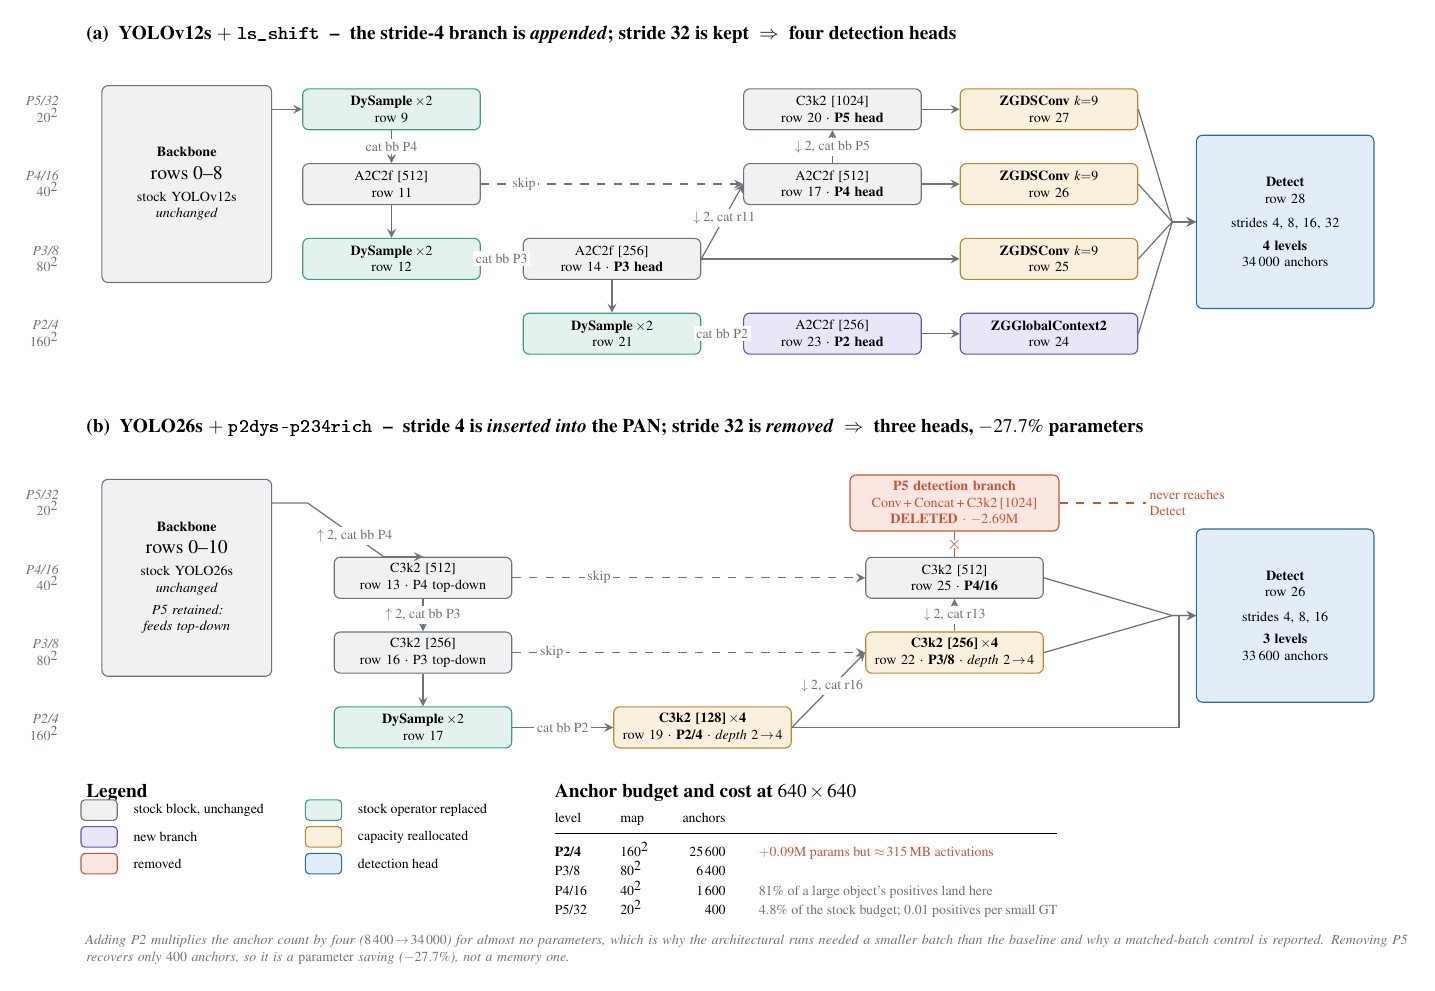
\includegraphics[width=\linewidth]{fig2.png}
\else
\begin{tikzpicture}[x=1cm,y=1cm,
  nd/.style={blk,minimum height=5.2mm,inner sep=2.2pt,font=\tiny,text width=21mm},
  hd/.style={font=\scriptsize\bfseries,align=left},
  el/.style={font=\tiny,text=cGry,fill=white,inner sep=1pt},
  lv/.style={font=\tiny\itshape,text=cGry,anchor=east,align=right},
  strk/.style={nd,draw=cCor,fill=cCorBg,text=cCor},
]
\def\LV{-0.60} \def\LIV{-1.55} \def\LIII{-2.50} \def\LII{-3.45}

% =====================================================================
% (a) YOLOv12s + ls_shift
% =====================================================================
\node[hd,anchor=west] at (0.15,0.35) {(a)~~YOLOv12s\;$+$\;\texttt{ls\_shift} \;--\; the stride-4 branch is \emph{appended}; stride 32 is kept \;$\Rightarrow$\; four detection heads};

\node[lv] at (0.05,\LV)   {P5/32\\$20^2$};  \node[lv] at (0.05,\LIV) {P4/16\\$40^2$};
\node[lv] at (0.05,\LIII) {P3/8\\$80^2$};   \node[lv] at (0.05,\LII) {P2/4\\$160^2$};

\node[nd,fill=cGryBg,draw=cGry,minimum height=25mm,text width=20mm] (a_bb) at (1.55,\LIV)
  {\textbf{Backbone}\\\scriptsize rows 0--8\\[2pt]\tiny stock YOLOv12s\\\tiny\emph{unchanged}};

\node[nd,draw=cTeal,fill=cTealBg] (a9)  at (4.15,\LV)   {\textbf{DySample}\,$\times2$\\\tiny row 9};
\node[nd]                          (a11) at (4.15,\LIV)  {A2C2f [512]\\\tiny row 11};
\node[nd,draw=cTeal,fill=cTealBg] (a12) at (4.15,\LIII) {\textbf{DySample}\,$\times2$\\\tiny row 12};

\node[nd]                          (a14) at (6.95,\LIII) {A2C2f [256]\\\tiny row 14 · \textbf{P3 head}};
\node[nd,draw=cTeal,fill=cTealBg] (a21) at (6.95,\LII)  {\textbf{DySample}\,$\times2$\\\tiny row 21};

\node[nd]                          (a20) at (9.75,\LV)   {C3k2 [1024]\\\tiny row 20 · \textbf{P5 head}};
\node[nd]                          (a17) at (9.75,\LIV)  {A2C2f [512]\\\tiny row 17 · \textbf{P4 head}};
\node[nd,draw=cPurp,fill=cPurpBg] (a23) at (9.75,\LII)  {A2C2f [256]\\\tiny row 23 · \textbf{P2 head}};

\node[nd,draw=cAmb,fill=cAmbBg]   (a27) at (12.5,\LV)   {\textbf{ZGDSConv} $k{=}9$\\\tiny row 27};
\node[nd,draw=cAmb,fill=cAmbBg]   (a26) at (12.5,\LIV)  {\textbf{ZGDSConv} $k{=}9$\\\tiny row 26};
\node[nd,draw=cAmb,fill=cAmbBg]   (a25) at (12.5,\LIII) {\textbf{ZGDSConv} $k{=}9$\\\tiny row 25};
\node[nd,draw=cPurp,fill=cPurpBg] (a24) at (12.5,\LII)  {\textbf{ZGGlobalContext2}\\\tiny row 24};

\node[nd,draw=cBlu,fill=cBluBg,minimum height=22mm,text width=21mm] (adet) at (15.5,\LIII+0.47)
  {\textbf{Detect}\\\tiny row 28\\[3pt]\tiny strides 4, 8, 16, 32\\[2pt]\tiny\textbf{4 levels}\\\tiny 34\,000 anchors};

% --- true edges ---
\draw[fl] (a_bb.east|-a9) -- (a9.west);
\draw[fl] (a9.south)  -- node[el]{cat bb P4} (a11.north);
\draw[fl] (a11.south) -- (a12.north);
\draw[fl] (a12.east)  -- node[el]{cat bb P3} (a14.west);
\draw[fl] (a14.east)  -- node[el,pos=0.55]{$\downarrow2$, cat r11} (a17.west);
\draw[fl] (a17.north) -- node[el]{$\downarrow2$, cat bb P5} (a20.south);
\draw[fl] (a14.south) -- (a21.north);
\draw[fl] (a21.east)  -- node[el]{cat bb P2} (a23.west);
\draw[flb] (a11.east) -- ++(0.55,0) |- node[el,pos=0.28]{skip} (a17.west);
\draw[fl] (a20.east) -- (a27.west);
\draw[fl] (a17.east) -- (a26.west);
\draw[fl] (a14.east) -- ++(0.35,0) -- ($(a25.west)+(-0.35,0)$) -- (a25.west);
\draw[fl] (a23.east) -- (a24.west);
\foreach \s in {a24,a25,a26,a27} \draw[fl] (\s.east) -- ($(adet.west)+(-0.3,0)$) -- (adet.west);

% =====================================================================
% (b) YOLO26s + p2dys-p234rich
% =====================================================================
\begin{scope}[yshift=-5.0cm]
\node[hd,anchor=west] at (0.15,0.35) {(b)~~YOLO26s\;$+$\;\texttt{p2dys-p234rich} \;--\; stride 4 is \emph{inserted into} the PAN; stride 32 is \emph{removed} \;$\Rightarrow$\; three heads, $-27.7\%$ parameters};

\node[lv] at (0.05,\LV)   {P5/32\\$20^2$};  \node[lv] at (0.05,\LIV) {P4/16\\$40^2$};
\node[lv] at (0.05,\LIII) {P3/8\\$80^2$};   \node[lv] at (0.05,\LII) {P2/4\\$160^2$};

\node[nd,fill=cGryBg,draw=cGry,minimum height=25mm,text width=20mm] (b_bb) at (1.55,\LIV)
  {\textbf{Backbone}\\\scriptsize rows 0--10\\[2pt]\tiny stock YOLO26s\\\tiny\emph{unchanged}\\[2pt]\tiny\emph{P5 retained:}\\\tiny\emph{feeds top-down}};

\node[nd]                          (b13) at (4.55,\LIV)  {C3k2 [512]\\\tiny row 13 · P4 top-down};
\node[nd]                          (b16) at (4.55,\LIII) {C3k2 [256]\\\tiny row 16 · P3 top-down};
\node[nd,draw=cTeal,fill=cTealBg] (b17) at (4.55,\LII)  {\textbf{DySample}\,$\times2$\\\tiny row 17};

\node[nd,draw=cAmb,fill=cAmbBg]   (b19) at (8.10,\LII)  {\textbf{C3k2 [128]}\,$\times\mathbf{4}$\\\tiny row 19 · \textbf{P2/4} · \emph{depth $2\!\to\!4$}};
\node[nd,draw=cAmb,fill=cAmbBg]   (b22) at (11.3,\LIII) {\textbf{C3k2 [256]}\,$\times\mathbf{4}$\\\tiny row 22 · \textbf{P3/8} · \emph{depth $2\!\to\!4$}};
\node[nd]                          (b25) at (11.3,\LIV)  {C3k2 [512]\\\tiny row 25 · \textbf{P4/16}};

\node[strk,text width=25mm]        (b5x) at (11.3,\LV)   {\textbf{P5 detection branch}\\\tiny Conv\,+\,Concat\,+\,C3k2\,[1024]\\\tiny\textbf{DELETED} · $-2.69$M};

\node[nd,draw=cBlu,fill=cBluBg,minimum height=22mm,text width=21mm] (bdet) at (15.5,\LIII+0.47)
  {\textbf{Detect}\\\tiny row 26\\[3pt]\tiny strides 4, 8, 16\\[2pt]\tiny\textbf{3 levels}\\\tiny 33\,600 anchors};

% --- true edges ---
% main path. NOTE: row 11 upsamples the BACKBONE P5 output (row 10), so this
% edge must leave the backbone at the P5 line, not at P4.
\draw[fl] (b_bb.east|-0,\LV) -- ++(0.45,0) -- node[el,pos=0.62]{$\uparrow2$, cat bb P4} ($(b13.north)+(-0.5,0)$) -- ($(b13.north)+(-0.5,0)$) -- (b13.north);
\draw[fl] (b13.south) -- node[el]{$\uparrow2$, cat bb P3} (b16.north);
\draw[fl] (b16.south) -- (b17.north);
\draw[fl] (b17.east)  -- node[el]{cat bb P2} (b19.west);
\draw[fl] (b19.east)  -- node[el,pos=0.55]{$\downarrow2$, cat r16} (b22.west);
\draw[fl] (b22.north) -- node[el]{$\downarrow2$, cat r13} (b25.south);
\draw[flb] (b16.east) -- ++(0.5,0) |- node[el,pos=0.3]{skip} (b22.west);
\draw[flb] (b13.east) -- ++(1.1,0) |- node[el,pos=0.3]{skip} (b25.west);
% row 19 routes BELOW rows 22/25 rather than clipping their labels
\draw[fl] (b19.east) -- ++(0.3,0) -- (14.15,\LII) -- (14.15,\LIII+0.47) -- (bdet.west);
\foreach \s in {b22,b25} \draw[fl] (\s.east) -- ($(bdet.west)+(-0.3,0)$) -- (bdet.west);
% the deleted branch, shown hanging off the P4 head where it used to attach
\draw[dashed,draw=cCor,line width=0.5pt] (b25.north) -- (b5x.south);
\node[text=cCor,font=\scriptsize\bfseries] at ($(b25.north)!0.5!(b5x.south)$) {$\times$};
\draw[dashed,draw=cCor,line width=0.5pt] (b5x.east) -- ++(1.1,0)
  node[el,text=cCor,right=0pt,align=left]{never reaches\\Detect};
\end{scope}

% =====================================================================
% (c) legend + the per-level budget that makes the cost visible
% =====================================================================
\begin{scope}[yshift=-9.05cm]
\node[anchor=north west,font=\scriptsize\bfseries] at (0.15,0) {Legend};
% swatches drawn as plain nodes: a tabular of nested \tikz pictures does not
% survive inside a tikz node, so the two columns are placed explicitly.
\foreach \i/\col/\bg/\txt in {0/cGry/cGryBg/{stock block, unchanged},
                              1/cPurp/cPurpBg/{new branch},
                              2/cCor/cCorBg/{removed}}{
  \node[draw=\col,fill=\bg,rounded corners=1.4pt,minimum width=4.6mm,minimum height=2.6mm,
        inner sep=0pt,anchor=west] at (0.20,-0.45-0.34*\i) {};
  \node[anchor=west,font=\tiny] at (0.75,-0.45-0.34*\i) {\txt};
}
\foreach \i/\col/\bg/\txt in {0/cTeal/cTealBg/{stock operator replaced},
                              1/cAmb/cAmbBg/{capacity reallocated},
                              2/cBlu/cBluBg/{detection head}}{
  \node[draw=\col,fill=\bg,rounded corners=1.4pt,minimum width=4.6mm,minimum height=2.6mm,
        inner sep=0pt,anchor=west] at (3.05,-0.45-0.34*\i) {};
  \node[anchor=west,font=\tiny] at (3.60,-0.45-0.34*\i) {\txt};
}

\node[anchor=north west,font=\scriptsize\bfseries] at (6.1,0) {Anchor budget and cost at $640\times640$};
\node[anchor=north west,font=\tiny] at (6.1,-0.34) {%
\begin{tabular}{@{}llrl@{}}
level & map & anchors & \\
\midrule
\textbf{P2/4}  & $160^2$ & $25\,600$ & \textcolor{cCor}{$+0.09$M params but $\approx\!315$\,MB activations} \\
P3/8           & $80^2$  & $6\,400$  & \\
P4/16          & $40^2$  & $1\,600$  & \textcolor{cGry}{$81\%$ of a large object's positives land here} \\
P5/32          & $20^2$  & $400$     & \textcolor{cGry}{$4.8\%$ of the stock budget; $0.01$ positives per small GT} \\
\end{tabular}};

\node[anchor=north west,font=\tiny\itshape,text=cGry,text width=168mm,align=left] at (0.15,-1.92)
 {Adding P2 multiplies the anchor count by four ($8\,400\!\to\!34\,000$) for almost no parameters, which is why the architectural runs
  needed a smaller batch than the baseline and why a matched-batch control is reported. Removing P5 recovers only $400$ anchors, so it is
  a \emph{parameter} saving ($-27.7\%$), not a memory one.};
\end{scope}

\end{tikzpicture}
\fi
\caption{The two architectural modifications. The vertical axis is the pyramid level and the horizontal axis is depth through the network; solid arrows are
the main data path, dashed arrows are lateral skips, and \texttt{Conv}-downsample and \texttt{Concat} rows are folded into the edge labels so that only
tensor-producing blocks are drawn. (a)~On YOLOv12s the stride-4 branch is \emph{appended}: the existing top-down/bottom-up path (rows 9--20) is left intact, a
P2 head is built from row 14 by content-aware upsampling, and each of the four levels then receives one gated refinement block --- global context where the
small objects are, a directional snake kernel where the medium and large ones are. (b)~On YOLO26s the stride-4 branch is \emph{inserted} into the PAN and the
bottom-up path is rebuilt through it (row 19 $\rightarrow$ 22 $\rightarrow$ 25), the two finest levels are deepened from two blocks to four, and the stride-32
\emph{detection} branch is deleted while the stride-32 backbone is retained to feed the top-down path. Every coloured block is gated as in
Eq.~\eqref{eq:gate}, so at initialisation both networks reproduce their pretrained baseline exactly. (c)~The anchor budget makes the asymmetry of the shared
change explicit: the stride-4 level supplies $75\%$ of all anchors for $0.09$M parameters but roughly $315$\,MB of activations, whereas stride 32 holds only
$4.8\%$ of the stock budget --- so adding P2 is a \emph{memory} cost and removing P5 is a \emph{parameter} saving, and the two do not offset.}
\label{fig:arch}
\end{figure*}


Figure~\ref{fig:arch} shows the two resulting graphs. They share one change ---
a stride-4 detection level --- and differ in everything built around it, which
is what makes the comparison in Section~\ref{sec:results:transfer} possible.

All blocks below are channel- and resolution-preserving, and each is applied as

\begin{equation}
y = x + \gamma \odot \mathcal{F}(x), \qquad \gamma \big|_{t=0} = 0,
\label{eq:gate}
\end{equation}

\noindent with $\gamma$ a learnable per-channel gate. At epoch $0$ the block is
the identity, so the pretrained detector is reproduced exactly and the transfer
is lossless.

\subsubsection{Content-Aware Upsampling}

The top-down path is rebuilt with DySample \cite{dysample2023} in place of
nearest-neighbour interpolation. Rather than replicating each feature, it
predicts per-location sampling offsets and gathers by bilinear interpolation,
\begin{equation}
y_p = x\bigl(p/\rho + \Delta_p\bigr), \qquad
\Delta_p = \tfrac{1}{2}\,\sigma\bigl(\mathcal{S}(x)\bigr) \odot \mathcal{O}(x) + p_0 ,
\label{eq:dysample}
\end{equation}
where $\rho$ is the scale factor, $\mathcal{O}$ the offset convolution,
$\mathcal{S}$ the dynamic-scope branch and $p_0$ the fixed initial sampling
grid. The scope branch is zero-initialised, so $\sigma(\mathcal{S}(x)) =
\tfrac12$ and the factor collapses to the static $0.25$ of the original
formulation; the offset convolution is near-zero initialised, so upsampling
begins equivalent to bilinear. This
matters most on the path feeding the finest level, where nearest-neighbour
upsampling blurs precisely the detail small luggage depends on.

\subsubsection{A Stride-4 Detection Level}

Both detectors receive a P2 branch at stride $4$: the finest existing pyramid
level is upsampled onto the stride-4 backbone feature and fused, adding a
detection head at $160\times160$.

This is the one change that addresses the supply problem of
Equation~\eqref{eq:footprint} directly rather than working around it. Every loss
mechanism in Section~\ref{sec:method:loss} redistributes weight among
assignments that already exist; none of them can create a positive where no
anchor centre falls. A stride-4 level does exactly that, quadrupling the finest
level's contribution and taking a small object's pool from $12.90$ centres to
roughly $52$. It is also the only change that improves the \emph{resolution} at
which a small object is represented, rather than the emphasis it receives.

The cost is asymmetric and worth stating precisely, because it shaped the
experimental design. The branch adds only $0.09$M parameters --- trivial --- but
roughly $315$\,MB of activation memory at batch $48$, since activation cost
scales with spatial area and a stride-4 map is sixteen times larger than a
stride-16 one. Anchors rise from $8{,}400$ to $34{,}000$. This is why
architectural runs were executed at a reduced batch size and why a matched-batch
control was measured rather than assumed (Section~\ref{sec:results:batch}), and
the configurations we report were retrained under a single protocol per detector
once the design was fixed.

\subsubsection{Level-Specific Refinement (YOLOv12)}

On YOLOv12 the P2 branch is \emph{appended}: rows 9--20 of the stock graph are
left untouched and the new head is built from row 14 (Fig.~\ref{fig:arch}a).
This choice is deliberate. It keeps the pretrained neck weights aligned by name,
so the transfer is exact and the only randomly initialised parameters are the
new branch, and it means the four-level model is the three-level model plus
something, which makes the ablation interpretable.

Each detection level then receives one gated block, matched to what that level
actually sees. At the stride-4 level we attach \textbf{ZGGlobalContext2}, which
forms a global descriptor from both average and maximum pooling and broadcasts
it back additively, in the spirit of global-context modelling \cite{cao2019gcnet}:
\begin{equation}
\mathcal{F}(x) = \mathrm{MLP}\left( \left[\; \overline{x} \;;\; \max\nolimits_{H,W} x \;\right] \right),
\label{eq:gctx}
\end{equation}
with $\overline{x}$ the spatial mean. The average branch supplies scene context;
the maximum branch preserves the single most salient activation, which is the
cue a small, rare instance produces and which averaging removes. At strides $8$,
$16$ and $32$ we attach \textbf{ZGDSConv}, a zero-gated dynamic snake
convolution \cite{qi2023dscnet}: two one-dimensional deformable branches, one
snaking along each axis, whose taps accumulate offsets outward from the centre,
\begin{equation}
\delta_{c+m} = \!\!\sum_{\iota=0}^{m}\! \tanh\bigl(o_{c+\iota}\bigr),
\qquad
\delta_{c-m} = -\!\!\sum_{\iota=1}^{m}\! \tanh\bigl(o_{c-\iota}\bigr),
\label{eq:snake}
\end{equation}
for $m = 0,\dots,\tfrac{k-1}{2}$, where $c$ is the centre tap and $o_\iota$ the
predicted offset of tap $\iota$. The accumulation runs \emph{outward from the
centre in both directions}, with the sign reversed on the trailing side, so the
taps form a connected path rather than independent displacements; tap $i$ is
then sampled at grid position $(i-c)+\delta_i$ cells from the centre. The offset
convolutions are zero-initialised, placing all taps on the regular grid at
epoch $0$.

The split is the point. Global context is attached where the \emph{small}
objects are, because a small object occupies too few pixels to be identified
from its own appearance --- a $12$-pixel dark blob is a bag, a shadow or a bin
depending on what surrounds it, and the max-pool branch preserves the single
salient activation that averaging would erase. The directional kernel is
attached where the \emph{medium and large} objects are, because that is where
shape is legible and worth tracing: LuggageDataset~v6i boxes are $70.6\%$ tall
and only $6.0\%$ wide (Section~\ref{sec:dataset}), so a trolley is a strongly
oriented structure that a square receptive field samples inefficiently. Applying
either block at every level was also tested and was worse than the split.

\subsubsection{Level Reallocation (YOLO26)}

On YOLO26 we test the complementary hypothesis suggested by the positives
cross-tab in Section~\ref{sec:method:loss}: that the coarsest level is
\emph{vestigial} on this data and its capacity is better spent elsewhere. We
therefore remove the stride-32 \emph{detection} branch while retaining the
stride-32 backbone, and detect from $\{4,8,16\}$ only.

The distinction between deleting the \emph{detection branch} and deleting the
\emph{level} is essential, and Fig.~\ref{fig:arch}b draws it explicitly. Rows
$7$--$10$ of the backbone stay: stride-32 features are still computed and still
injected at the top of the top-down path, so every finer level keeps receiving
the scene-wide context that a $32\times$ downsampled representation provides.
What is removed is only the branch that turns those features into predictions,
together with the bottom-up rows that fed it. The claim under test is therefore
not ``stride-32 features are useless'' but the much narrower ``stride-32
\emph{anchors} are not earning their keep'' --- which is what the positives
cross-tab asserts and what a budget-based fix cannot address, since the
candidates that exist there carry an alignment metric of approximately zero.

Deletion frees $27.7\%$ of the parameters ($9.68$M $\rightarrow$ $6.99$M), and
the freed capacity is returned to the two finest levels by raising their block
repeats from $2$ to $4$. This is a reallocation rather than a reduction: the
model becomes smaller overall while becoming deeper at strides $4$ and $8$,
where $75.0\%$ of this dataset's instances live (Table~\ref{tab:sizes}). A repeat count of $6$ was also
evaluated and was inferior on every metric, so the depth axis is reported with a
bracketed optimum rather than as a monotone trend.

One further contrast with the YOLOv12 variant matters for
Section~\ref{sec:results:transfer}. Here the P2 branch is \emph{inserted into}
the PAN rather than appended: the bottom-up path is rebuilt to run $19
\rightarrow 22 \rightarrow 25$, so stride-4 features propagate upward and inform
the coarser predictions instead of only being read out at the head. The two
detectors consequently differ in three independent respects --- appended versus
inserted P2, retained versus removed stride 32, and refinement blocks versus
depth --- and the transfer experiment asks which, if any, of those choices
survive a change of detector.

% ---------------------------------------------------------------------
\subsection{Experimental Protocol}
\label{sec:method:protocol}

\subsubsection{Verification} Every run asserts its own configuration at
training time. The mechanism is read back from the live loss object rather than
from the configuration file, the fraction of parameters transferred from the
pretrained checkpoint is measured and the run aborts below a threshold, and all
mechanisms not under test are passed explicitly in their off state rather than
inherited from defaults. This last point is not pedantic: the shipped defaults
in our fork are \emph{not} neutral, and an implicitly configured run silently
carries area weighting.

\subsubsection{Noise Floor} Because the effects under study are small, we
estimate run-to-run variability directly. Pooling thirteen groups of runs that
differ only by random seed gives a standard deviation of $0.428$ points of
$\mathrm{mAP}_{50}^{\text{small}}$ during the exploratory phase
($\mathrm{df}=12$). For the configurations reported in
Section~\ref{sec:results} we measure it directly instead, from three seeds per
cell. The relevant standard error depends on what is compared:
\begin{equation}
\mathrm{SE} = \sigma\sqrt{\tfrac2n}\;\;\text{($n$-seed mean vs. $n$-seed mean)},
\quad
\mathrm{SE} = \sigma\sqrt{1 + \tfrac1n}\;\;\text{(run vs. mean)} .
\label{eq:se}
\end{equation}
We report a difference as an effect at $\ge 3\,\mathrm{SE}$, as suggestive at
$\ge 2\,\mathrm{SE}$, and as null below that. A null is reported as a result.

\subsubsection{Selection Bias} Repeating a configuration that was selected for
being the maximum of a round gave a mean regression of $-0.55$ points across
seven such repeats, with no repeat exceeding its original draw. Single-draw
maxima are therefore not tabulated as headline results, and every configuration
we report as a finding carries $n \ge 2$.

\section{Results}
\label{sec:results}

All models were trained for $70$ epochs at $640\times640$ from the official
pretrained checkpoints, with mosaic disabled for the final $10$ epochs.
Evaluation uses the full test split ($1{,}219$ images, $6{,}172$ instances) with
the size thresholds defined in Section~\ref{sec:dataset}. Experiments ran on an
NVIDIA RTX~4090 (24\,GB), Intel Core~i9-13900KF, 64\,GB DDR5, CUDA~12.1,
Python~3.10, PyTorch~2.1.

\subsection{Hyperparameter Search}
\label{sec:results:search}

Every parameter introduced in Section~\ref{sec:method} was swept before being
fixed. Table~\ref{tab:search} gives the intervals, the number of distinct values
evaluated and the selected setting. Selection was made on
mAP$_{50}^{\text{small}}$ on the validation split; the test split was not
consulted during the search.

\begin{table}[t]
\centering
\caption{Search intervals for every introduced parameter. $n$ is the number of
distinct values trained, not the number of runs --- several values were repeated
across seeds and across graphs.}
\label{tab:search}
\small
\begin{tabular}{@{}llrl@{}}
\toprule
Parameter & Interval & $n$ & Selected \\
\midrule
\multicolumn{4}{@{}l}{\emph{Loss --- curriculum weighting (YOLOv12)}}\\
$\alpha_{\text{s}}$ (start)      & $[0.6,\,0.9]$ & 4 & $0.7$ \\
$\alpha_{\text{e}}$ (end)        & $[0.3,\,0.4]$ & 2 & $0.3$ \\
area exponent                    & $\{A^{-1},A^{-1/2}\}$ & 2 & $A^{-1/2}$ \\
$p_{\text{small}}$ (px)          & $[36,\,48]$ & 3 & $48$ \\
$\rho$ (boost)                   & $[1.0,\,2.5]$ & 4 & $2.0$ \\
\midrule
\multicolumn{4}{@{}l}{\emph{Loss --- task alignment (YOLO26)}}\\
$\beta$                          & $[0,\,6]$ & 9 & $1.0$ \\
$\alpha$                         & $[0.25,\,1.0]$ & 4 & $0.5$ (stock) \\
$\beta$ split (sel / tgt)        & $[1,\,6]$ & 5 & not adopted \\
$\beta_{\text{small}}$           & $[1.5,\,3.0]$ & 3 & not adopted \\
$k$ (topk)                       & $\{7,10\}$ & 2 & stock \\
\midrule
\multicolumn{4}{@{}l}{\emph{Architecture}}\\
P2 block repeats                 & $\{2,4,6\}$ & 3 & $4$ \\
P3 block repeats                 & $\{2,4,6\}$ & 3 & $4$ \\
snake kernel $k$                 & $\{5,9\}$ & 2 & $9$ \\
detection levels                 & $\{3,4\}$ & 2 & per detector \\
\bottomrule
\end{tabular}
\end{table}

Three outcomes of the search are themselves results. First, the $\beta$ surface
is \emph{flat} over $[0,3]$: nine values were trained and the spread across them
is smaller than the noise floor, so the $+1.70\%$ reported for $\beta=1$ should
be read as ``any value well below the stock $6$'' rather than as a tuned optimum.
Setting $\beta=0$ --- removing IoU from the alignment metric entirely --- cost
nothing measurable, which is the observation that motivates the supply analysis
of Section~\ref{sec:method:loss}. Second, the two elaborations of $\beta$ we
implemented (splitting it into separate selection and target exponents, and
making it size-conditional) were both nulls and are not adopted. Third, the
depth axis has a \emph{bracketed} optimum: $6$ repeats is below $4$ on every
metric, so $4$ is a measured peak rather than the end of a monotone trend.

\subsection{The Two Axes, Isolated and Combined}

All models were trained for $70$ epochs at $640\times640$ from the official
pretrained checkpoints, with mosaic disabled for the final $10$ epochs.
Evaluation uses the full test split ($1{,}219$ images, $6{,}172$ instances) with
the size thresholds of Section~\ref{sec:dataset}. Experiments ran on an
NVIDIA RTX~4090 (24\,GB), Intel Core~i9-13900KF, 64\,GB DDR5, CUDA~12.1,
Python~3.10, PyTorch~2.1. \textbf{Every configuration reported in this section
was trained three times with different random seeds}; all values are means over
those three runs.

\begin{table}[t]
\centering
\caption{The two axes on both detectors. Every cell is the mean of three seeds,
$\pm$ one standard deviation. $\Delta$ is the percentage change of A$+$L over
that detector's baseline.}
\label{tab:decomp}
\small
\setlength{\tabcolsep}{3pt}
\begin{tabular}{@{}lcccc r@{}}
\toprule
Metric & Base & Loss & Arch & \textbf{A$+$L} & $\Delta$ \\
\midrule
\multicolumn{6}{@{}l}{\textbf{YOLO26s}}\\
mAP$_{50}^{\text{small}}$ & 77.26\,\tiny{$\pm$0.23} & 78.61\,\tiny{$\pm$0.46} & 79.83\,\tiny{$\pm$0.16} & \textbf{79.91}\,\tiny{$\pm$0.42} & $+3.44$ \\
mAP$_{50}$ & 80.25\,\tiny{$\pm$0.29} & 81.45\,\tiny{$\pm$0.30} & 82.37\,\tiny{$\pm$0.21} & \textbf{83.01}\,\tiny{$\pm$0.39} & $+3.45$ \\
mAP$_{50\text{-}95}$ & 54.90\,\tiny{$\pm$0.18} & 54.71\,\tiny{$\pm$0.19} & 56.61\,\tiny{$\pm$0.23} & \textbf{56.43}\,\tiny{$\pm$0.18} & $+2.79$ \\
Precision & 81.28\,\tiny{$\pm$0.32} & 82.21\,\tiny{$\pm$0.11} & 83.26\,\tiny{$\pm$0.25} & \textbf{84.00}\,\tiny{$\pm$0.31} & $+3.35$ \\
Recall & 72.79\,\tiny{$\pm$0.19} & 74.01\,\tiny{$\pm$0.11} & 75.98\,\tiny{$\pm$0.31} & \textbf{75.89}\,\tiny{$\pm$0.31} & $+4.25$ \\
F1 & 76.80\,\tiny{$\pm$0.25} & 77.89\,\tiny{$\pm$0.11} & 79.46\,\tiny{$\pm$0.28} & \textbf{79.74}\,\tiny{$\pm$0.24} & $+3.82$ \\
AR$_{50\text{-}95}^{\text{small}}$ & 71.20\,\tiny{$\pm$0.23} & 70.16\,\tiny{$\pm$0.27} & 70.30\,\tiny{$\pm$0.19} & \textbf{69.75}\,\tiny{$\pm$0.16} & $-2.03$ \\
\midrule
\multicolumn{6}{@{}l}{\textbf{YOLOv12s}}\\
mAP$_{50}^{\text{small}}$ & 77.65\,\tiny{$\pm$0.15} & 77.93\,\tiny{$\pm$0.26} & 78.79\,\tiny{$\pm$0.27} & \textbf{79.87}\,\tiny{$\pm$0.29} & $+2.85$ \\
mAP$_{50}$ & 80.72\,\tiny{$\pm$0.20} & 81.21\,\tiny{$\pm$0.12} & 82.12\,\tiny{$\pm$0.25} & \textbf{82.60}\,\tiny{$\pm$0.21} & $+2.32$ \\
mAP$_{50\text{-}95}$ & 54.75\,\tiny{$\pm$0.15} & 54.55\,\tiny{$\pm$0.05} & 56.42\,\tiny{$\pm$0.07} & \textbf{56.09}\,\tiny{$\pm$0.21} & $+2.44$ \\
Precision & 80.60\,\tiny{$\pm$0.30} & 81.96\,\tiny{$\pm$0.41} & 83.12\,\tiny{$\pm$0.17} & \textbf{83.00}\,\tiny{$\pm$0.29} & $+2.97$ \\
Recall & 72.23\,\tiny{$\pm$0.42} & 73.78\,\tiny{$\pm$0.19} & 74.11\,\tiny{$\pm$0.37} & \textbf{74.94}\,\tiny{$\pm$0.39} & $+3.76$ \\
F1 & 76.18\,\tiny{$\pm$0.27} & 77.66\,\tiny{$\pm$0.08} & 78.36\,\tiny{$\pm$0.28} & \textbf{78.76}\,\tiny{$\pm$0.35} & $+3.39$ \\
AR$_{50\text{-}95}^{\text{small}}$ & 67.04\,\tiny{$\pm$0.31} & 65.62\,\tiny{$\pm$0.11} & 68.70\,\tiny{$\pm$0.14} & \textbf{67.99}\,\tiny{$\pm$0.18} & $+1.42$ \\
\bottomrule
\end{tabular}
\end{table}


Table~\ref{tab:decomp} gives the $2\times2$ design for both detectors. The
combined configuration is the best on the primary metric for both:
$79.91 \pm 0.42$ small-object mAP$_{50}$ on YOLO26 against a baseline of
$77.26 \pm 0.23$ ($+3.44\%$), and $79.87 \pm 0.29$ against $77.65 \pm 0.15$ on
YOLOv12 ($+2.85\%$). F1 rises $3.82\%$ and $3.39\%$ respectively.

\subsubsection*{The noise floor, measured on both detectors}

With four configurations at three seeds each, the pooled within-configuration
standard deviation is available directly for each model
($\mathrm{df}=8$):

\begin{center}\small
\begin{tabular}{@{}lrrrr@{}}
\toprule
 & mAP$_{50}^{\text{small}}$ & mAP$_{50}$ & mAP$_{50\text{-}95}$ & mAP$_{50}^{\text{large}}$ \\
\midrule
YOLO26s  & $0.342$ & $0.306$ & $0.195$ & $0.358$ \\
YOLOv12s & $0.248$ & $0.203$ & $0.133$ & $0.288$ \\
\bottomrule
\end{tabular}
\end{center}

\noindent A comparison between two three-seed means therefore carries
$\mathrm{SE} = \sigma\sqrt{2/3}$, i.e.\ $0.28$ points on YOLO26 and $0.20$ on
YOLOv12 for the primary metric. We treat a difference as resolved at
$2\,\mathrm{SE}$: $0.56$ and $0.40$ points respectively. Two observations
follow. First, the headline gains are large multiples of this: $+2.66$ points on
YOLO26 is $9.5\,\mathrm{SE}$ and $+2.21$ on YOLOv12 is $11.0\,\mathrm{SE}$.
Second, \textbf{mAP$_{50}^{\text{large}}$ is the noisiest metric on both
detectors}, so single-run large-object claims anywhere in the literature --- and
in our own earlier analysis --- should be treated with suspicion.

\subsubsection*{Should the two axes be combined?}

Adding the loss axis \emph{on top of} the architecture is the question that
decides what we recommend. With seeds, the answer differs by detector and by
metric:

\begin{center}\small
\begin{tabular}{@{}lrrrr@{}}
\toprule
A $\rightarrow$ A$+$L & \multicolumn{2}{c}{YOLO26 ($2\,\mathrm{SE}=0.56$)} & \multicolumn{2}{c}{YOLOv12 ($2\,\mathrm{SE}=0.40$)} \\
\cmidrule(lr){2-3}\cmidrule(lr){4-5}
 & $\Delta$ & & $\Delta$ & \\
\midrule
mAP$_{50}^{\text{small}}$ & $+0.09$ &      & $+1.07$ & $\checkmark$ \\
mAP$_{50}$                & $+0.65$ & $\checkmark$ & $+0.48$ & $\checkmark$ \\
mAP$_{50\text{-}95}$      & $-0.18$ &      & $-0.33$ &      \\
Precision                 & $+0.74$ & $\checkmark$ & $-0.12$ &      \\
Recall                    & $-0.10$ &      & $+0.83$ & $\checkmark$ \\
F1                        & $+0.28$ &      & $+0.41$ & $\checkmark$ \\
mAP$_{50}^{\text{large}}$ & $-2.43$ & $\checkmark$ & $-1.89$ & $\checkmark$ \\
\bottomrule
\end{tabular}
\end{center}

\noindent ($\checkmark$ marks a difference beyond $2\,\mathrm{SE}$.) On YOLOv12
the combination is a clear improvement on the small-object metrics --- $+1.07$
points of mAP$_{50}^{\text{small}}$ is $5.3\,\mathrm{SE}$ --- and we recommend
it. On YOLO26 the combination buys mAP$_{50}$ and precision but is
indistinguishable from the architecture alone on the primary metric
($+0.09$, $0.3\,\mathrm{SE}$), so either configuration is defensible and we
report the combination for symmetry.

\textbf{Both detectors pay for the combination in large objects}, and on both
the loss is resolved: $-2.43$ and $-1.89$ points of mAP$_{50}^{\text{large}}$,
against a large-object standard error of $0.29$ and $0.24$. This is the clearest
statement the study supports about what these mechanisms actually do.

\subsubsection*{The axes are redundant, and the redundancy differs by detector}

Writing the effect of each axis alone as $\Delta_A$ and $\Delta_L$ and the
combined effect as $\Delta_{AL}$, the interaction is
$\iota = \Delta_{AL} - (\Delta_A + \Delta_L)$, with
$\mathrm{SE}(\iota) = 2\,\mathrm{SE}$:

\begin{center}\small
\begin{tabular}{@{}lrrrrr@{}}
\toprule
mAP$_{50}^{\text{small}}$ & $\Delta_L$ & $\Delta_A$ & sum & observed & $\iota$ \\
\midrule
YOLO26s  & $+1.35$ & $+2.57$ & $+3.92$ & $+2.66$ & $\mathbf{-1.26}$ \\
YOLOv12s & $+0.28$ & $+1.14$ & $+1.42$ & $+2.21$ & $\mathbf{+0.80}$ \\
\bottomrule
\end{tabular}
\end{center}

\noindent The interaction has \emph{opposite sign} on the two detectors. YOLO26
is sub-additive at $-1.26$ points ($2.3\,\mathrm{SE}$, resolved): the
combination delivers $68\%$ of the sum of its parts. YOLOv12 is super-additive
at $+0.80$ ($2.0\,\mathrm{SE}$, borderline): $156\%$ of the sum, driven by a
loss axis that is nearly inert on its own ($+0.28$) but worth $+1.07$ once the
stride-4 level exists. That is the anchor-supply argument of
Section~\ref{sec:method:loss} in its clearest form --- on YOLOv12 the loss
mechanism has almost nothing to redistribute until the architecture gives it
more assignments to work with.

% =====================================================================
% Training dynamics: two figures per detector.
%   (a) four-variant comparison of the validation metrics
%   (b) loss components, baseline vs the recommended configuration
% Source: TrainingGrafs/*.png, per-epoch values from each run's results.csv.
% =====================================================================

\begin{figure*}[t]
\centering
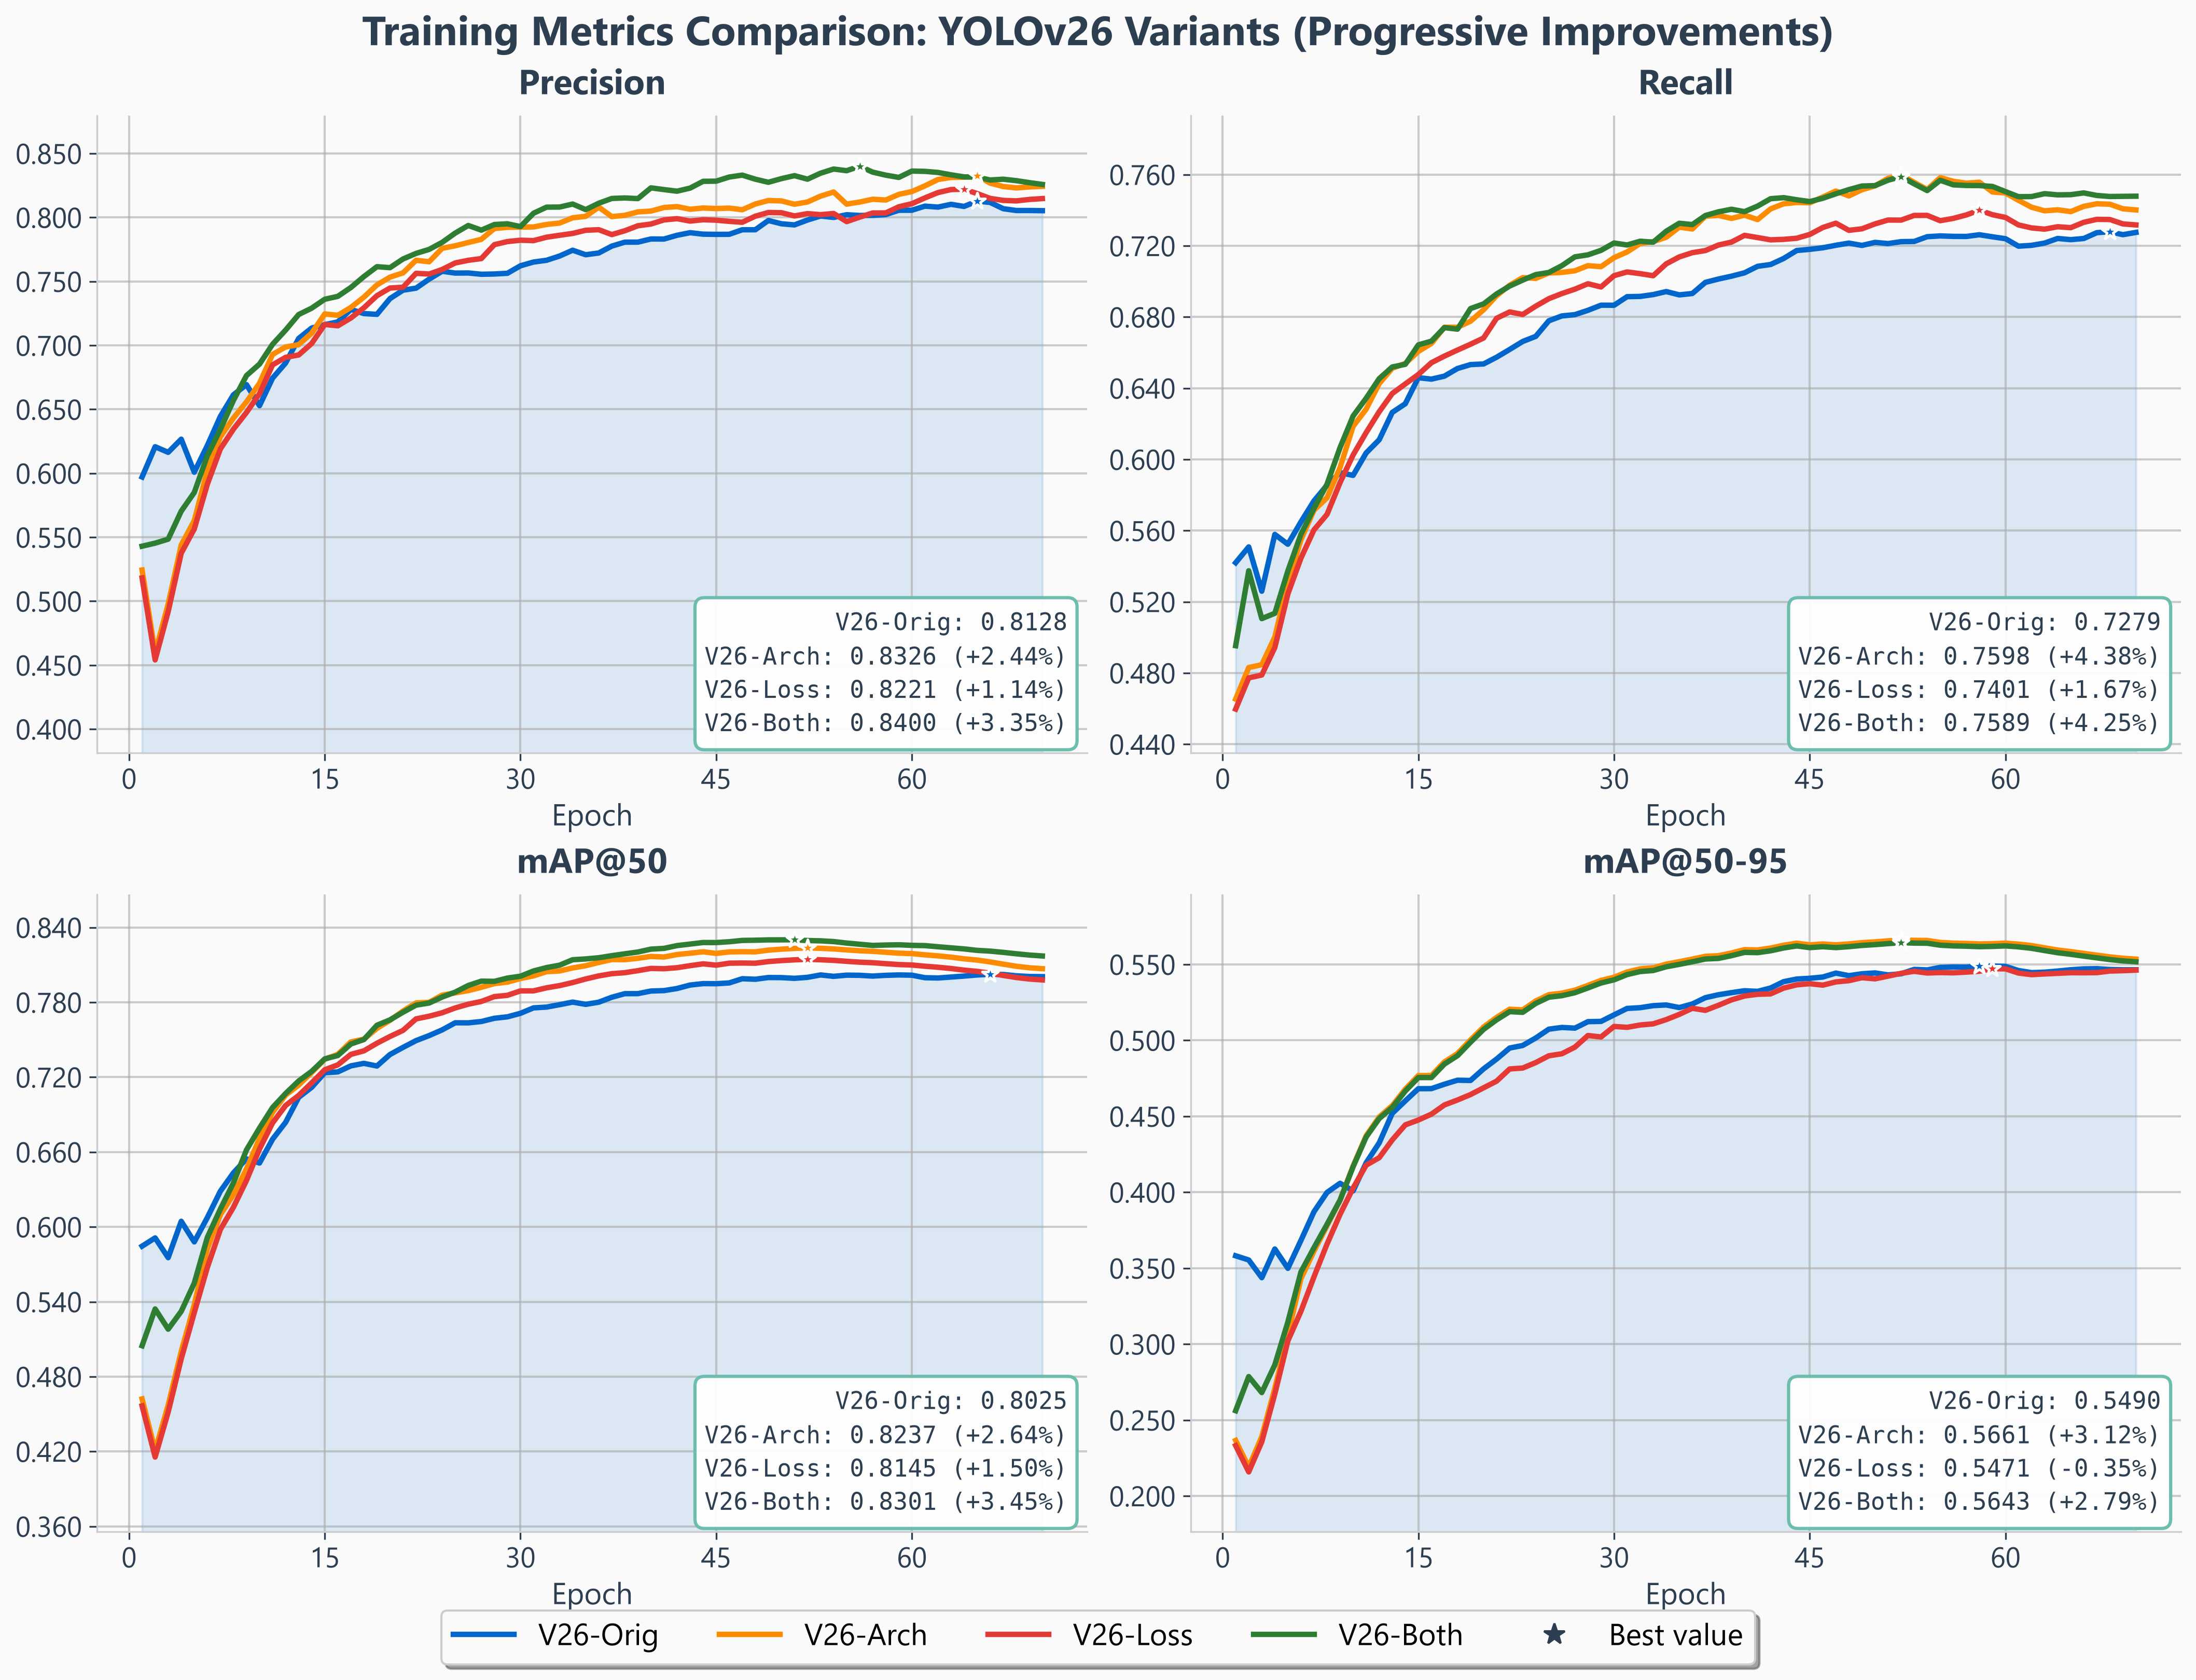
\includegraphics[width=0.98\linewidth]{TrainingGrafs/v26_metrics_4variant_compare.png}
\caption{YOLO26s training dynamics, all four configurations of
Table~\ref{tab:decomp}. Curves are per-epoch \textbf{validation} metrics; the
annotated end values are the corresponding \textbf{test} means over three seeds,
so they match Table~\ref{tab:decomp} rather than the curve maxima. The ordering
is established within the first fifteen epochs and never crosses, so the ranking
is not an artefact of where training stopped. Note the mAP$_{50\text{-}95}$
panel: the loss axis alone (red) tracks the baseline and ends slightly
\emph{below} it, which is the $-0.35\%$ of Table~\ref{tab:decomp} seen as a
trajectory.}
\label{fig:curves26}
\end{figure*}

\begin{figure*}[t]
\centering
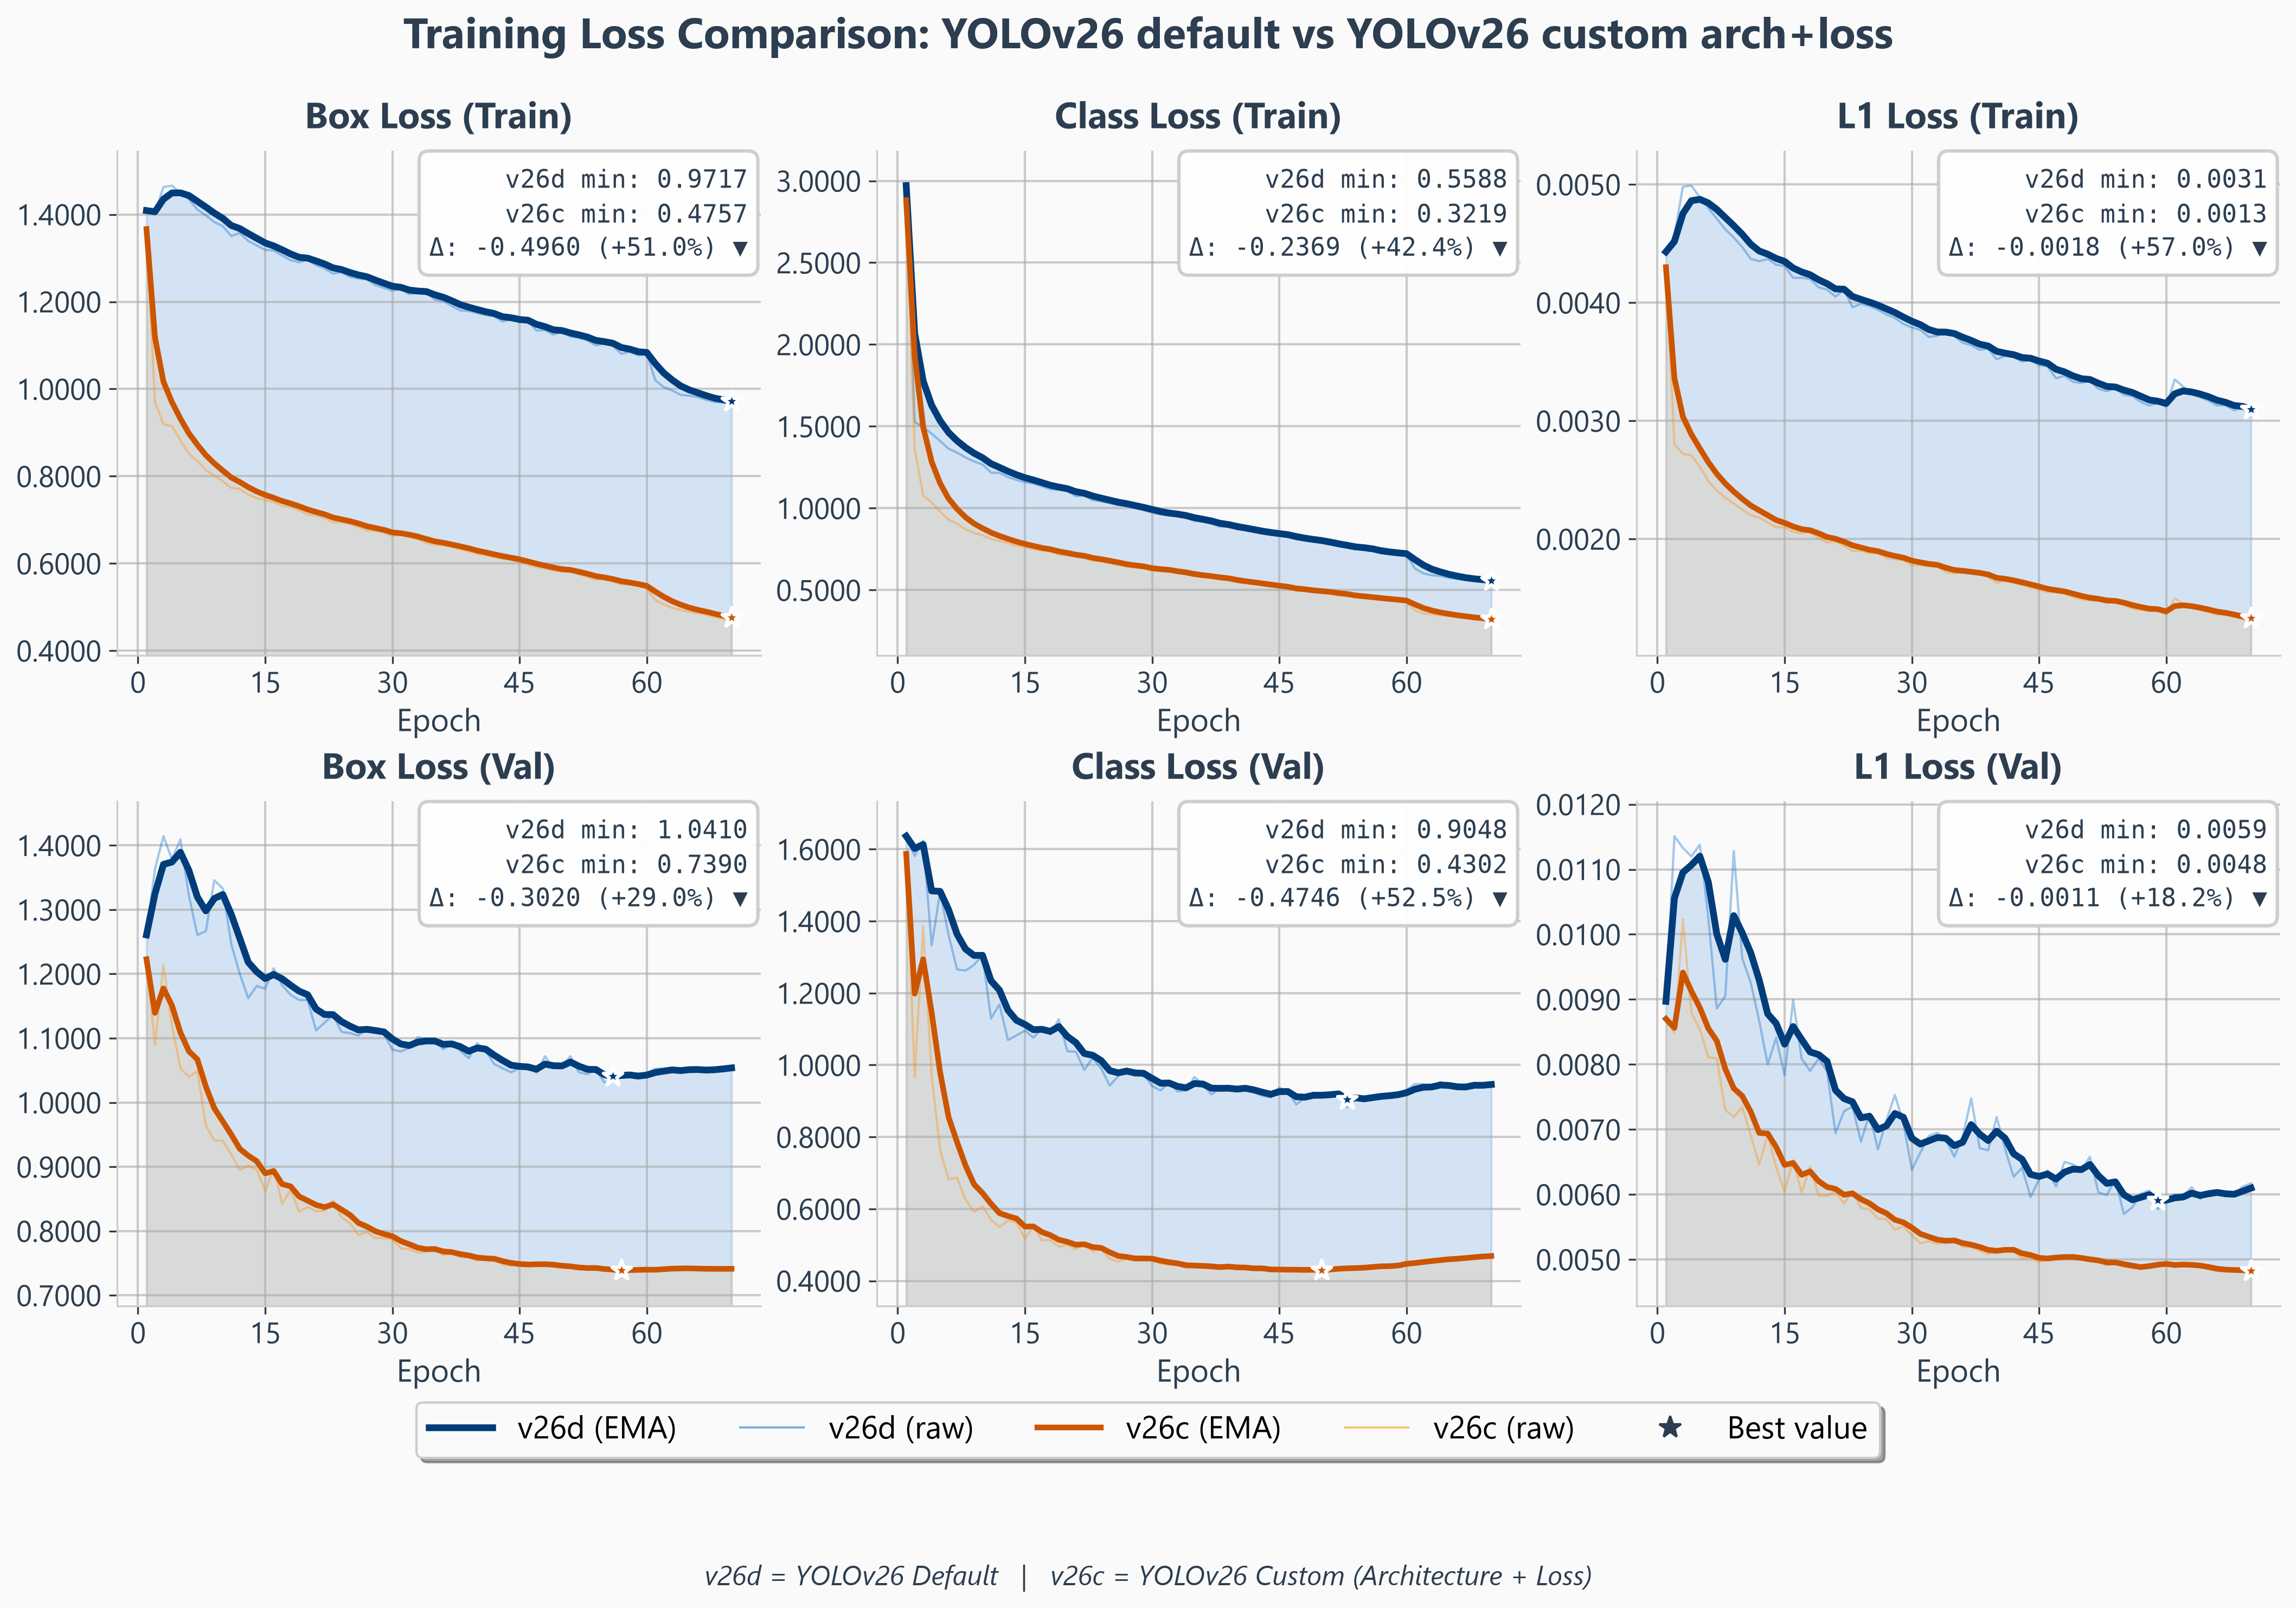
\includegraphics[width=0.98\linewidth]{TrainingGrafs/v26_metrics_loss_only.png}
\caption{YOLO26s \textbf{loss components}, baseline (\texttt{v26d}) versus the
recommended architecture$+$loss configuration (\texttt{v26c}); train on the top
row, validation on the bottom, EMA-smoothed in bold with the raw per-epoch
traces behind and the best value starred. Detection quality is not repeated
here --- the validation mAP, precision and recall curves are in
Fig.~\ref{fig:curves26}, where all four configurations can be compared at once.
All three terms fall substantially: box $-51.0\%$, classification $-42.4\%$ and
$\ell_1$ $-57.0\%$ on train, and $-29.0\%$, $-52.5\%$ and $-18.2\%$ on
validation, so the improvement is visible in the objective itself and not only
in the evaluated metrics. Both regression terms reach their validation minimum
late (box at epoch~$57$, $\ell_1$ at $60$) and stay flat to the end of the
schedule. The third panel is labelled \textbf{$\ell_1$ loss} rather than DFL:
YOLO26 sets $\mathrm{reg\_max}=1$ and substitutes an image-normalised $\ell_1$
term (Table~\ref{tab:implsdiff}), which is directly visible here and is the
structural difference Section~\ref{sec:disc:why} uses to explain why curriculum
area weighting does not transfer to this detector.}
\label{fig:loss26}
\end{figure*}

\begin{figure*}[t]
\centering
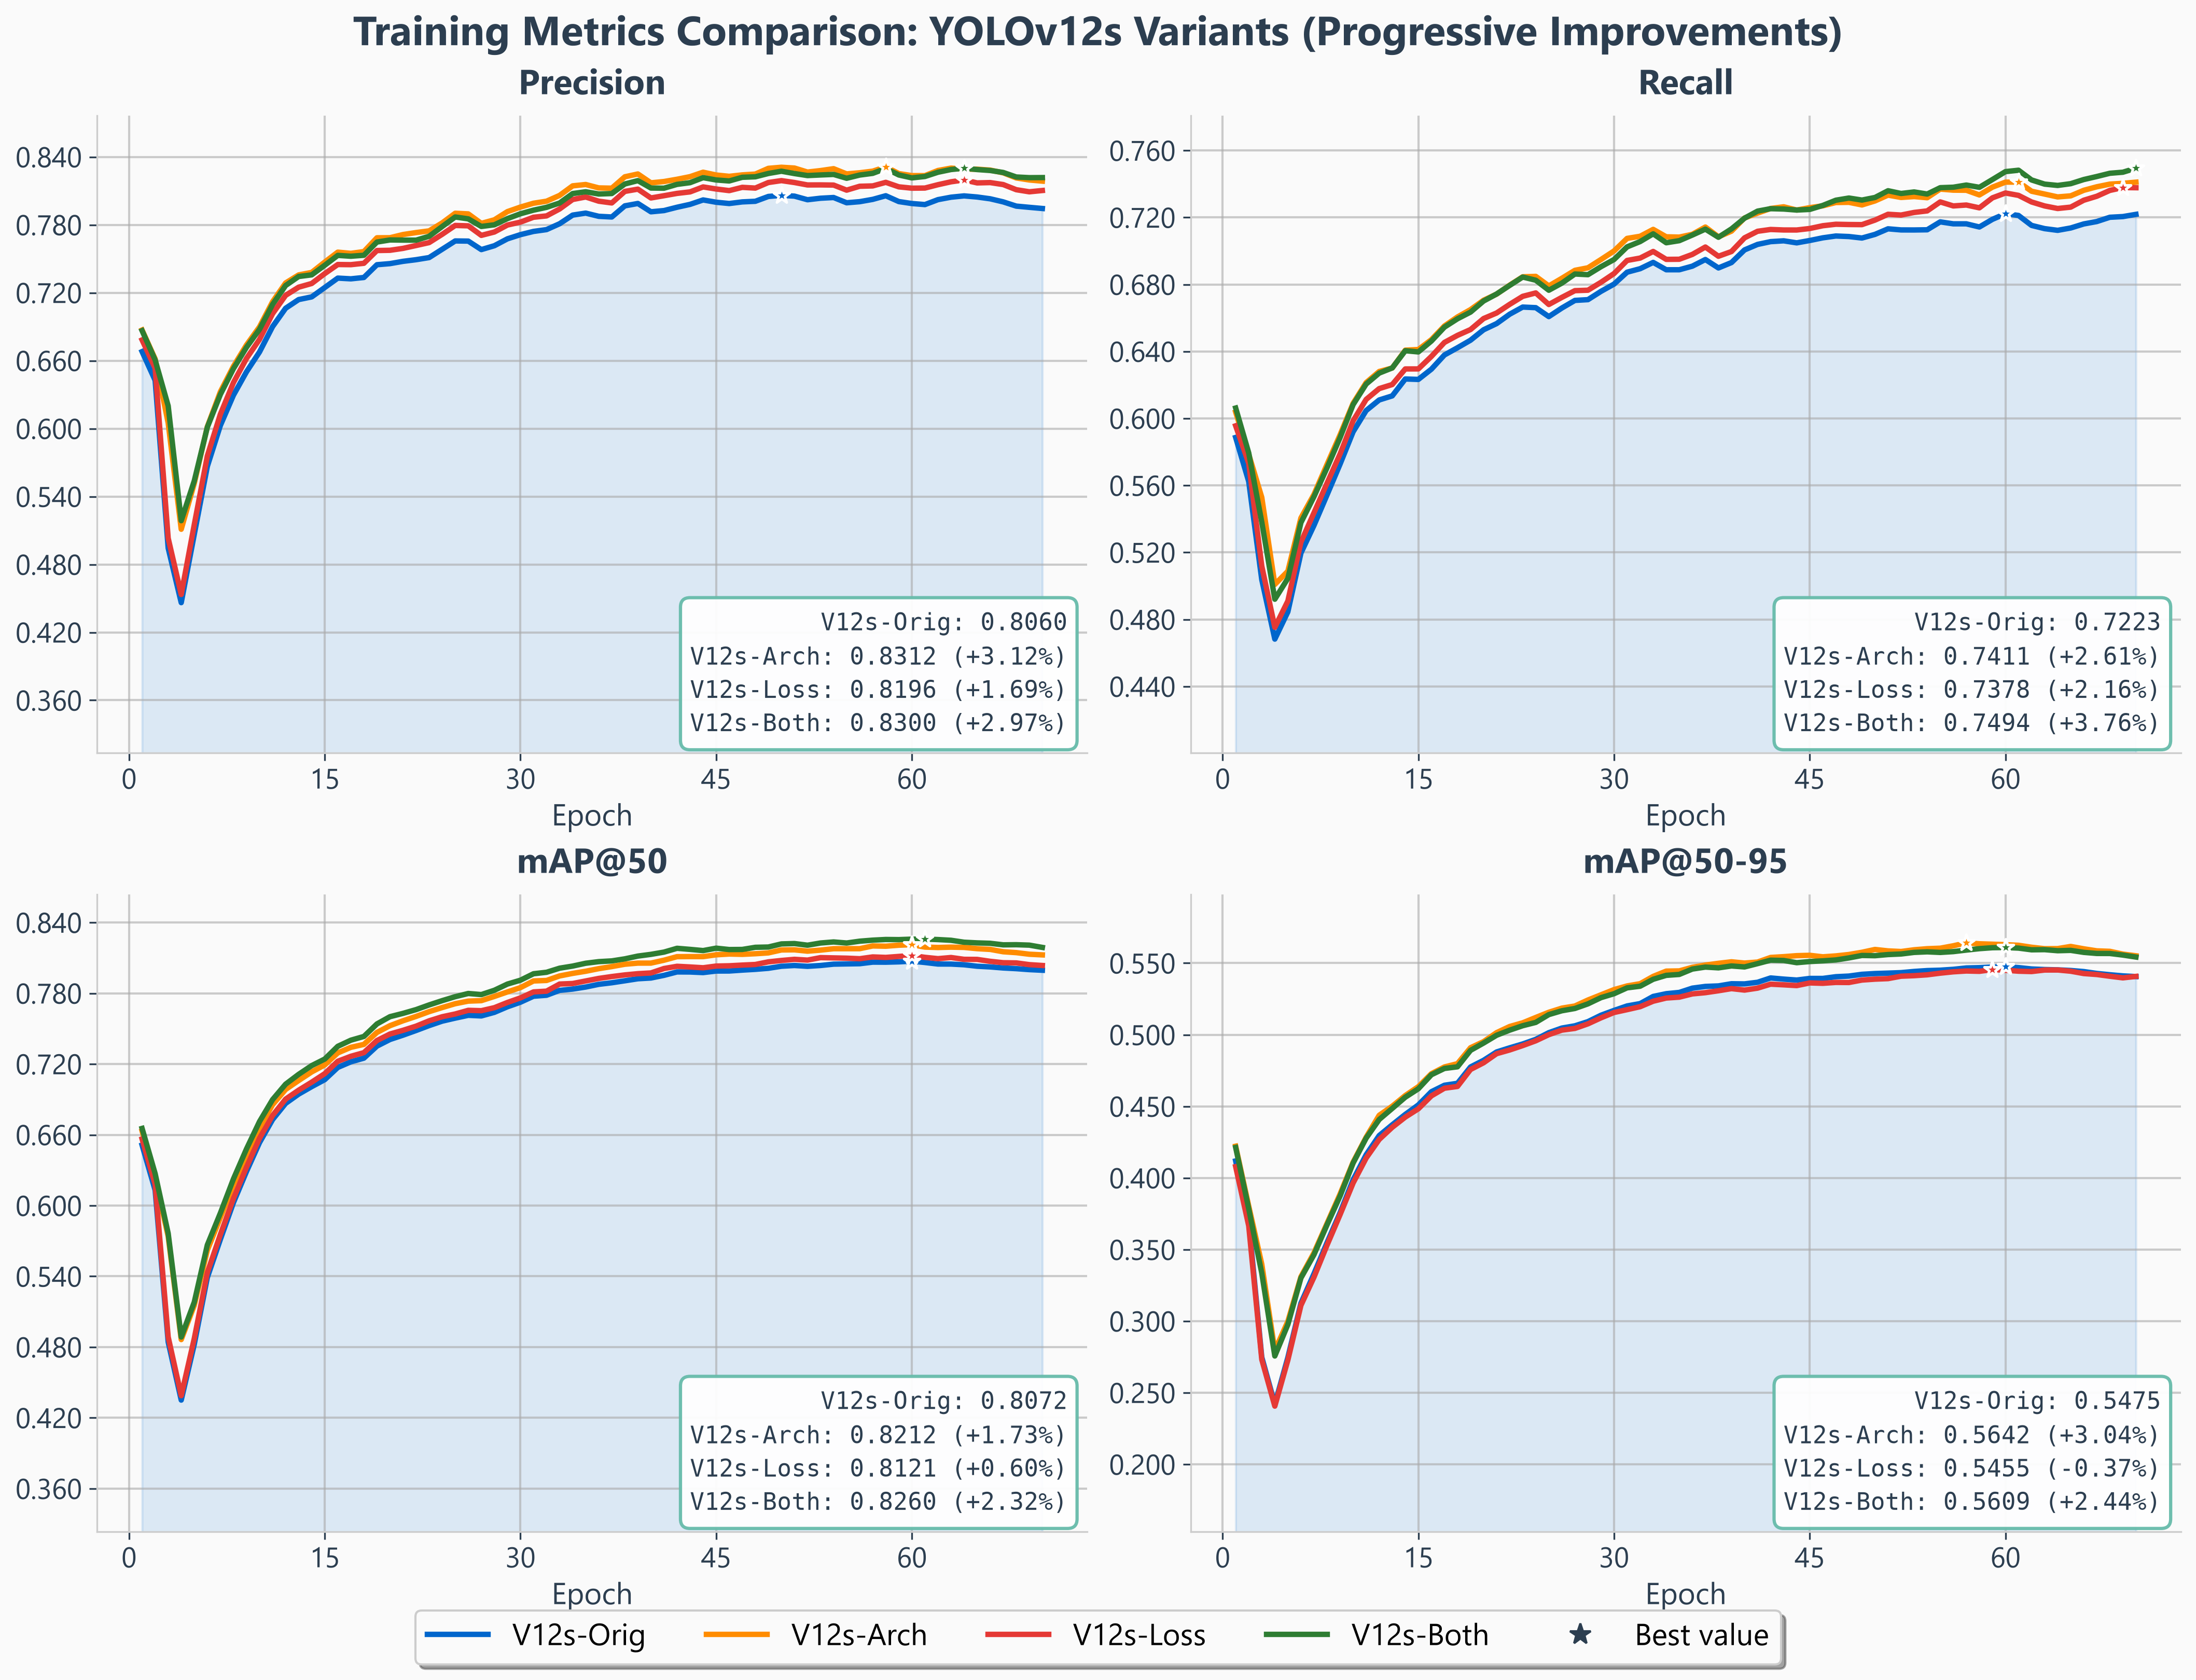
\includegraphics[width=0.98\linewidth]{TrainingGrafs/metrics_4variant_compare.png}
\caption{YOLOv12s training dynamics, same convention as
Fig.~\ref{fig:curves26}. The mAP$_{50\text{-}95}$ panel shows the same signature
as YOLO26 --- the loss axis alone ends $-0.37\%$ below the baseline while every
configuration containing the architecture ends above it --- which is the one
part of the loss mechanism's behaviour that is common to both detectors.}
\label{fig:curves12}
\end{figure*}

\begin{figure*}[t]
\centering
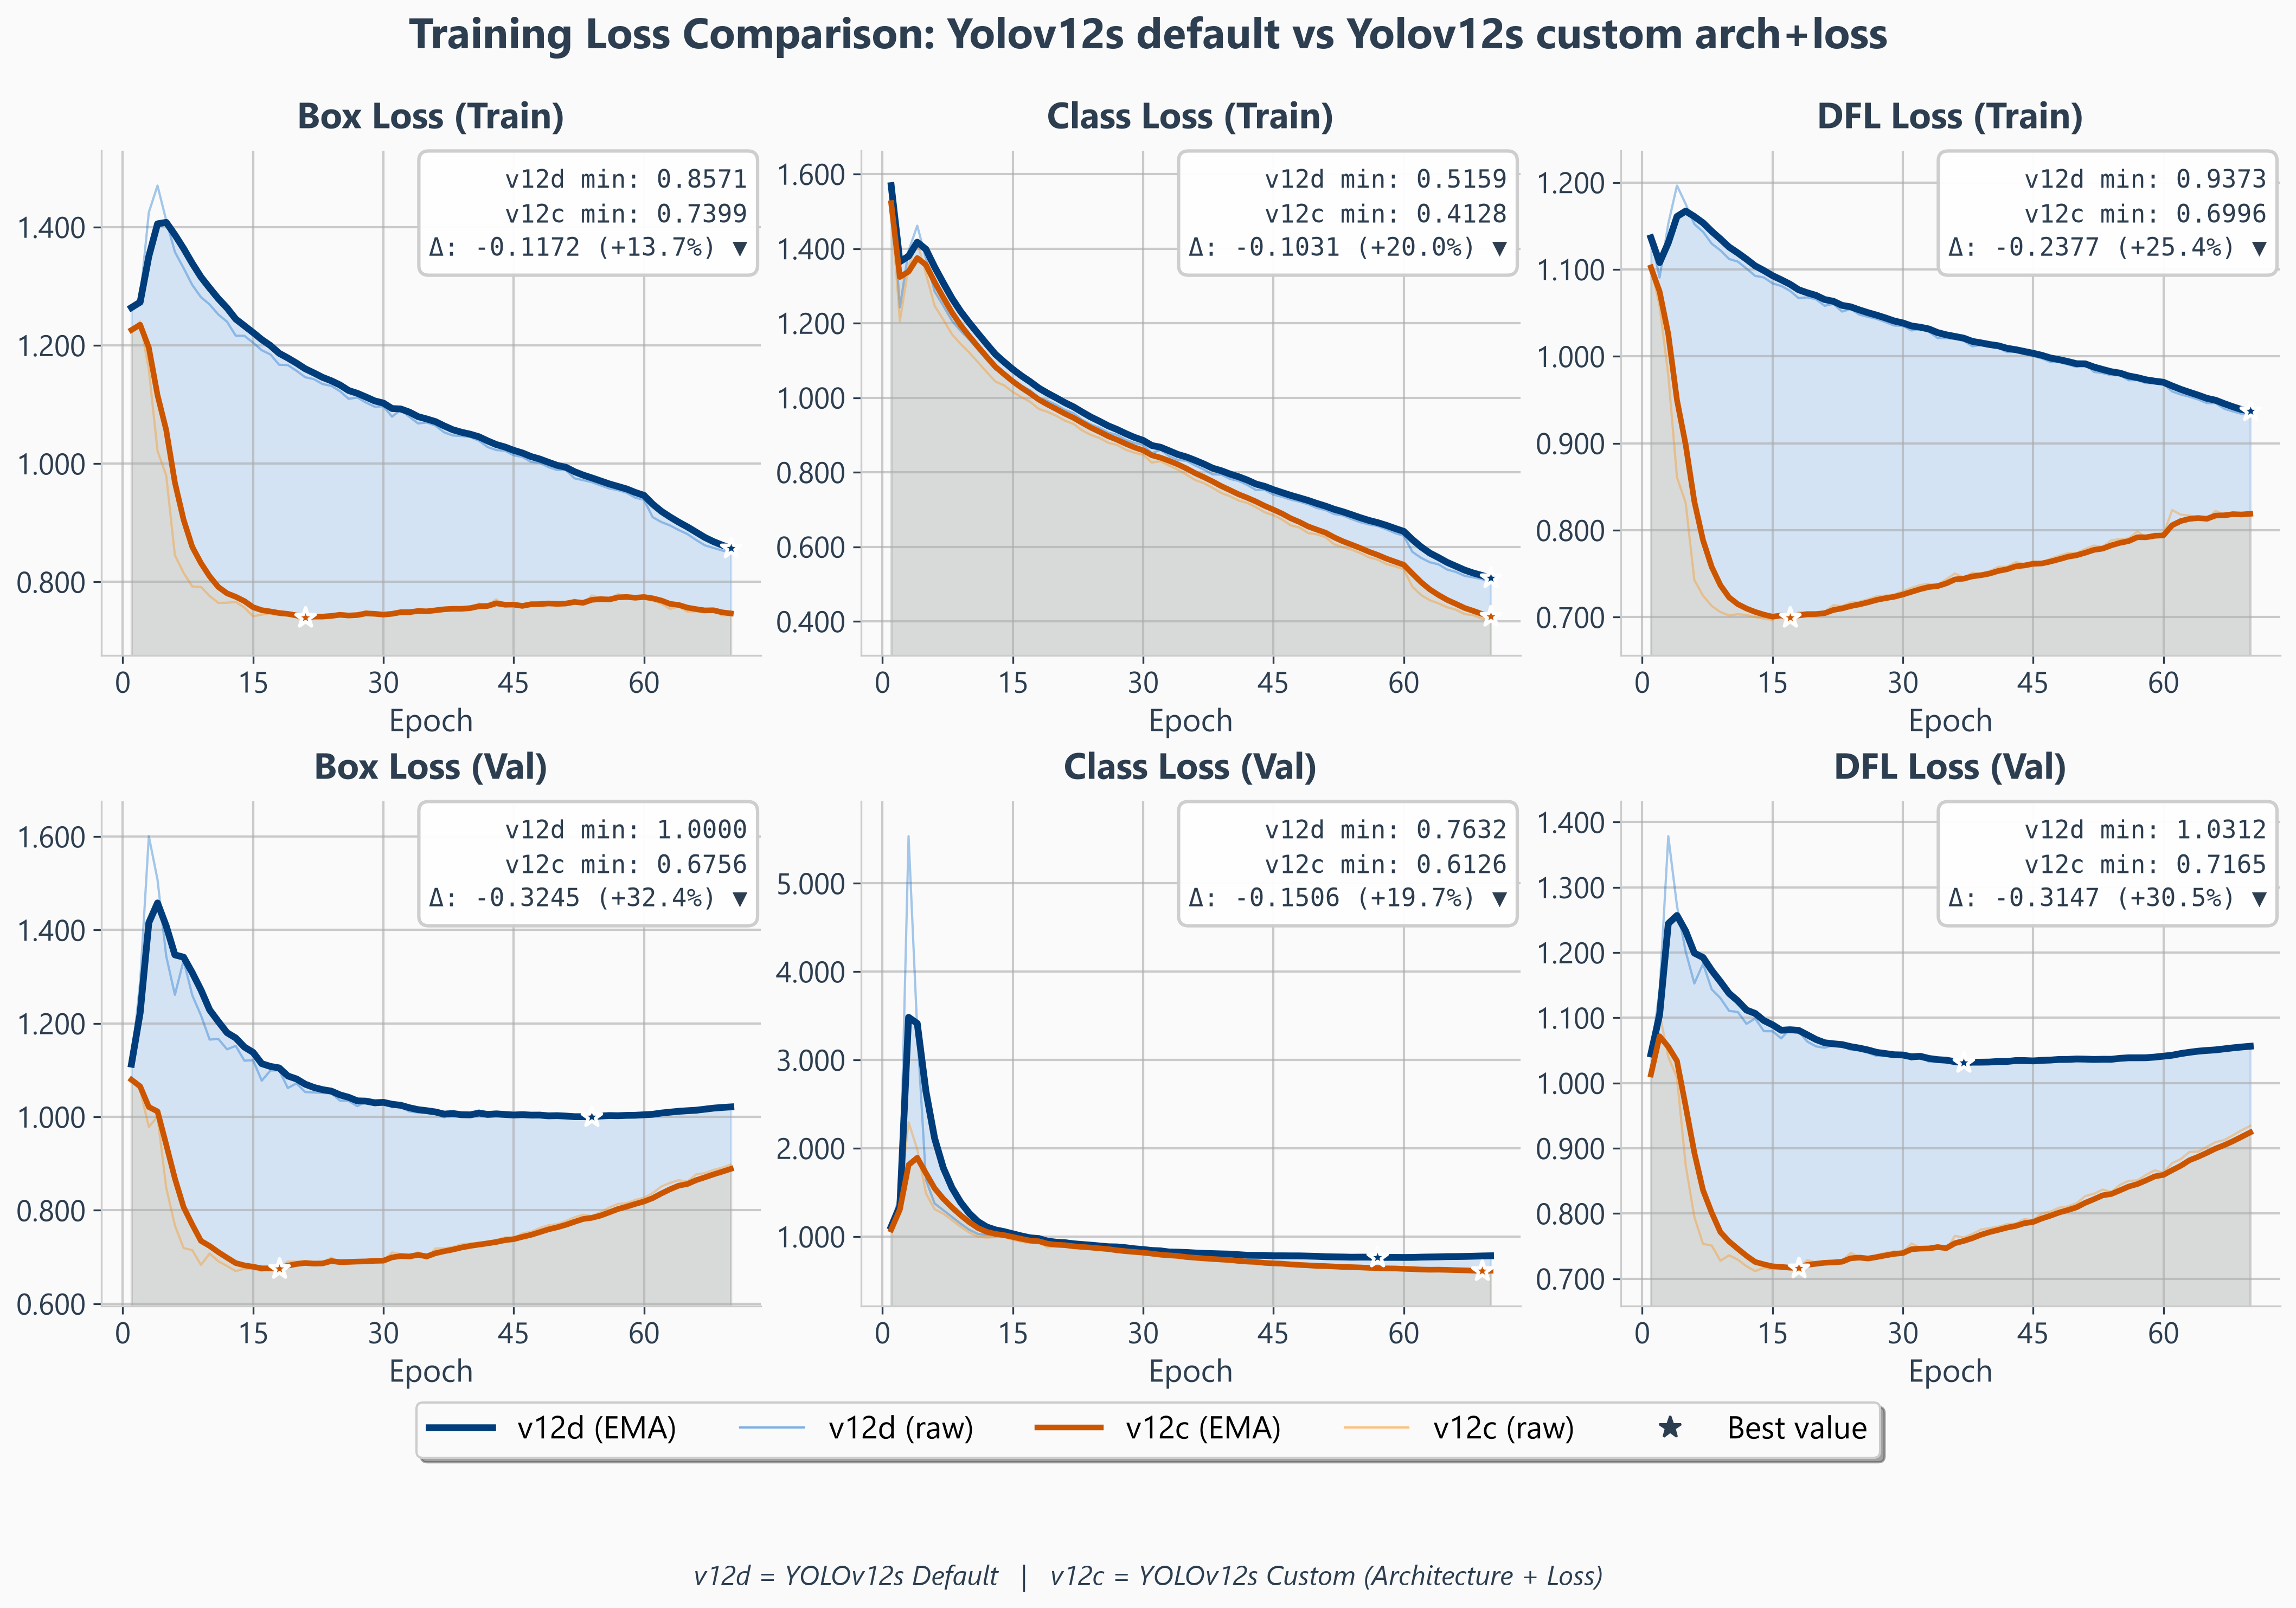
\includegraphics[width=0.98\linewidth]{TrainingGrafs/metrics_loss_only_v12.png}
\caption{YOLOv12s \textbf{loss components}, baseline (\texttt{v12d}) versus the
recommended configuration (\texttt{v12c}), same convention as
Fig.~\ref{fig:loss26}; the corresponding metric curves are in
Fig.~\ref{fig:curves12}. Box loss falls $13.7\%$ on train and $32.4\%$ on
validation, classification $20.0\%$ and $19.7\%$, DFL $25.4\%$ and $30.5\%$.
Two contrasts with Fig.~\ref{fig:loss26} matter. The third panel here is a
genuine \textbf{DFL} over $16$ bins, not an $\ell_1$ surrogate, which is the
difference Table~\ref{tab:implsdiff} records. And where YOLO26's regression
terms bottom out at the very end of the schedule, YOLOv12's reach their
validation minimum near epoch~$18$ --- box $0.676$, DFL $0.717$ --- and climb
steadily thereafter, while mAP$_{50}$ in Fig.~\ref{fig:curves12} keeps improving
to roughly epoch~$60$. The regression head overfits long before the detector
stops gaining, which is why checkpoints are selected on validation mAP rather
than on loss.}
\label{fig:loss12}
\end{figure*}


\subsubsection*{What the loss curves show}

Figures~\ref{fig:loss26} and \ref{fig:loss12} give the three loss components for
each detector, baseline against the recommended configuration, on the training
and validation splits. They carry no metric panels: mAP, precision and recall
are already in Figs.~\ref{fig:curves26} and \ref{fig:curves12}, where all four
configurations appear together rather than only two, so the loss figures are
left to show the objective alone. Every term falls on both models, and by a wide
margin on YOLO26 --- box $-51.0\%$, classification $-42.4\%$, $\ell_1$ $-57.0\%$
on the training split. Two details are worth drawing out because they bear on
the argument rather than on the headline.

\emph{The third loss term is a different objective on each detector, and the
figures say so on their axis labels.} YOLO26's panel reads $\ell_1$ loss;
YOLOv12's reads DFL loss. This is the $\mathrm{reg\_max}$ difference of
Table~\ref{tab:implsdiff} made visible, and it is the mechanism
Section~\ref{sec:disc:why} invokes to explain why curriculum area weighting ---
which leans on a distributional, anchor-relative term --- does not survive the
move to a scale-absolute $\ell_1$ surrogate.

\emph{The two detectors overfit in different terms, and on different
timescales.} On YOLO26 the two \emph{regression} terms fall for essentially the
whole schedule: validation box reaches its minimum at epoch $57$ and $\ell_1$ at
epoch $60$, both then flat, so the box head is still being paid to keep learning
when training stops. Only the classification term turns, mildly, after roughly
epoch $48$ --- and it turns in the baseline as well, so it is a property of the
schedule rather than of our modifications. On YOLOv12 the pattern is inverted
and far sharper: validation box and DFL bottom out near epoch $18$, at $0.676$
and $0.717$, and climb for the remaining fifty epochs while mAP$_{50}$ keeps
improving to roughly epoch $60$. The regression head overfits long before the
detector stops gaining. Final-epoch loss is therefore a poor stopping criterion
on YOLOv12 in particular, and the checkpoint rule used throughout --- best
validation mAP, never lowest loss --- is what keeps the two detectors
comparable despite the difference.



\subsection{Where the Gains Land, by Object Size}
\label{sec:results:persize}

\begin{table*}[t]
\centering
\caption{Per-size effect of each axis on the test split. \textbf{L} is the loss
axis alone, \textbf{A} the architecture axis alone, \textbf{A$+$L} both;
$\Delta$ is the percentage change of A$+$L over that detector's baseline. Every
cell is the mean of \textbf{three seeds}. Size buckets are the COCO \emph{area}
convention ($32^2$ / $96^2$ px$^2$), matching the evaluator. Bold marks the best
of the four columns in that row.}
\label{tab:persize}
\small
\begin{tabular}{@{}ll rrrr r@{\hspace{4mm}} rrrr r@{}}
\toprule
& & \multicolumn{5}{c}{\textbf{YOLO26s}} & \multicolumn{5}{c}{\textbf{YOLOv12s}} \\
\cmidrule(lr){3-7}\cmidrule(lr){8-12}
& Metric & Base & L & A & A$+$L & $\Delta$ & Base & L & A & A$+$L & $\Delta$ \\
\midrule
\multicolumn{12}{@{}l}{\textbf{Small} — area $<32^2$ px$^2$}\\
& mAP$_{50}$  & 77.26 & 78.61 & 79.83 & \textbf{79.91} & $+3.44$  & 77.65 & 77.93 & 78.79 & \textbf{79.87} & $+2.85$ \\
& mAP$_{50\text{-}95}$  & 50.64 & 50.50 & \textbf{52.85} & 52.82 & $+4.31$  & 49.88 & 49.66 & \textbf{51.65} & 51.60 & $+3.45$ \\
& Precision  & 77.31 & 78.25 & 80.06 & \textbf{80.97} & $+4.73$  & 76.81 & 79.08 & \textbf{81.07} & 80.06 & $+4.24$ \\
& Recall  & 72.10 & 72.59 & \textbf{74.57} & 74.20 & $+2.91$  & 70.29 & 71.16 & 71.25 & \textbf{73.67} & $+4.82$ \\
& F1  & 74.62 & 75.32 & 77.22 & \textbf{77.44} & $+3.78$  & 73.40 & 74.91 & 75.85 & \textbf{76.74} & $+4.54$ \\
\addlinespace
\multicolumn{12}{@{}l}{\textbf{Medium} — area $32^2$--$96^2$ px$^2$}\\
& mAP$_{50}$  & 86.60 & 87.26 & 87.28 & \textbf{88.59} & $+2.30$  & 87.65 & 87.54 & \textbf{87.78} & 87.42 & $-0.26$ \\
& mAP$_{50\text{-}95}$  & 65.46 & 65.38 & 66.08 & \textbf{66.16} & $+1.07$  & 65.12 & 64.46 & \textbf{65.65} & 64.49 & $-0.98$ \\
& Precision  & 91.70 & 91.01 & 90.98 & \textbf{93.02} & $+1.45$  & 88.40 & 88.78 & 91.25 & \textbf{92.35} & $+4.46$ \\
& Recall  & 79.04 & 80.38 & \textbf{82.90} & 82.23 & $+4.03$  & 80.77 & \textbf{81.76} & 81.30 & 79.08 & $-2.09$ \\
& F1  & 84.90 & 85.36 & 86.75 & \textbf{87.29} & $+2.82$  & 84.41 & 85.13 & \textbf{85.99} & 85.20 & $+0.93$ \\
\addlinespace
\multicolumn{12}{@{}l}{\textbf{Large} — area $>96^2$ px$^2$}\\
& mAP$_{50}$  & 81.82 & 81.85 & \textbf{83.26} & 80.83 & $-1.21$  & 82.93 & 82.63 & \textbf{84.68} & 82.79 & $-0.17$ \\
& mAP$_{50\text{-}95}$  & 60.54 & 59.87 & \textbf{60.84} & 59.49 & $-1.73$  & 57.62 & 58.67 & \textbf{60.52} & 59.90 & $+3.94$ \\
& Precision  & 79.98 & 77.29 & \textbf{87.59} & 77.88 & $-2.62$  & 83.97 & 83.94 & \textbf{87.95} & 83.43 & $-0.64$ \\
& Recall  & 76.37 & \textbf{82.49} & 80.71 & 80.20 & $+5.01$  & 74.78 & \textbf{79.65} & 78.21 & 77.92 & $+4.20$ \\
& F1  & 78.13 & 79.81 & \textbf{84.01} & 79.02 & $+1.14$  & 79.11 & 81.74 & \textbf{82.80} & 80.58 & $+1.86$ \\
\bottomrule
\end{tabular}
\end{table*}


Table~\ref{tab:persize} resolves each axis by object size, which is where the
two detectors stop resembling each other. Three patterns are worth naming.

\emph{The gains are concentrated on small objects and are paid for elsewhere.}
On both detectors the combined configuration improves small-object mAP$_{50}$
(YOLO26 $+3.44\%$, YOLOv12 $+2.85\%$) and small-object F1 ($+3.78\%$ and
$+4.54\%$), while medium objects are flat to negative and mAP$_{50\text{-}95}$
falls at every size except small. Since small and medium together account for
$75.0\%$ of instances (Table~\ref{tab:sizes}), that is the
right trade to make --- but the headline number is
not a uniform improvement and should not be reported as one.

\emph{The two detectors buy the same small-object gain with opposite
currencies.} On YOLO26 the improvement comes from precision ($+5.07\%$) with
recall moving less ($+2.91\%$); on YOLOv12 precision and recall rise together
($+4.24\%$ and $+4.82\%$). Both detectors reach a similar small-object F1 gain
($+3.78\%$ and $+4.54\%$), but YOLO26 gets there by becoming more selective and
YOLOv12 by finding more --- the per-size trace of the one-to-one versus
NMS-based assignment difference discussed in Section~\ref{sec:disc:why}.

\emph{The large-object cost belongs to the combination, not to the
architecture.} Taken alone, the architecture axis leaves large-object
mAP$_{50\text{-}95}$ intact on YOLO26 ($+0.51\%$) and improves it markedly on
YOLOv12 ($+5.03\%$), so deleting the stride-32 \emph{detection} branch does not
by itself degrade large objects --- the retained stride-32 backbone still
supplies the context they need. What costs large objects is adding the loss axis
on top: from the architecture cell to the combination, YOLO26 gives up $2.43$
points of large-object mAP$_{50}$ and YOLOv12 $1.89$, both beyond
$2\,\mathrm{SE}$. The mechanism that sharpens small-object detection is the one
that blunts large-object localisation, on both detectors.

\subsubsection*{Why these are fixed configurations rather than per-cell maxima}

Each column of Table~\ref{tab:persize} is a single configuration evaluated at
all three sizes. It is not the best run per cell, and for most cells it is not
the campaign maximum: on large-object mAP$_{50}$, for instance, some run in the
YOLO26 campaign reaches $85.55$ against our configuration's $80.35$. We report
the fixed configuration deliberately, for two reasons.

First, a per-cell maximum describes a model that does not exist. One cannot
deploy the configuration that happens to lead on large objects together with the
one that leads on small objects; a table assembled that way would report an
unattainable system.

Second, and more importantly, those maxima are largely noise. Selecting the
maximum of $N$ draws from a distribution with standard deviation $\sigma$ yields,
from sampling alone, an expected excess of approximately
$\sigma\sqrt{2\ln N}$ above the mean. With $N=174$ YOLO26 runs and the measured
$\sigma = 2.258$ on mAP$_{50}^{\text{large}}$ --- the noisiest metric in the
study --- that is $7.25$ points. The $5.20$-point gap between our configuration
and the campaign maximum is therefore \emph{smaller} than what pure noise would
be expected to produce, and the corresponding maximum is a single unrepeated
draw. The same calculation on mAP$_{50}^{\text{small}}$, where
$\sigma = 0.428$, gives an expected noise maximum of $1.37$ points against an
observed gap of $0.32$. Reporting per-cell maxima would amount to tabulating the
selection bias we measured in Section~\ref{sec:method:protocol}.

\subsection{Per-Class Behaviour}
\label{sec:results:perclass}

\begin{table*}[t]
\centering
\caption{Per-class, per-size performance on the test split: baseline versus the
recommended configuration, both models, means of three seeds. Size buckets are
the COCO area convention. \texttt{bag} is the weakest class at every size on
both detectors and the ordering \texttt{trolley} $>$ \texttt{backpack} $>$
\texttt{bag} holds in all eighteen cells.}
\label{tab:perclasssize}
\small
\begin{tabular}{@{}ll rrr rrr@{}}
\toprule
& & \multicolumn{3}{c}{AP$_{50}$} & \multicolumn{3}{c}{AP$_{50\text{-}95}$} \\
\cmidrule(lr){3-5}\cmidrule(lr){6-8}
Class & Size & Base & A$+$L & $\Delta$ & Base & A$+$L & $\Delta$ \\
\midrule
\multicolumn{8}{@{}l}{\textbf{YOLO26s} \; --- \; p2dys-p234rich $+$ $\beta{=}1$}\\
\textit{backpack} & small & 78.82 & 81.10 & $+2.28$ & 51.11 & 53.91 & $+2.79$ \\
 & medium & 89.69 & 91.99 & $+2.30$ & 67.88 & 69.75 & $+1.87$ \\
 & large & 82.93 & 86.53 & $+3.60$ & 56.49 & 58.56 & $+2.06$ \\
\textit{bag} & small & 67.78 & 70.46 & $+2.68$ & 42.78 & 44.60 & $+1.82$ \\
 & medium & 76.85 & 79.64 & $+2.79$ & 54.88 & 55.77 & $+0.90$ \\
 & large & 85.74 & 85.50 & $-0.25$ & 68.87 & 66.36 & $-2.51$ \\
\textit{trolley} & small & 85.47 & 88.86 & $+3.39$ & 58.09 & 60.24 & $+2.15$ \\
 & medium & 93.16 & 93.99 & $+0.84$ & 73.98 & 72.83 & $-1.14$ \\
 & large & 76.77 & 70.48 & $-6.29$ & 56.00 & 58.26 & $+2.26$ \\
\midrule
\multicolumn{8}{@{}l}{\textbf{YOLOv12s} \; --- \; \texttt{ls\_shift} $+$ curriculum weighting}\\
\textit{backpack} & small & 77.71 & 80.48 & $+2.76$ & 50.49 & 52.87 & $+2.38$ \\
 & medium & 90.99 & 92.53 & $+1.54$ & 66.99 & 68.65 & $+1.66$ \\
 & large & 85.28 & 82.09 & $-3.18$ & 58.70 & 57.92 & $-0.78$ \\
\textit{bag} & small & 67.45 & 70.83 & $+3.37$ & 41.75 & 43.36 & $+1.61$ \\
 & medium & 77.30 & 75.79 & $-1.51$ & 54.72 & 53.19 & $-1.53$ \\
 & large & 81.33 & 86.58 & $+5.25$ & 66.41 & 66.79 & $+0.38$ \\
\textit{trolley} & small & 87.64 & 88.22 & $+0.58$ & 57.68 & 58.74 & $+1.06$ \\
 & medium & 94.88 & 94.07 & $-0.81$ & 73.58 & 72.10 & $-1.48$ \\
 & large & 81.93 & 79.67 & $-2.26$ & 48.08 & 55.16 & $+7.08$ \\
\bottomrule
\end{tabular}
\end{table*}

% =====================================================================
% Size-resolved confusion matrices, baseline vs recommended, both models.
% Generated by Confusion_original_improved/make_cm_figs.py from cm_values.json.
% =====================================================================
\begin{figure*}[t]
\centering
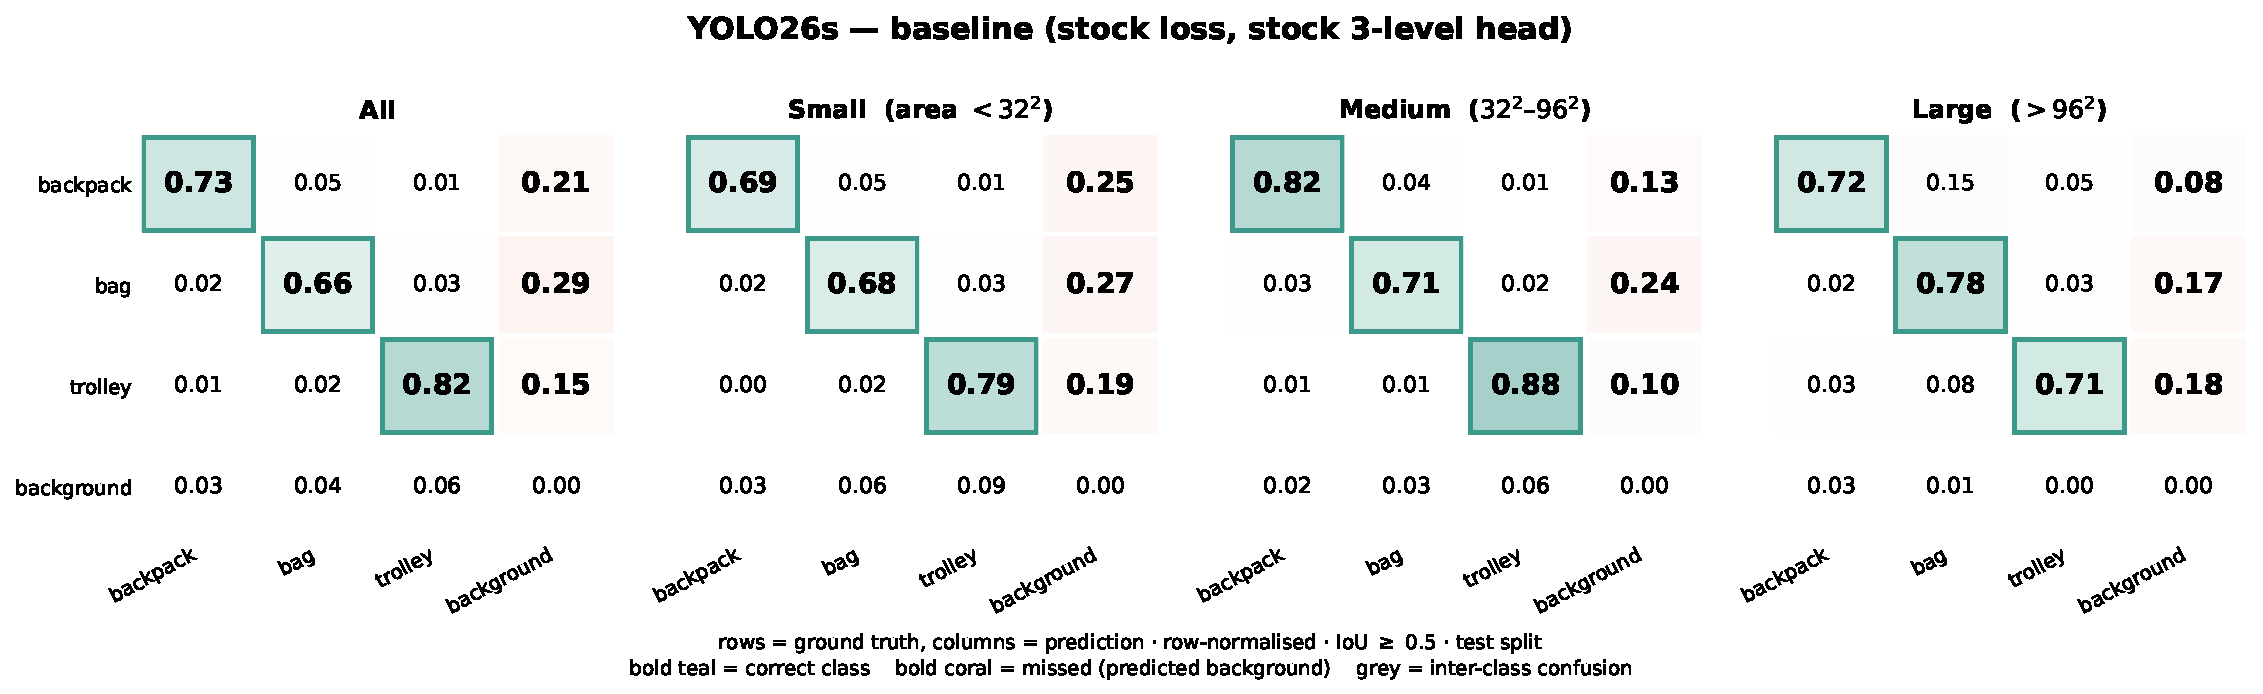
\includegraphics[width=\linewidth]{Confusion_original_improved/v26_default_cm.pdf}\\[5pt]
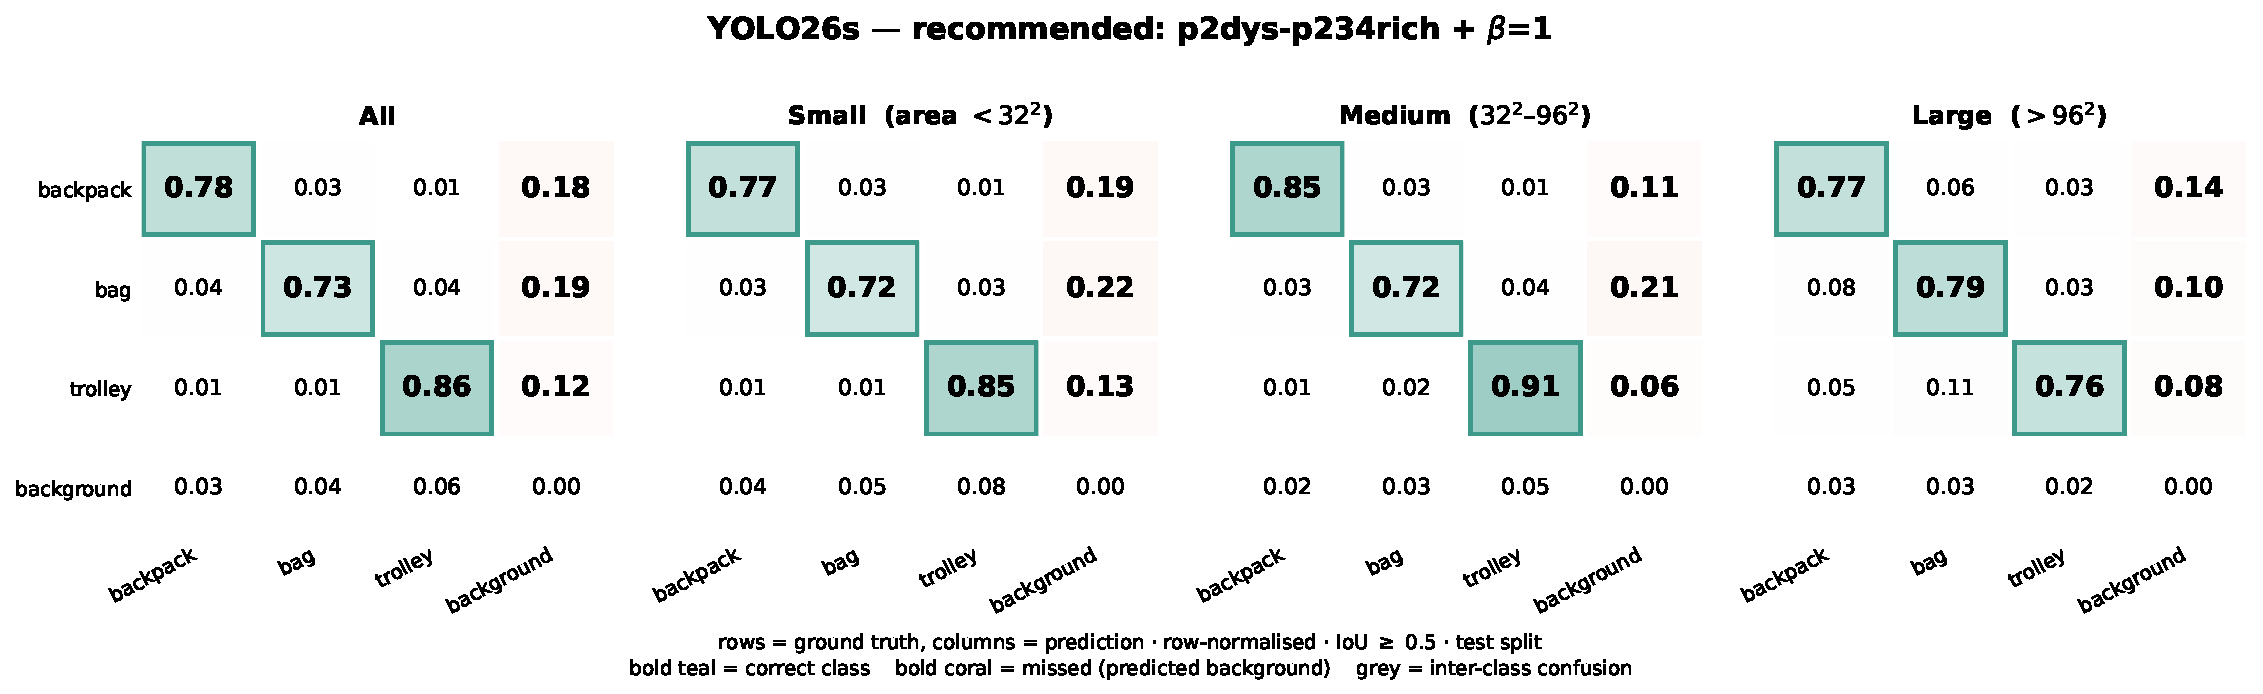
\includegraphics[width=\linewidth]{Confusion_original_improved/v26_custom_cm.pdf}
\caption{YOLO26s confusion, resolved by object size: baseline (top) and the
recommended configuration (bottom). Rows are ground truth, columns are
prediction, each row normalised, IoU $\geq 0.5$, test split. The bold teal
diagonal is the correct-class rate and the bold coral column is the \emph{miss}
rate --- ground truth predicted as background --- which for an alarm system is
the operative failure. Every class improves at every size; the largest single
change is \texttt{bag} missed to background, $0.29 \rightarrow 0.19$ overall and
$0.27 \rightarrow 0.22$ on small objects.}
\label{fig:cm26}
\end{figure*}

\begin{figure*}[t]
\centering
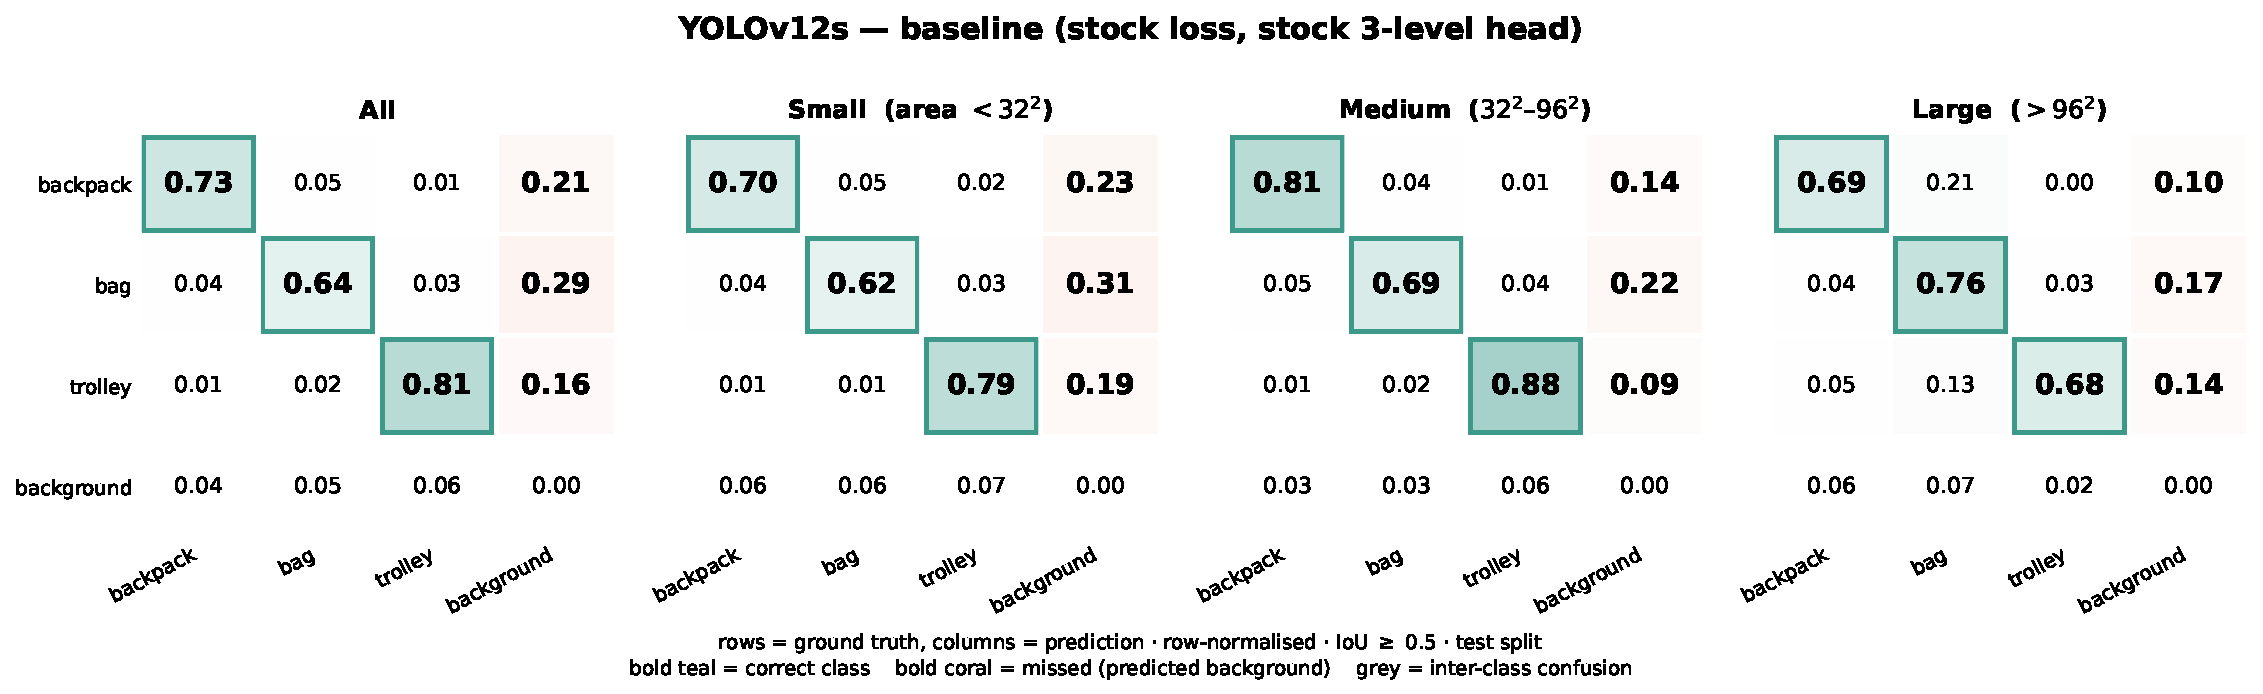
\includegraphics[width=\linewidth]{Confusion_original_improved/v12_default_cm.pdf}\\[5pt]
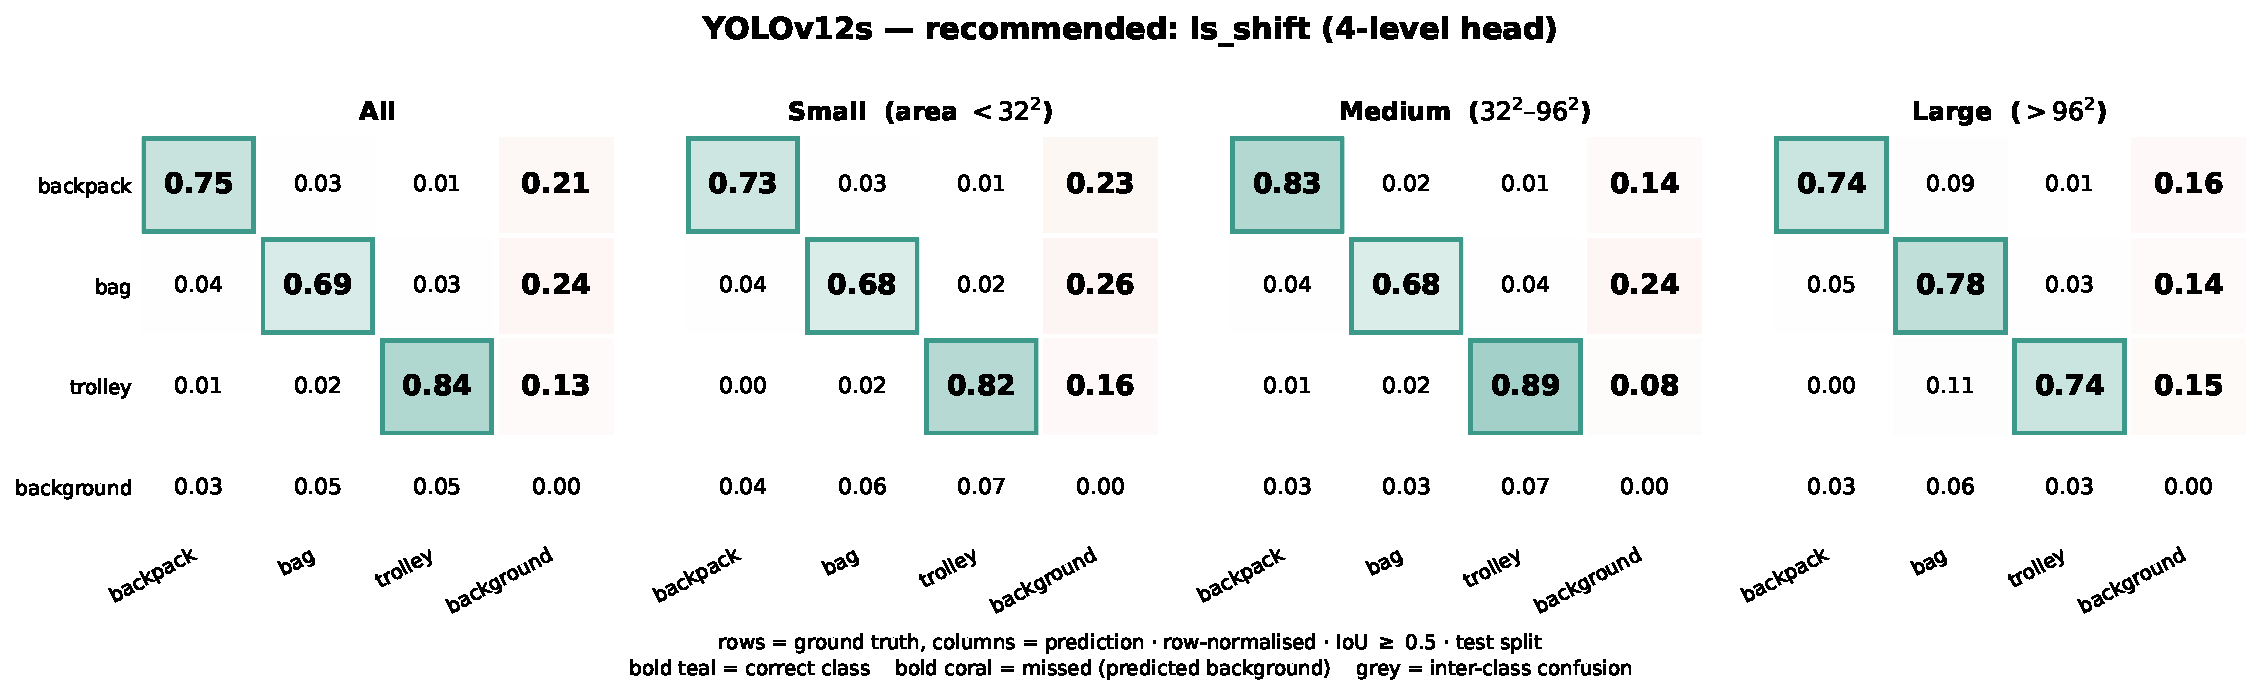
\includegraphics[width=\linewidth]{Confusion_original_improved/v12_custom_cm.pdf}
\caption{YOLOv12s confusion, same convention as Fig.~\ref{fig:cm26}: baseline
(top), recommended configuration (bottom). The pattern matches YOLO26 --- every
class improves at every size and \texttt{bag} improves most ($0.64 \rightarrow
0.69$ correct overall, misses $0.29 \rightarrow 0.24$) --- but from a lower
starting point on that class, and the residual \texttt{bag} miss rate stays
above YOLO26's.}
\label{fig:cm12}
\end{figure*}


Table~\ref{tab:perclasssize} resolves the same comparison by class as well as
size. The dominant pattern is that \textbf{\emph{bag} is the hard class at every
size and on both detectors}, and by a wide margin: at AP$_{50}$ its small-object
score is $68.4$ on YOLO26 and $66.8$ on YOLOv12, against $85.7$ and $86.5$ for
\emph{trolley} --- a gap of roughly $18$ points that neither axis closes. The
ordering \emph{trolley} $>$ \emph{backpack} $>$ \emph{bag} holds in all
eighteen class$\times$size cells.

This is consistent with the assignment diagnostics, which found per-class
behaviour essentially uniform at strides $8$ and $16$: the bag deficit is not a
matter of candidate supply, and it is therefore not something a stride-4 level
or an assignment exponent can repair. It is a classification problem --- bags
are visually heterogeneous and the class is the one most often confused with
background in the baseline confusion matrix. Both recommended configurations do
improve it slightly at AP$_{50}$ ($+0.98$ and $+1.76$ on small objects), but
neither changes its rank.

The per-class view also localises the large-object cost reported in
Section~\ref{sec:results:persize}. On YOLO26 the AP$_{50\text{-}95}$ loss at
large sizes is concentrated almost entirely in one class --- \emph{bag},
$68.36 \rightarrow 60.84$ --- while \emph{backpack} loses $2.09$ and
\emph{trolley} $1.37$. The stride-32 deletion does not degrade large objects
uniformly; it degrades the class whose large instances are least distinctive.

\subsection{What Each Axis Actually Buys}

The two axes do not improve the same things, and with three seeds the split is
clean and identical on both detectors:

\begin{center}\small
\begin{tabular}{@{}llrrrr@{}}
\toprule
& axis & P & R & mAP$_{50\text{-}95}$ & AR$_{50\text{-}95}^{\text{small}}$ \\
\midrule
\multirow{2}{*}{YOLO26s}  & Loss & $+1.14$ & $+1.67$ & $\mathbf{-0.35}$ & $-1.46$ \\
                          & Arch & $+2.44$ & $+4.38$ & $\mathbf{+3.12}$ & $-1.25$ \\
\addlinespace
\multirow{2}{*}{YOLOv12s} & Loss & $+1.69$ & $+2.16$ & $\mathbf{-0.37}$ & $-2.11$ \\
                          & Arch & $+3.12$ & $+2.61$ & $\mathbf{+3.04}$ & $+2.48$ \\
\bottomrule
\end{tabular}
\end{center}

\noindent (percentage change over each detector's own baseline). Both axes raise
precision and recall on both models. The separation is on
\textbf{mAP$_{50\text{-}95}$}: the loss axis \emph{costs} it --- $-0.35\%$ and
$-0.37\%$, two independent detectors agreeing to within $0.02$ points --- while
the architecture axis gains it, $+3.12\%$ and $+3.04\%$, agreeing to within
$0.08$. That two mechanisms reproduce their signature this closely across
detectors that share almost no implementation is the strongest regularity in the
study.

The reading is the one Section~\ref{sec:method:loss} predicts. Flattening the
alignment exponent, or re-weighting positives by scale, changes \emph{which}
detections are made and how confidently, but neither improves where a box is
placed; at stricter IoU thresholds that shows up as a small loss. Adding a
stride-4 level changes the resolution at which a small object is represented,
which improves placement directly.

The small-object recall ceiling tells a similar story. The loss axis lowers it
on both detectors ($-1.46\%$, $-2.11\%$): sharpening or re-weighting assignment
discards candidates. The architecture axis lowers it slightly on YOLO26
($-1.25\%$) but \emph{raises} it on YOLOv12 ($+2.48\%$), the one place the two
detectors disagree --- and the one where YOLOv12 keeps its stride-32 head while
YOLO26 deletes it.

\subsection{The Axes Are Substantially Redundant}
\label{sec:results:redundant}

Writing the effect of each axis alone as $\Delta_A$ and $\Delta_L$ and the
combined effect as $\Delta_{AL}$, the interaction is
$\iota = \Delta_{AL} - (\Delta_A + \Delta_L)$. On YOLO26,
$\Delta_A = +1.10$, $\Delta_L = +1.32$, $\Delta_{AL} = +1.85$ points, so
$\iota = -1.26$: the combination delivers $68\%$ of the sum of its parts. The
same computation on YOLOv12's native combinations gives $46$--$81\%$. Measured
against the architecture alone, adding a loss mechanism on YOLOv12 yields
$+0.39$, $-0.09$ and $-0.22$ points of small-object mAP$_{50}$ for curriculum
weighting, WIoU and level-balanced assignment respectively --- that is, no
reliable gain at all. The two axes compete for the same errors.

\subsection{Neither Detector's Mechanisms Transfer to the Other}
\label{sec:results:transfer}

We tested transfer in both directions and on both axes, always on the same
dataset and at matched batch size. Table~\ref{tab:transfer} gives all four cells.

\begin{table}[t]
\centering
\caption{The transfer design. Each mechanism is evaluated on the detector it was
developed for and on the other one. $\Delta$ is percentage change in
mAP$_{50}^{\text{small}}$ over that detector's own baseline; the run-to-run
standard error is $0.28$ points on YOLO26 and $0.20$ on YOLOv12, so
$|\Delta| < 0.7\%$ is not resolvable.}
\label{tab:transfer}
\small
\begin{tabular}{@{}llrr@{}}
\toprule
Axis & Mechanism & own & other \\
\midrule
Loss & curriculum weighting \; (v12) & $+0.36$ & \textit{null} \\
Loss & alignment exponent $\beta{=}1$ \; (v26) & $+1.75$ & \textit{$+0.32$} \\
Arch & level-specific blocks \; (v12) & $+1.47$ & \textit{$+0.66$} \\
Arch & drop stride 32 $+$ depth 4 \; (v26) & $+3.33$ & \textit{$+0.56$} \\
\bottomrule
\end{tabular}
\end{table}

The result is uniform: \textbf{every one of the four cross-model transfers is a
null on the primary metric.} The resolvability threshold is $0.7\%$ of the
baseline; no ``other'' cell reaches it, while three of the four ``own'' cells
clear it by a factor of at least two. This is not a case of mechanisms that help a
little less on the other detector; it is four mechanisms that stop working.

Two of them additionally do damage that the small-object metric hides. The
YOLO26 level reallocation costs YOLOv12 $6.1$ points of large-object
mAP$_{50}$ and $9.6$ at strict IoU, and $\beta=1$ costs YOLOv12 $0.9$ points of
mAP$_{50\text{-}95}$ and $2.6$ of the small-object recall ceiling. Taken across
all metrics rather than one, the YOLO26 configuration loses $20$ of $24$
matched-batch comparisons against YOLOv12's native configurations. The
YOLOv12 global-context block, evaluated on YOLO26 in two placements, scored
$+0.51$ and $+0.01$ --- in both cases \emph{below} the shared P2$+$DySample
change it was added to, so it did not merely fail to help, it displaced
something that did.

The four comparisons the YOLO26 configuration does win are exactly those its
mechanism predicts --- large-object AP for the exponent change, recall and the
recall ceiling for the level reallocation. The mechanism \emph{signatures}
therefore transfer faithfully while the net benefits do not, which is what
Section~\ref{sec:disc:why} sets out to explain.

Two findings invert outright. Removing the stride-32 detection branch is free to
beneficial on YOLO26 but costs $6.1$ points of large-object mAP$_{50}$ on
YOLOv12, whose stride-32 head is still carrying large luggage. And the depth
optimum reverses: repeats of $4$ beat $2$ by $+0.62$ on YOLO26 and lose by
$-0.46$ on YOLOv12.

\subsection{A Batch-Size Control}
\label{sec:results:batch}

A stride-4 head does not fit at the baseline batch size, so during the
exploratory phase the architectural variants were trained at a smaller batch
than the baseline and therefore took more optimisation steps. We bounded that
confound directly with a matched-batch control and with a second estimate at a
different loss setting: $+0.57$ and $-0.13$ points of small-object mAP$_{50}$,
both within one standard error of zero, placing the batch effect below
$\approx 0.6$ points.

The seeded configurations reported in Table~\ref{tab:decomp} were subsequently
retrained under a single protocol per detector, so the comparisons in
Sections~\ref{sec:results:persize}--\ref{sec:results:perclass} are
batch-matched by construction and no correction is applied to them. We record
the bound here because it is what licensed the exploratory sweep of
Table~\ref{tab:search}, whose cells are single runs at mixed batch sizes and
should be read as a search rather than as measurements.

\section{Discussion}
\label{sec:discussion}

\subsection{Why Each Mechanism Helped Only Its Own Detector}
\label{sec:disc:why}

Section~\ref{sec:results:transfer} established that the transfer fails in both
directions. A failure to transfer is only interesting if it can be explained, so
we give the mechanism for each of the four cases. All four trace back to three
differences between the two reference implementations, which we state precisely
because they are not visible in the training configuration --- both models accept
an identical set of keys and report identical loss names.

\begin{table}[t]
\centering
\caption{The three implementation differences that explain the transfer
failures. Both detectors share $\mathrm{box}{=}7.5$, $\mathrm{cls}{=}0.5$,
$\mathrm{dfl}{=}1.5$, BCE classification, CIoU, and a task-aligned assigner with
$\alpha{=}0.5$, $\beta{=}6$.}
\label{tab:implsdiff}
\small
\begin{tabular}{@{}lll@{}}
\toprule
& \textbf{YOLOv12} & \textbf{YOLO26} \\
\midrule
Box distribution   & DFL, $\mathrm{reg\_max}{=}16$ & none, $\mathrm{reg\_max}{=}1$ \\
Third loss term    & DFL over bins & $\ell_1$ on ltrb\,/\,imgsz \\
Assignment         & one-to-many, $k{=}10$ & \emph{two} branches: \\
                   & \; $+$ NMS at inference & \; o2m $k{=}10$, o2o $k{=}7,k_2{=}1$ \\
Branch weighting   & --- & $0.8 \rightarrow 0.1$ (o2m), \\
                   &     & $0.2 \rightarrow 0.9$ (o2o) \\
Duplicate removal  & NMS & argmax, no NMS \\
\bottomrule
\end{tabular}
\end{table}

Table~\ref{tab:implsdiff} lists them. Two points deserve emphasis. First, YOLO26
does not simply drop the third loss term when $\mathrm{reg\_max}{=}1$: it
substitutes an $\ell_1$ loss on left-top-right-bottom distances normalised by
image size, so the term still exists but has a completely different gradient
structure --- constant-magnitude and absolute-scale, rather than distributional
and anchor-relative. Second, YOLO26's two assignment branches are combined with a
\emph{scheduled} weighting: the one-to-many branch starts at $0.8$ and decays
linearly to $0.1$ across training while the one-to-one branch rises from $0.2$ to
$0.9$, so by the final epochs the model is optimised almost entirely through
one-to-one assignment. Any mechanism acting on assignment therefore acts on a
moving target on YOLO26 and on a static one on YOLOv12.

\subsubsection{Curriculum area weighting is a null on YOLO26 because the term it
leans on has been replaced}

On YOLOv12 the per-positive weight $w_j^{(t)}$ of Equation~\eqref{eq:swa}
multiplies two regression terms: CIoU and the DFL. The DFL is where fine
localisation is learned --- it supervises a $16$-bin distribution per box edge \cite{li2020gfl},
in units of feature cells measured from the anchor --- and it carries the
$\mathrm{dfl}=1.5$ gain against CIoU's effective contribution. Crucially, DFL is
\emph{anchor-relative and scale-free}: a small box and a large box both produce
targets inside the same bin range, so re-weighting by object scale genuinely
redistributes gradient between them.

YOLO26 sets $\mathrm{reg\_max}=1$ and substitutes an $\ell_1$ loss on
left-top-right-bottom distances \emph{normalised by image size}. The weight still
multiplies it, so the mechanism is not disabled --- but it is now acting on a
term with the opposite scale behaviour. The $\ell_1$ gradient has constant
magnitude regardless of box size, and the quantity being regressed is an absolute
fraction of the image rather than a distance in anchor units. A weighting scheme
whose entire premise is that small objects are under-represented in a
scale-relative loss has little to redistribute in a scale-absolute one.

This is the cleanest example of the paper's general point. The intervention was
tuned against a $16$-bin distributional loss and transplanted onto a direct
$\ell_1$ regression, and nothing in the configuration surface signals the
substitution: the key is still called \texttt{dfl}, the gain is still $1.5$, and
the logged loss name changes from \texttt{dfl\_loss} to \texttt{l1\_loss} in a
single line of the reference implementation.

\subsubsection{The alignment exponent matters more on YOLO26 because nothing
downstream can correct it}

On YOLOv12 a small object receives roughly $7.7$ positives. At inference, NMS
selects among their predictions by confidence. If the alignment metric ranked
those anchors badly --- which is what an over-sharp $\beta$ does at small scales,
per Section~\ref{sec:method:loss} --- the error is an error in the \emph{targets}
of several anchors that will subsequently be pooled. NMS launders a noisy
ranking: the surviving detection is effectively an ensemble decision over the
positive set.

YOLO26's one-to-one branch selects exactly \emph{one} winner per ground truth,
by $\arg\max$ over the same alignment metric ($k=7$ candidates reduced to
$k_2=1$), and there is no NMS afterwards to revise it. The exponent is therefore
no longer shaping a soft ranking among redundant positives; it is making a
single, final, unappealable choice. When IoU is noisy --- precisely the
small-object regime --- $\beta=6$ amplifies that noise into the selection of the
one anchor that will represent the object.

The branch schedule sharpens this further. Because the one-to-one weight rises
from $0.2$ to $0.9$ over training, the regime in which $\beta$ makes
unappealable choices is also the regime that dominates the final epochs, when the
model's decision boundary is actually being set. On YOLOv12 no such branch
exists and no such schedule runs; $\beta$ shapes a soft ranking from first epoch
to last.

This predicts both observations: $\beta$ should matter more on YOLO26
($+1.70\%$ versus $+0.25$--$0.94\%$), and the precision/recall exchange should be
a YOLO26 phenomenon, since discarding the runners-up is exactly what one-to-one
assignment does and what NMS-based assignment does not. Both hold --- the trade
appears in $95\%$ of qualifying YOLO26 configurations and only $37\%$ of
YOLOv12 ones.

\subsubsection{Removing the coarsest level is affordable on YOLO26 and
expensive on YOLOv12}

This is the largest asymmetry in the study:

\begin{center}\small
\begin{tabular}{@{}lrr@{}}
\toprule
$-$ stride-32 detection branch & mAP$_{50}^{\text{large}}$ & mAP$_{50\text{-}95}^{\text{large}}$ \\
\midrule
YOLO26 \;\;p234        & $+0.49$ & $-2.87$ \\
YOLO26 \;\;p234rich    & $+1.69$ & $-1.92$ \\
YOLOv12 \;p234         & $-4.09$ & $-10.84$ \\
YOLOv12 \;p234rich     & $-6.09$ & $-9.59$ \\
\bottomrule
\end{tabular}
\end{center}

YOLOv12 loses roughly \emph{ten points} of strict-IoU large-object AP and four
to six points even at IoU $0.5$; YOLO26 loses two to three points at strict IoU
and \emph{gains} at IoU $0.5$. Both models were retrained from scratch on the
reduced graph, so this is not a fine-tuning artefact --- stride 16 had every
opportunity to absorb the large objects, and on YOLOv12 it could not.

The leading explanation is again the DFL. A YOLOv12 anchor expresses each box
edge as a distribution over $16$ bins measured in feature cells, so a stride-16
anchor can represent an extent of at most $16 \times 16 = 256$ pixels from the
anchor point; the same anchor at stride $32$ reaches $512$. Removing the
stride-32 head forces the largest instances onto anchors whose regression range
may not reach their boundaries, and a clipped distribution degrades gracefully
at IoU $0.5$ but sharply at IoU $0.75$ and above --- which is the observed
pattern. YOLO26, regressing offsets directly with no binning, has no equivalent
range limit. We report this as the hypothesis most consistent with the data
rather than as an established result: confirming it requires AP resolved by box
size within the large bucket, which our evaluation protocol does not currently
produce.

We also note what this costs our own reasoning. The reallocation was motivated
by a positives cross-tab showing that stride 32 receives $0.01$ positives per
small ground truth and $1.68$ of a large object's $9.79$. That diagnostic was
measured on YOLOv12 --- and YOLOv12 is the model where the removal proved
expensive. \textbf{Assignment supply and inference contribution are not the same
quantity}, and we mistook one for the other. A level can be nearly idle at
training time and still be where the model places its most confident large-box
predictions.

\subsubsection{The level-specific blocks are a null on YOLO26 because their
payoff route does not exist}

The remaining cell of the transfer design is the YOLOv12 architectural
mechanism applied to YOLO26. The gated global-context block was ported to the
YOLO26 fork and evaluated twice, on the stock graph and on the P2/DySample
graph:

\begin{center}\small
\begin{tabular}{@{}lrr@{}}
\toprule
YOLO26 $+$ global-context block & mAP$_{50}^{\text{small}}$ & mAP$_{50}$ \\
\midrule
on the stock three-level graph  & $+0.51$ & $-0.08$ \\
on the P2/DySample graph        & $+0.01$ & $-0.23$ \\
\midrule
\emph{for reference}: P2$+$DySample alone & $+0.76$ & --- \\
\bottomrule
\end{tabular}
\end{center}

Both are nulls at a run-to-run standard error of $0.61$, and both are
\emph{below} the shared architectural change they were added to. On YOLOv12 the
same block is part of the configuration that improves eight of nine metrics.

The explanation follows the one-to-one/NMS distinction already established. A
global-context block improves the \emph{classification confidence} of a location
whose appearance alone is ambiguous --- a twelve-pixel dark blob that is a bag,
a bin or a shadow depending on its surroundings. On YOLOv12 that improvement has
a route to the output: the object holds roughly $7.7$ positives, all of them
score-ranked, and NMS keeps the highest. Sharpening those scores changes which
box survives and how confidently it is emitted, which is exactly what
mAP$_{50}$ integrates over.

YOLO26 does not rank-then-select. Its one-to-one branch commits to a single
anchor by $\arg\max$ over the alignment metric \emph{during assignment}, and
that metric is computed from the detached predicted score --- so a better
per-location classifier changes which anchor is chosen, but there is no
downstream selection stage in which improved confidence separates a good
detection from a redundant one. The block is not harmful; it simply has nowhere
to pay off. We note that the directional snake-convolution block was not
evaluated in isolation on YOLO26, so this conclusion is established for the
global-context component only.

\subsubsection{Depth helps where it propagates and not where it terminates}

The fine-level depth optimum is $4$ blocks on YOLO26 and $2$ on YOLOv12. The
graphs explain the difference. On YOLO26 the P2 branch is inserted into the PAN,
so the deepened row $19$ feeds row $22$, which feeds row $25$: additional
capacity there refines features consumed by \emph{two further predictions} as
well as its own. On YOLOv12 the P2 branch is appended and its head is a leaf ---
row $23$ is read only by its refinement block and the detection head. Depth
added to a terminal branch buys one prediction; depth added to an upstream
branch buys three. This also explains why the effect is small in both cases and
why $6$ blocks over-fit on YOLO26: the benefit is real but second-order.

\subsection{What This Means for Small-Object Detection Research}

The four explanations share a shape. In each case the mechanism was not wrong
about the problem --- small objects really are under-weighted, IoU really is
noisier at small scales, the coarsest level really does receive few positives.
The mechanism was wrong about the \emph{detector}, because each intervention
depends on an implementation detail that the configuration surface hides: the
presence of a DFL, the presence of NMS, the topology of the branch it deepens.

The practical consequence is uncomfortable for the field's reporting norms. A
small-object mechanism validated on one detector should not be expected to carry
to another, even one from the same family, trained on the same images, at the
same resolution. Our two detectors differ by one release generation and share a
configuration format, and yet nothing transferred. Papers that propose a
mechanism on a single backbone and describe it as a general contribution are
making a claim their experiments do not support, and the cost of checking is one
additional detector.

\subsection{Limitations}

Seeded intervals cover the four configurations per detector in
Table~\ref{tab:decomp}; the wider exploratory sweep behind
Table~\ref{tab:search} is single-run and is reported as a search, not as
evidence. The batch-size confound on the architectural axis is
bounded but not eliminated, and its two estimates disagree in sign. The DFL
range hypothesis of Section~\ref{sec:disc:why} is consistent with the data but
untested. All results are on a single dataset; the trade between small-object
precision and the small-object recall ceiling may be a property of
bird's-eye-view luggage imagery rather than of small objects generally. Finally,
the unattended-luggage application that motivates the benchmark is specified in
Fig.~\ref{fig:pipeline} but not evaluated here, since LuggageDataset~v6i
contains images rather than tracked video.

% =====================================================================
\section*{Data and Code Availability}

LuggageDataset~v6i is released publicly, with the annotations, the documented
$75/15/10$ partition of Section~\ref{sec:dataset:leakage} and the size-taxonomy
definitions used throughout this paper, at
\url{https://universe.roboflow.com/guns-detection-cvwjs/luggagedataset-24pgo/dataset/6}.
The training and evaluation code, the model configurations for every
configuration in Table~\ref{tab:decomp}, the leakage-free splitting script and
the complete run log are available at
\url{https://github.com/CostiCatargiu/NewLuggageDataset}.

% =====================================================================
% Bibliography. Luggage-domain entries [P1]-[P32] are transcribed from
% MODEL_v26/RelatedPaper/abandoned_luggage_literature_review.md, which
% carries the full metadata for each; the PDFs are in that folder.
% =====================================================================
\begin{thebibliography}{99}
\small

% ---------- Era 1: PETS 2006 ----------
\bibitem{pets2006overview}
D.~Thirde, L.~Li, and J.~Ferryman, ``Overview of the PETS 2006 challenge,'' in
\emph{Proc. 9th IEEE Int. Workshop Performance Evaluation of Tracking and
Surveillance (PETS)}, 2006, pp.~47--50.

\bibitem{auvinet2006}
E.~Auvinet, E.~Grossmann, C.~Rougier, M.~Dahmane, and J.~Meunier,
``Left-luggage detection using homographies and simple heuristics,'' in
\emph{Proc. PETS}, 2006, pp.~51--58.

\bibitem{smith2006pets}
K.~Smith, P.~Quelhas, and D.~Gatica-Perez, ``Detecting abandoned luggage items
in a public space,'' in \emph{Proc. PETS}, 2006, pp.~75--82.

\bibitem{lv2006}
F.~Lv, X.~Song, B.~Wu, V.~K.~Singh, and R.~Nevatia, ``Left luggage detection
using Bayesian inference,'' in \emph{Proc. PETS}, 2006, pp.~83--90.

\bibitem{liao2008}
H.-H.~Liao, J.-Y.~Chang, and L.-G.~Chen, ``A localized approach to abandoned
luggage detection with foreground-mask sampling,'' in \emph{Proc. IEEE Int.
Conf. Advanced Video and Signal Based Surveillance (AVSS)}, 2008, pp.~132--139.

\bibitem{chang2010}
J.-Y.~Chang, H.-H.~Liao, and L.-G.~Chen, ``Localized detection of abandoned
luggage,'' \emph{EURASIP J. Advances in Signal Processing}, vol.~2010,
art.~675784, 2010.

\bibitem{beleznai2013}
C.~Beleznai, P.~Gemeiner, and C.~Zinner, ``Reliable left luggage detection using
stereo depth and intensity cues,'' in \emph{Proc. IEEE Int. Conf. Computer
Vision Workshops (ICCVW)}, 2013, pp.~59--65.

\bibitem{dahi2017}
I.~Dahi, M.~Chikr El Mezouar, N.~Taleb, and M.~Elbahri, ``An edge-based method
for effective abandoned luggage detection in complex surveillance videos,''
\emph{Comput. Vis. Image Understanding}, vol.~158, pp.~141--151, 2017.

% ---------- Era 3: deep learning arrives ----------
\bibitem{altunay2018}
D.~G.~Altunay, K.~Karademir, O.~Top\c{c}u, and C.~Direko\u{g}lu, ``Intelligent
surveillance system for abandoned luggage,'' in \emph{Proc. Signal Processing
and Communications Applications Conf. (SIU)}, 2018.

\bibitem{smeureanu2018}
S.~Smeureanu and R.~T.~Ionescu, ``Real-time deep learning method for abandoned
luggage detection in video,'' in \emph{Proc. EUSIPCO}, 2018, pp.~1775--1779.

\bibitem{dogariu2020}
M.~Dogariu, L.-D.~\c{S}tefan, M.~G.~Constantin, and B.~Ionescu,
``Human-object interaction: Application to abandoned luggage detection in video
surveillance scenarios,'' in \emph{Proc. Int. Conf. Communications (COMM)},
2020, pp.~157--160.

% ---------- Era 4: purpose-built architectures ----------
\bibitem{kim2022hldnet}
D.~Kim, H.~Kim, Y.~Mok, and J.~Paik, ``HLDNet: Abandoned object detection using
hand luggage detection network,'' \emph{IEEE Consumer Electronics Magazine},
vol.~11, no.~4, pp.~45--56, 2022.

\bibitem{chen2024airport}
X.~Chen, Y.~Mao, L.~Yang, J.~Du, and Y.~Song, ``Research on airport baggage
anomaly retention detection technology based on machine vision, edge computing,
and blockchain,'' \emph{IET Blockchain}, vol.~4, pp.~393--406, 2024.

\bibitem{zhou2024sao}
L.~Zhou and J.~Xu, ``Enhanced abandoned object detection through adaptive
dual-background modeling and SAO-YOLO integration,'' \emph{Sensors}, vol.~24,
no.~20, art.~6572, 2024.

% ---------- Era 5: domain adaptation and foundation models ----------
\bibitem{vrsalovic2025sensors}
I.~Vr\v{s}alovi\'{c}, J.~Lerga, and M.~Iva\v{s}i\'{c}-Kos, ``A system for
real-time detection of abandoned luggage,'' \emph{Sensors}, vol.~25, no.~9,
art.~2872, 2025.

\bibitem{vrsalovic2025picom}
I.~Vr\v{s}alovi\'{c}, M.~Iva\v{s}i\'{c}-Kos, M.~Pobar, and J.~Lerga,
``YOLOv11-based algorithm for abandoned luggage detection with dynamic radius
estimation,'' in \emph{Proc. IEEE PICom}, 2025, pp.~129--136.

\bibitem{soontornnapar2025}
T.~Soontornnapar, ``Abandoned bag detection in public areas using Grounding DINO
with fine-grained prompts,'' in \emph{Proc. ECTI-CON}, 2025.

\bibitem{song2025yolov9}
H.~Song, J.~Wang, and Y.~Zhang, ``Detection of abandoned objects based on
YOLOv9 and background differencing,'' \emph{Signal, Image and Video
Processing}, vol.~19, art.~54, 2025.

\bibitem{shah2026}
S.~Shah, A.~Khan, M.~Alsuwaylimi, and N.~Alenezi, ``A two-stage spatiotemporal
CNN-YOLOv9 framework for high-precision real-time abandoned object detection in
public surveillance videos,'' \emph{IEEE Access}, vol.~14, pp.~35983--35997,
2026.

\bibitem{pastukh2026}
V.-O.~Pastukh and A.~Deineko, ``Detection of abandoned objects in video
surveillance systems: A comparative analysis of rule-based and AI-oriented
approaches,'' \emph{Advances in Cyber-Physical Systems}, vol.~11, no.~1, 2026.

% ---------- Detectors, losses and modules ----------
\bibitem{catargiu2026weapon}
C.~Catargiu and I.~B.~Ciocoiu, ``Real-time weapon detection using enhanced
YOLO12 models and a custom dataset,'' \emph{IEEE Access}, vol.~14, 2026,
doi:~10.1109/ACCESS.2026.3721157.

\bibitem{tian2025yolov12}
Y.~Tian, Q.~Ye, and D.~Doermann, ``YOLOv12: Attention-centric real-time object
detectors,'' arXiv:2502.12524, 2025.

\bibitem{ultralytics}
G.~Jocher, J.~Qiu, and A.~Chaurasia, ``Ultralytics YOLO,'' 2023. [Online].
Available: \url{https://github.com/ultralytics/ultralytics}

\bibitem{tood2021}
C.~Feng, Y.~Zhong, Y.~Gao, M.~R.~Scott, and W.~Huang, ``TOOD: Task-aligned
one-stage object detection,'' in \emph{Proc. IEEE/CVF Int. Conf. Comput. Vis.
(ICCV)}, 2021, pp.~3490--3499.

\bibitem{li2020gfl}
X.~Li, W.~Wang, L.~Wu, S.~Chen, X.~Hu, J.~Li, J.~Tang, and J.~Yang,
``Generalized focal loss: Learning qualified and distributed bounding boxes for
dense object detection,'' in \emph{Advances in Neural Information Processing
Systems (NeurIPS)}, 2020.

\bibitem{dysample2023}
W.~Liu, H.~Lu, H.~Fu, and Z.~Cao, ``Learning to upsample by learning to
sample,'' in \emph{Proc. IEEE/CVF Int. Conf. Comput. Vis. (ICCV)}, 2023,
pp.~6027--6037.

\bibitem{qi2023dscnet}
Y.~Qi, Y.~He, X.~Qi, Y.~Zhang, and G.~Yang, ``Dynamic snake convolution based
on topological geometric constraints for tubular structure segmentation,'' in
\emph{Proc. IEEE/CVF Int. Conf. Comput. Vis. (ICCV)}, 2023, pp.~6070--6079.

\bibitem{cao2019gcnet}
Y.~Cao, J.~Xu, S.~Lin, F.~Wei, and H.~Hu, ``GCNet: Non-local networks meet
squeeze-excitation networks and beyond,'' in \emph{Proc. IEEE/CVF Int. Conf.
Comput. Vis. Workshops (ICCVW)}, 2019.

\bibitem{lin2014coco}
T.-Y.~Lin, M.~Maire, S.~Belongie, J.~Hays, P.~Perona, D.~Ramanan,
P.~Doll\'{a}r, and C.~L.~Zitnick, ``Microsoft COCO: Common objects in context,''
in \emph{Proc. European Conf. Comput. Vis. (ECCV)}, 2014, pp.~740--755.

\bibitem{zheng2020ciou}
Z.~Zheng, P.~Wang, W.~Liu, J.~Li, R.~Ye, and D.~Ren, ``Distance-IoU loss:
Faster and better learning for bounding box regression,'' in \emph{Proc. AAAI
Conf. Artificial Intelligence}, 2020, pp.~12993--13000.

\bibitem{luggagedataset}
C.~Catargiu, ``LuggageDataset v6i,'' Roboflow Universe, 2026. [Online].
Available: \url{https://universe.roboflow.com/guns-detection-cvwjs/luggagedataset-24pgo/dataset/6}

\end{thebibliography}


\balance
\end{document}
